\documentclass[twoside]{book}

% Packages required by doxygen
\usepackage{fixltx2e}
\usepackage{calc}
\usepackage{doxygen}
\usepackage[export]{adjustbox} % also loads graphicx
\usepackage{graphicx}
\usepackage[utf8]{inputenc}
\usepackage{makeidx}
\usepackage{multicol}
\usepackage{multirow}
\PassOptionsToPackage{warn}{textcomp}
\usepackage{textcomp}
\usepackage[nointegrals]{wasysym}
\usepackage[table]{xcolor}

% Font selection
\usepackage[T1]{fontenc}
\usepackage[scaled=.90]{helvet}
\usepackage{courier}
\usepackage{amssymb}
\usepackage{sectsty}
\renewcommand{\familydefault}{\sfdefault}
\allsectionsfont{%
  \fontseries{bc}\selectfont%
  \color{darkgray}%
}
\renewcommand{\DoxyLabelFont}{%
  \fontseries{bc}\selectfont%
  \color{darkgray}%
}
\newcommand{\+}{\discretionary{\mbox{\scriptsize$\hookleftarrow$}}{}{}}

% Page & text layout
\usepackage{geometry}
\geometry{%
  a4paper,%
  top=2.5cm,%
  bottom=2.5cm,%
  left=2.5cm,%
  right=2.5cm%
}
\tolerance=750
\hfuzz=15pt
\hbadness=750
\setlength{\emergencystretch}{15pt}
\setlength{\parindent}{0cm}
\setlength{\parskip}{3ex plus 2ex minus 2ex}
\makeatletter
\renewcommand{\paragraph}{%
  \@startsection{paragraph}{4}{0ex}{-1.0ex}{1.0ex}{%
    \normalfont\normalsize\bfseries\SS@parafont%
  }%
}
\renewcommand{\subparagraph}{%
  \@startsection{subparagraph}{5}{0ex}{-1.0ex}{1.0ex}{%
    \normalfont\normalsize\bfseries\SS@subparafont%
  }%
}
\makeatother

% Headers & footers
\usepackage{fancyhdr}
\pagestyle{fancyplain}
\fancyhead[LE]{\fancyplain{}{\bfseries\thepage}}
\fancyhead[CE]{\fancyplain{}{}}
\fancyhead[RE]{\fancyplain{}{\bfseries\leftmark}}
\fancyhead[LO]{\fancyplain{}{\bfseries\rightmark}}
\fancyhead[CO]{\fancyplain{}{}}
\fancyhead[RO]{\fancyplain{}{\bfseries\thepage}}
\fancyfoot[LE]{\fancyplain{}{}}
\fancyfoot[CE]{\fancyplain{}{}}
\fancyfoot[RE]{\fancyplain{}{\bfseries\scriptsize Generated by Doxygen }}
\fancyfoot[LO]{\fancyplain{}{\bfseries\scriptsize Generated by Doxygen }}
\fancyfoot[CO]{\fancyplain{}{}}
\fancyfoot[RO]{\fancyplain{}{}}
\renewcommand{\footrulewidth}{0.4pt}
\renewcommand{\chaptermark}[1]{%
  \markboth{#1}{}%
}
\renewcommand{\sectionmark}[1]{%
  \markright{\thesection\ #1}%
}

% Indices & bibliography
\usepackage{natbib}
\usepackage[titles]{tocloft}
\setcounter{tocdepth}{3}
\setcounter{secnumdepth}{5}
\makeindex

% Hyperlinks (required, but should be loaded last)
\usepackage{ifpdf}
\ifpdf
  \usepackage[pdftex,pagebackref=true]{hyperref}
\else
  \usepackage[ps2pdf,pagebackref=true]{hyperref}
\fi
\hypersetup{%
  colorlinks=true,%
  linkcolor=blue,%
  citecolor=blue,%
  unicode%
}

% Custom commands
\newcommand{\clearemptydoublepage}{%
  \newpage{\pagestyle{empty}\cleardoublepage}%
}

\usepackage{caption}
\captionsetup{labelsep=space,justification=centering,font={bf},singlelinecheck=off,skip=4pt,position=top}

%===== C O N T E N T S =====

\begin{document}

% Titlepage & ToC
\hypersetup{pageanchor=false,
             bookmarksnumbered=true,
             pdfencoding=unicode
            }
\pagenumbering{roman}
\begin{titlepage}
\vspace*{7cm}
\begin{center}%
{\Large My Project }\\
\vspace*{1cm}
{\large Generated by Doxygen 1.8.11}\\
\end{center}
\end{titlepage}
\clearemptydoublepage
\tableofcontents
\clearemptydoublepage
\pagenumbering{arabic}
\hypersetup{pageanchor=true}

%--- Begin generated contents ---
\chapter{chomp\+\_\+predict}
\label{md_README}
\hypertarget{md_README}{}
\subsection*{1. Usage}

\subsubsection*{1) simple test}

Without loop, one shot simulation is performed. We can do tuning parameters from this node.


\begin{DoxyCode}
roscd chomp\_predict
rosrun chomp\_predict chomp\_predict\_basic\_test\_node ./worlds/map3.vxblx 
\end{DoxyCode}


\subsubsection*{2) prediction simulation from rosbag}


\begin{DoxyCode}
roslaunch chomp\_predict chomp\_predict\_sim 
\textcolor{preprocessor}{# in other terminal }
roscd chomp\_predict/data
rosbag play -r 0.3 map3\_target\_move\_recode.bag
\end{DoxyCode}
 
\chapter{Namespace Index}
\section{Namespace List}
Here is a list of all namespaces with brief descriptions\+:\begin{DoxyCompactList}
\item\contentsline{section}{\hyperlink{namespace__setup__util}{\+\_\+setup\+\_\+util} }{\pageref{namespace__setup__util}}{}
\item\contentsline{section}{\hyperlink{namespace_c_h_o_m_p}{C\+H\+O\+MP} \\*This script solves the \hyperlink{namespace_c_h_o_m_p}{C\+H\+O\+MP} programming \+: 1/2 x\textquotesingle{}Ax + bx + f(x) This requires evaluation function for f(x) and grad\+\_\+f(x) as a function pointer and other parameter }{\pageref{namespace_c_h_o_m_p}}{}
\item\contentsline{section}{\hyperlink{namespacegenerate__cached__setup}{generate\+\_\+cached\+\_\+setup} }{\pageref{namespacegenerate__cached__setup}}{}
\item\contentsline{section}{\hyperlink{namespacepkg}{pkg} }{\pageref{namespacepkg}}{}
\end{DoxyCompactList}

\chapter{Class Index}
\section{Class List}
Here are the classes, structs, unions and interfaces with brief descriptions\+:\begin{DoxyCompactList}
\item\contentsline{section}{\hyperlink{class_c_h_o_m_p_1_1_chomp_forecaster}{C\+H\+O\+M\+P\+::\+Chomp\+Forecaster} }{\pageref{class_c_h_o_m_p_1_1_chomp_forecaster}}{}
\item\contentsline{section}{\hyperlink{struct_c_h_o_m_p_1_1_cost_param}{C\+H\+O\+M\+P\+::\+Cost\+Param} }{\pageref{struct_c_h_o_m_p_1_1_cost_param}}{}
\item\contentsline{section}{\hyperlink{struct_linear_model}{Linear\+Model} }{\pageref{struct_linear_model}}{}
\item\contentsline{section}{\hyperlink{struct_c_h_o_m_p_1_1_optim_info}{C\+H\+O\+M\+P\+::\+Optim\+Info} }{\pageref{struct_c_h_o_m_p_1_1_optim_info}}{}
\item\contentsline{section}{\hyperlink{struct_c_h_o_m_p_1_1_optim_param}{C\+H\+O\+M\+P\+::\+Optim\+Param} }{\pageref{struct_c_h_o_m_p_1_1_optim_param}}{}
\item\contentsline{section}{\hyperlink{struct_c_h_o_m_p_1_1_optim_result}{C\+H\+O\+M\+P\+::\+Optim\+Result} }{\pageref{struct_c_h_o_m_p_1_1_optim_result}}{}
\item\contentsline{section}{\hyperlink{struct_c_h_o_m_p_1_1_prediction_trajectory}{C\+H\+O\+M\+P\+::\+Prediction\+Trajectory} }{\pageref{struct_c_h_o_m_p_1_1_prediction_trajectory}}{}
\item\contentsline{section}{\hyperlink{struct_c_h_o_m_p_1_1_predict_param}{C\+H\+O\+M\+P\+::\+Predict\+Param} }{\pageref{struct_c_h_o_m_p_1_1_predict_param}}{}
\item\contentsline{section}{\hyperlink{class_c_h_o_m_p_1_1_solver}{C\+H\+O\+M\+P\+::\+Solver} }{\pageref{class_c_h_o_m_p_1_1_solver}}{}
\item\contentsline{section}{\hyperlink{class_c_h_o_m_p_1_1_wrapper}{C\+H\+O\+M\+P\+::\+Wrapper} }{\pageref{class_c_h_o_m_p_1_1_wrapper}}{}
\end{DoxyCompactList}

\chapter{File Index}
\section{File List}
Here is a list of all files with brief descriptions\+:\begin{DoxyCompactList}
\item\contentsline{section}{build/catkin\+\_\+generated/\hyperlink{generate__cached__setup_8py}{generate\+\_\+cached\+\_\+setup.\+py} }{\pageref{generate__cached__setup_8py}}{}
\item\contentsline{section}{build/catkin\+\_\+generated/\hyperlink{pkg_8develspace_8context_8pc_8py}{pkg.\+develspace.\+context.\+pc.\+py} }{\pageref{pkg_8develspace_8context_8pc_8py}}{}
\item\contentsline{section}{build/catkin\+\_\+generated/\hyperlink{pkg_8installspace_8context_8pc_8py}{pkg.\+installspace.\+context.\+pc.\+py} }{\pageref{pkg_8installspace_8context_8pc_8py}}{}
\item\contentsline{section}{build/catkin\+\_\+generated/installspace/\hyperlink{catkin__generated_2installspace_2__setup__util_8py}{\+\_\+setup\+\_\+util.\+py} }{\pageref{catkin__generated_2installspace_2__setup__util_8py}}{}
\item\contentsline{section}{build/\+C\+Make\+Files/\hyperlink{feature__tests_8c}{feature\+\_\+tests.\+c} }{\pageref{feature__tests_8c}}{}
\item\contentsline{section}{build/\+C\+Make\+Files/\hyperlink{feature__tests_8cxx}{feature\+\_\+tests.\+cxx} }{\pageref{feature__tests_8cxx}}{}
\item\contentsline{section}{build/\+C\+Make\+Files/3.\+5.\+1/\+Compiler\+Id\+C/\hyperlink{_c_make_c_compiler_id_8c}{C\+Make\+C\+Compiler\+Id.\+c} }{\pageref{_c_make_c_compiler_id_8c}}{}
\item\contentsline{section}{build/\+C\+Make\+Files/3.\+5.\+1/\+Compiler\+Id\+C\+X\+X/\hyperlink{_c_make_c_x_x_compiler_id_8cpp}{C\+Make\+C\+X\+X\+Compiler\+Id.\+cpp} }{\pageref{_c_make_c_x_x_compiler_id_8cpp}}{}
\item\contentsline{section}{build/devel/\hyperlink{devel_2__setup__util_8py}{\+\_\+setup\+\_\+util.\+py} }{\pageref{devel_2__setup__util_8py}}{}
\item\contentsline{section}{include/\hyperlink{chomp__utils_8h}{chomp\+\_\+utils.\+h} }{\pageref{chomp__utils_8h}}{}
\item\contentsline{section}{include/chomp\+\_\+predict/\hyperlink{chomp__predict_8h}{chomp\+\_\+predict.\+h} }{\pageref{chomp__predict_8h}}{}
\item\contentsline{section}{include/chomp\+\_\+predict/\hyperlink{chomp__ros__wrapper_8h}{chomp\+\_\+ros\+\_\+wrapper.\+h} }{\pageref{chomp__ros__wrapper_8h}}{}
\item\contentsline{section}{include/chomp\+\_\+predict/\hyperlink{chomp__subroutine_8h}{chomp\+\_\+subroutine.\+h} }{\pageref{chomp__subroutine_8h}}{}
\item\contentsline{section}{src/\hyperlink{chomp__predict_8cpp}{chomp\+\_\+predict.\+cpp} }{\pageref{chomp__predict_8cpp}}{}
\item\contentsline{section}{src/\hyperlink{chomp__predict__main_8cpp}{chomp\+\_\+predict\+\_\+main.\+cpp} }{\pageref{chomp__predict__main_8cpp}}{}
\item\contentsline{section}{src/\hyperlink{chomp__ros__wrapper_8cpp}{chomp\+\_\+ros\+\_\+wrapper.\+cpp} }{\pageref{chomp__ros__wrapper_8cpp}}{}
\item\contentsline{section}{src/\hyperlink{chomp__standalone__test_8cpp}{chomp\+\_\+standalone\+\_\+test.\+cpp} }{\pageref{chomp__standalone__test_8cpp}}{}
\item\contentsline{section}{src/\hyperlink{chomp__subroutine_8cpp}{chomp\+\_\+subroutine.\+cpp} }{\pageref{chomp__subroutine_8cpp}}{}
\item\contentsline{section}{src/\hyperlink{chomp__utils_8cpp}{chomp\+\_\+utils.\+cpp} }{\pageref{chomp__utils_8cpp}}{}
\end{DoxyCompactList}

\chapter{Namespace Documentation}
\hypertarget{namespace__setup__util}{}\section{\+\_\+setup\+\_\+util Namespace Reference}
\label{namespace__setup__util}\index{\+\_\+setup\+\_\+util@{\+\_\+setup\+\_\+util}}
\subsection*{Functions}
\begin{DoxyCompactItemize}
\item 
def \hyperlink{namespace__setup__util_af3030db6102b5aa35cd354a2fb6cca03}{rollback\+\_\+env\+\_\+variables} (\hyperlink{namespace__setup__util_a9a935bdd9ee1aa0327161025bb18c136}{environ}, env\+\_\+var\+\_\+subfolders)
\item 
def \hyperlink{namespace__setup__util_a832417d18b85bd1d276a87547e86f860}{prepend\+\_\+env\+\_\+variables} (\hyperlink{namespace__setup__util_a9a935bdd9ee1aa0327161025bb18c136}{environ}, env\+\_\+var\+\_\+subfolders, workspaces)
\item 
def \hyperlink{namespace__setup__util_ad56c24837fa4eddc63c03fbc7035628f}{assignment} (key, value)
\item 
def \hyperlink{namespace__setup__util_abe8c95c4cfe8b1374dacd5f91d984353}{comment} (msg)
\item 
def \hyperlink{namespace__setup__util_ae78d86b2c4279f5b8b1acaa146c35802}{prepend} (\hyperlink{namespace__setup__util_a9a935bdd9ee1aa0327161025bb18c136}{environ}, key, prefix)
\item 
def \hyperlink{namespace__setup__util_a73de35ca77f260af6691470342ab49ce}{find\+\_\+env\+\_\+hooks} (\hyperlink{namespace__setup__util_a9a935bdd9ee1aa0327161025bb18c136}{environ}, cmake\+\_\+prefix\+\_\+path)
\end{DoxyCompactItemize}
\subsection*{Variables}
\begin{DoxyCompactItemize}
\item 
string \hyperlink{namespace__setup__util_a3fa0ca5a460a71a43cbc3d4954ab1f10}{C\+A\+T\+K\+I\+N\+\_\+\+M\+A\+R\+K\+E\+R\+\_\+\+F\+I\+LE} = \textquotesingle{}.catkin\textquotesingle{}
\item 
\hyperlink{namespace__setup__util_ae9fca6a80a6923f4580be72f68fee325}{system} = platform.\+system()
\item 
tuple \hyperlink{namespace__setup__util_aecbb100ce6f94bb3c7e16d58fde05f96}{I\+S\+\_\+\+D\+A\+R\+W\+IN} = (\hyperlink{namespace__setup__util_ae9fca6a80a6923f4580be72f68fee325}{system} == \textquotesingle{}Darwin\textquotesingle{})
\item 
tuple \hyperlink{namespace__setup__util_a6fe69c2dbd92959b6651a28cbb846e6e}{I\+S\+\_\+\+W\+I\+N\+D\+O\+WS} = (\hyperlink{namespace__setup__util_ae9fca6a80a6923f4580be72f68fee325}{system} == \textquotesingle{}Windows\textquotesingle{})
\item 
dictionary \hyperlink{namespace__setup__util_aa31804f1be8660156ce9394b33c68dc4}{E\+N\+V\+\_\+\+V\+A\+R\+\_\+\+S\+U\+B\+F\+O\+L\+D\+E\+RS}
\item 
\hyperlink{namespace__setup__util_a547963d07c6371df1c51b1384a2dec28}{args} = \+\_\+parse\+\_\+arguments()
\item 
\hyperlink{namespace__setup__util_acdce690b925de33d6249bbbfa1109d61}{e}
\item 
\hyperlink{namespace__setup__util_aea63a1b32cc79bc3d872ab7cb30dd07e}{file}
\item 
string \hyperlink{namespace__setup__util_a57afd3d2c076955fb715f3e72ef098eb}{C\+M\+A\+K\+E\+\_\+\+P\+R\+E\+F\+I\+X\+\_\+\+P\+A\+TH} = \textquotesingle{}/home/jbs/catkin\+\_\+ws/devel;/opt/ros/kinetic\textquotesingle{}
\item 
\hyperlink{namespace__setup__util_a83d25140acd7788bbcb95843fe38e639}{base\+\_\+path} = os.\+path.\+dirname(\+\_\+\+\_\+file\+\_\+\+\_\+)
\item 
\hyperlink{namespace__setup__util_a9a935bdd9ee1aa0327161025bb18c136}{environ} = dict(os.\+environ)
\item 
list \hyperlink{namespace__setup__util_a8618d8be5f729d4c9696daa5e083a001}{lines} = \mbox{[}$\,$\mbox{]}
\end{DoxyCompactItemize}


\subsection{Function Documentation}
\index{\+\_\+setup\+\_\+util@{\+\_\+setup\+\_\+util}!assignment@{assignment}}
\index{assignment@{assignment}!\+\_\+setup\+\_\+util@{\+\_\+setup\+\_\+util}}
\subsubsection[{\texorpdfstring{assignment(key, value)}{assignment(key, value)}}]{\setlength{\rightskip}{0pt plus 5cm}def \+\_\+setup\+\_\+util.\+assignment (
\begin{DoxyParamCaption}
\item[{}]{key, }
\item[{}]{value}
\end{DoxyParamCaption}
)}\hypertarget{namespace__setup__util_ad56c24837fa4eddc63c03fbc7035628f}{}\label{namespace__setup__util_ad56c24837fa4eddc63c03fbc7035628f}


Definition at line 175 of file \+\_\+setup\+\_\+util.\+py.



Here is the caller graph for this function\+:
\nopagebreak
\begin{figure}[H]
\begin{center}
\leavevmode
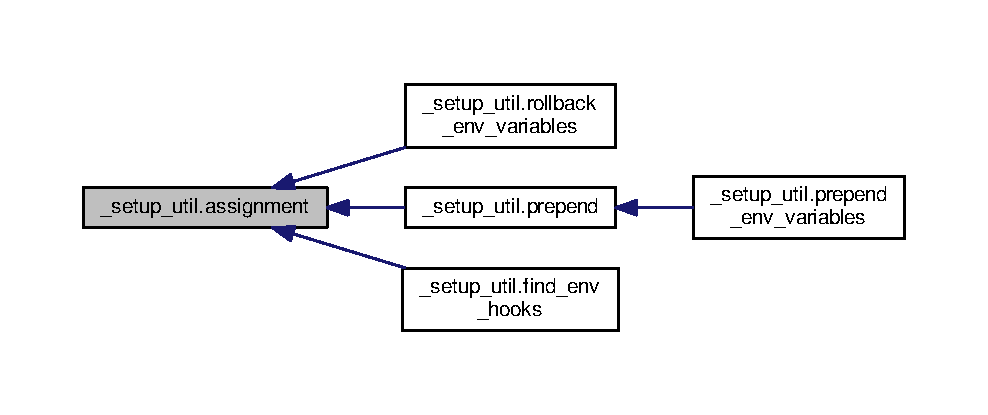
\includegraphics[width=350pt]{namespace__setup__util_ad56c24837fa4eddc63c03fbc7035628f_icgraph}
\end{center}
\end{figure}


\index{\+\_\+setup\+\_\+util@{\+\_\+setup\+\_\+util}!comment@{comment}}
\index{comment@{comment}!\+\_\+setup\+\_\+util@{\+\_\+setup\+\_\+util}}
\subsubsection[{\texorpdfstring{comment(msg)}{comment(msg)}}]{\setlength{\rightskip}{0pt plus 5cm}def \+\_\+setup\+\_\+util.\+comment (
\begin{DoxyParamCaption}
\item[{}]{msg}
\end{DoxyParamCaption}
)}\hypertarget{namespace__setup__util_abe8c95c4cfe8b1374dacd5f91d984353}{}\label{namespace__setup__util_abe8c95c4cfe8b1374dacd5f91d984353}


Definition at line 182 of file \+\_\+setup\+\_\+util.\+py.



Here is the caller graph for this function\+:
\nopagebreak
\begin{figure}[H]
\begin{center}
\leavevmode
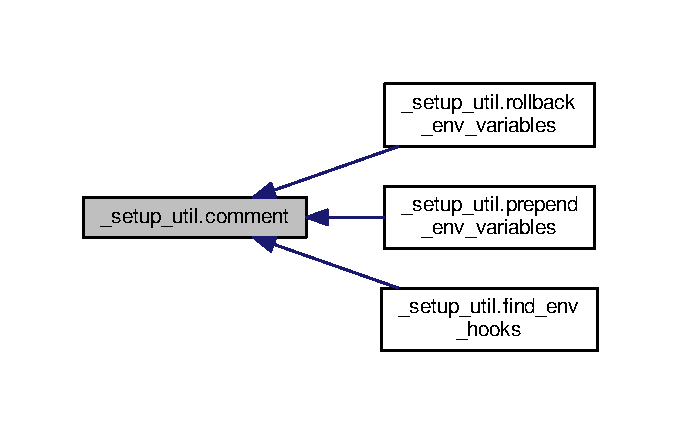
\includegraphics[width=327pt]{namespace__setup__util_abe8c95c4cfe8b1374dacd5f91d984353_icgraph}
\end{center}
\end{figure}


\index{\+\_\+setup\+\_\+util@{\+\_\+setup\+\_\+util}!find\+\_\+env\+\_\+hooks@{find\+\_\+env\+\_\+hooks}}
\index{find\+\_\+env\+\_\+hooks@{find\+\_\+env\+\_\+hooks}!\+\_\+setup\+\_\+util@{\+\_\+setup\+\_\+util}}
\subsubsection[{\texorpdfstring{find\+\_\+env\+\_\+hooks(environ, cmake\+\_\+prefix\+\_\+path)}{find_env_hooks(environ, cmake_prefix_path)}}]{\setlength{\rightskip}{0pt plus 5cm}def \+\_\+setup\+\_\+util.\+find\+\_\+env\+\_\+hooks (
\begin{DoxyParamCaption}
\item[{}]{environ, }
\item[{}]{cmake\+\_\+prefix\+\_\+path}
\end{DoxyParamCaption}
)}\hypertarget{namespace__setup__util_a73de35ca77f260af6691470342ab49ce}{}\label{namespace__setup__util_a73de35ca77f260af6691470342ab49ce}
\begin{DoxyVerb}Generate shell code with found environment hooks
for the all workspaces.
\end{DoxyVerb}
 

Definition at line 198 of file \+\_\+setup\+\_\+util.\+py.



Here is the call graph for this function\+:
\nopagebreak
\begin{figure}[H]
\begin{center}
\leavevmode
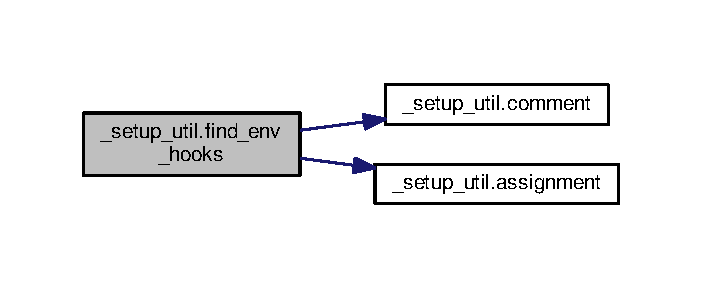
\includegraphics[width=337pt]{namespace__setup__util_a73de35ca77f260af6691470342ab49ce_cgraph}
\end{center}
\end{figure}


\index{\+\_\+setup\+\_\+util@{\+\_\+setup\+\_\+util}!prepend@{prepend}}
\index{prepend@{prepend}!\+\_\+setup\+\_\+util@{\+\_\+setup\+\_\+util}}
\subsubsection[{\texorpdfstring{prepend(environ, key, prefix)}{prepend(environ, key, prefix)}}]{\setlength{\rightskip}{0pt plus 5cm}def \+\_\+setup\+\_\+util.\+prepend (
\begin{DoxyParamCaption}
\item[{}]{environ, }
\item[{}]{key, }
\item[{}]{prefix}
\end{DoxyParamCaption}
)}\hypertarget{namespace__setup__util_ae78d86b2c4279f5b8b1acaa146c35802}{}\label{namespace__setup__util_ae78d86b2c4279f5b8b1acaa146c35802}


Definition at line 189 of file \+\_\+setup\+\_\+util.\+py.



Here is the call graph for this function\+:
\nopagebreak
\begin{figure}[H]
\begin{center}
\leavevmode
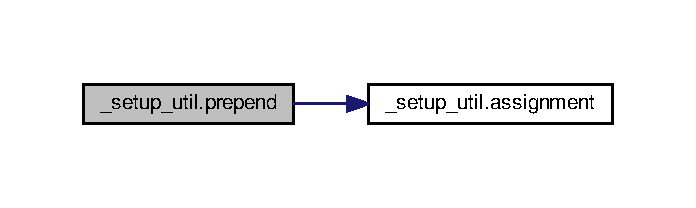
\includegraphics[width=334pt]{namespace__setup__util_ae78d86b2c4279f5b8b1acaa146c35802_cgraph}
\end{center}
\end{figure}




Here is the caller graph for this function\+:
\nopagebreak
\begin{figure}[H]
\begin{center}
\leavevmode
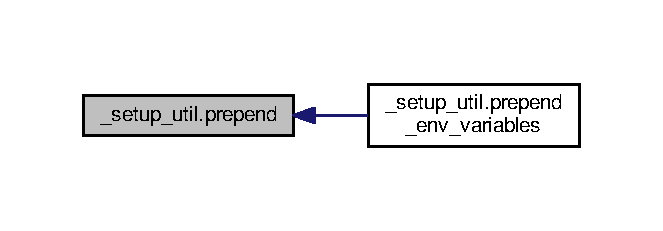
\includegraphics[width=318pt]{namespace__setup__util_ae78d86b2c4279f5b8b1acaa146c35802_icgraph}
\end{center}
\end{figure}


\index{\+\_\+setup\+\_\+util@{\+\_\+setup\+\_\+util}!prepend\+\_\+env\+\_\+variables@{prepend\+\_\+env\+\_\+variables}}
\index{prepend\+\_\+env\+\_\+variables@{prepend\+\_\+env\+\_\+variables}!\+\_\+setup\+\_\+util@{\+\_\+setup\+\_\+util}}
\subsubsection[{\texorpdfstring{prepend\+\_\+env\+\_\+variables(environ, env\+\_\+var\+\_\+subfolders, workspaces)}{prepend_env_variables(environ, env_var_subfolders, workspaces)}}]{\setlength{\rightskip}{0pt plus 5cm}def \+\_\+setup\+\_\+util.\+prepend\+\_\+env\+\_\+variables (
\begin{DoxyParamCaption}
\item[{}]{environ, }
\item[{}]{env\+\_\+var\+\_\+subfolders, }
\item[{}]{workspaces}
\end{DoxyParamCaption}
)}\hypertarget{namespace__setup__util_a832417d18b85bd1d276a87547e86f860}{}\label{namespace__setup__util_a832417d18b85bd1d276a87547e86f860}
\begin{DoxyVerb}Generate shell code to prepend environment variables
for the all workspaces.
\end{DoxyVerb}
 

Definition at line 129 of file \+\_\+setup\+\_\+util.\+py.



Here is the call graph for this function\+:
\nopagebreak
\begin{figure}[H]
\begin{center}
\leavevmode
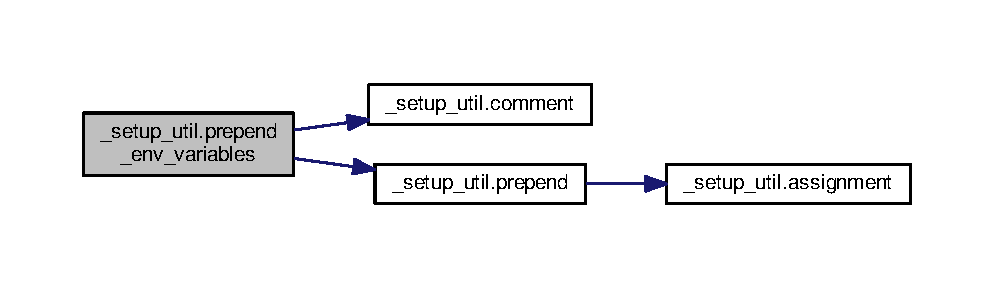
\includegraphics[width=350pt]{namespace__setup__util_a832417d18b85bd1d276a87547e86f860_cgraph}
\end{center}
\end{figure}


\index{\+\_\+setup\+\_\+util@{\+\_\+setup\+\_\+util}!rollback\+\_\+env\+\_\+variables@{rollback\+\_\+env\+\_\+variables}}
\index{rollback\+\_\+env\+\_\+variables@{rollback\+\_\+env\+\_\+variables}!\+\_\+setup\+\_\+util@{\+\_\+setup\+\_\+util}}
\subsubsection[{\texorpdfstring{rollback\+\_\+env\+\_\+variables(environ, env\+\_\+var\+\_\+subfolders)}{rollback_env_variables(environ, env_var_subfolders)}}]{\setlength{\rightskip}{0pt plus 5cm}def \+\_\+setup\+\_\+util.\+rollback\+\_\+env\+\_\+variables (
\begin{DoxyParamCaption}
\item[{}]{environ, }
\item[{}]{env\+\_\+var\+\_\+subfolders}
\end{DoxyParamCaption}
)}\hypertarget{namespace__setup__util_af3030db6102b5aa35cd354a2fb6cca03}{}\label{namespace__setup__util_af3030db6102b5aa35cd354a2fb6cca03}
\begin{DoxyVerb}Generate shell code to reset environment variables
by unrolling modifications based on all workspaces in CMAKE_PREFIX_PATH.
This does not cover modifications performed by environment hooks.
\end{DoxyVerb}
 

Definition at line 62 of file \+\_\+setup\+\_\+util.\+py.



Here is the call graph for this function\+:
\nopagebreak
\begin{figure}[H]
\begin{center}
\leavevmode
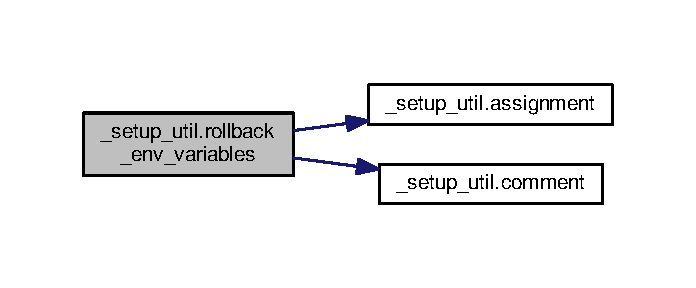
\includegraphics[width=334pt]{namespace__setup__util_af3030db6102b5aa35cd354a2fb6cca03_cgraph}
\end{center}
\end{figure}




\subsection{Variable Documentation}
\index{\+\_\+setup\+\_\+util@{\+\_\+setup\+\_\+util}!args@{args}}
\index{args@{args}!\+\_\+setup\+\_\+util@{\+\_\+setup\+\_\+util}}
\subsubsection[{\texorpdfstring{args}{args}}]{\setlength{\rightskip}{0pt plus 5cm}\+\_\+setup\+\_\+util.\+args = \+\_\+parse\+\_\+arguments()}\hypertarget{namespace__setup__util_a547963d07c6371df1c51b1384a2dec28}{}\label{namespace__setup__util_a547963d07c6371df1c51b1384a2dec28}


Definition at line 259 of file \+\_\+setup\+\_\+util.\+py.

\index{\+\_\+setup\+\_\+util@{\+\_\+setup\+\_\+util}!base\+\_\+path@{base\+\_\+path}}
\index{base\+\_\+path@{base\+\_\+path}!\+\_\+setup\+\_\+util@{\+\_\+setup\+\_\+util}}
\subsubsection[{\texorpdfstring{base\+\_\+path}{base_path}}]{\setlength{\rightskip}{0pt plus 5cm}\+\_\+setup\+\_\+util.\+base\+\_\+path = os.\+path.\+dirname(\+\_\+\+\_\+file\+\_\+\+\_\+)}\hypertarget{namespace__setup__util_a83d25140acd7788bbcb95843fe38e639}{}\label{namespace__setup__util_a83d25140acd7788bbcb95843fe38e639}


Definition at line 267 of file \+\_\+setup\+\_\+util.\+py.

\index{\+\_\+setup\+\_\+util@{\+\_\+setup\+\_\+util}!C\+A\+T\+K\+I\+N\+\_\+\+M\+A\+R\+K\+E\+R\+\_\+\+F\+I\+LE@{C\+A\+T\+K\+I\+N\+\_\+\+M\+A\+R\+K\+E\+R\+\_\+\+F\+I\+LE}}
\index{C\+A\+T\+K\+I\+N\+\_\+\+M\+A\+R\+K\+E\+R\+\_\+\+F\+I\+LE@{C\+A\+T\+K\+I\+N\+\_\+\+M\+A\+R\+K\+E\+R\+\_\+\+F\+I\+LE}!\+\_\+setup\+\_\+util@{\+\_\+setup\+\_\+util}}
\subsubsection[{\texorpdfstring{C\+A\+T\+K\+I\+N\+\_\+\+M\+A\+R\+K\+E\+R\+\_\+\+F\+I\+LE}{CATKIN_MARKER_FILE}}]{\setlength{\rightskip}{0pt plus 5cm}string \+\_\+setup\+\_\+util.\+C\+A\+T\+K\+I\+N\+\_\+\+M\+A\+R\+K\+E\+R\+\_\+\+F\+I\+LE = \textquotesingle{}.catkin\textquotesingle{}}\hypertarget{namespace__setup__util_a3fa0ca5a460a71a43cbc3d4954ab1f10}{}\label{namespace__setup__util_a3fa0ca5a460a71a43cbc3d4954ab1f10}


Definition at line 46 of file \+\_\+setup\+\_\+util.\+py.

\index{\+\_\+setup\+\_\+util@{\+\_\+setup\+\_\+util}!C\+M\+A\+K\+E\+\_\+\+P\+R\+E\+F\+I\+X\+\_\+\+P\+A\+TH@{C\+M\+A\+K\+E\+\_\+\+P\+R\+E\+F\+I\+X\+\_\+\+P\+A\+TH}}
\index{C\+M\+A\+K\+E\+\_\+\+P\+R\+E\+F\+I\+X\+\_\+\+P\+A\+TH@{C\+M\+A\+K\+E\+\_\+\+P\+R\+E\+F\+I\+X\+\_\+\+P\+A\+TH}!\+\_\+setup\+\_\+util@{\+\_\+setup\+\_\+util}}
\subsubsection[{\texorpdfstring{C\+M\+A\+K\+E\+\_\+\+P\+R\+E\+F\+I\+X\+\_\+\+P\+A\+TH}{CMAKE_PREFIX_PATH}}]{\setlength{\rightskip}{0pt plus 5cm}string \+\_\+setup\+\_\+util.\+C\+M\+A\+K\+E\+\_\+\+P\+R\+E\+F\+I\+X\+\_\+\+P\+A\+TH = \textquotesingle{}/home/jbs/catkin\+\_\+ws/devel;/opt/ros/kinetic\textquotesingle{}}\hypertarget{namespace__setup__util_a57afd3d2c076955fb715f3e72ef098eb}{}\label{namespace__setup__util_a57afd3d2c076955fb715f3e72ef098eb}


Definition at line 265 of file \+\_\+setup\+\_\+util.\+py.

\index{\+\_\+setup\+\_\+util@{\+\_\+setup\+\_\+util}!e@{e}}
\index{e@{e}!\+\_\+setup\+\_\+util@{\+\_\+setup\+\_\+util}}
\subsubsection[{\texorpdfstring{e}{e}}]{\setlength{\rightskip}{0pt plus 5cm}\+\_\+setup\+\_\+util.\+e}\hypertarget{namespace__setup__util_acdce690b925de33d6249bbbfa1109d61}{}\label{namespace__setup__util_acdce690b925de33d6249bbbfa1109d61}


Definition at line 261 of file \+\_\+setup\+\_\+util.\+py.

\index{\+\_\+setup\+\_\+util@{\+\_\+setup\+\_\+util}!E\+N\+V\+\_\+\+V\+A\+R\+\_\+\+S\+U\+B\+F\+O\+L\+D\+E\+RS@{E\+N\+V\+\_\+\+V\+A\+R\+\_\+\+S\+U\+B\+F\+O\+L\+D\+E\+RS}}
\index{E\+N\+V\+\_\+\+V\+A\+R\+\_\+\+S\+U\+B\+F\+O\+L\+D\+E\+RS@{E\+N\+V\+\_\+\+V\+A\+R\+\_\+\+S\+U\+B\+F\+O\+L\+D\+E\+RS}!\+\_\+setup\+\_\+util@{\+\_\+setup\+\_\+util}}
\subsubsection[{\texorpdfstring{E\+N\+V\+\_\+\+V\+A\+R\+\_\+\+S\+U\+B\+F\+O\+L\+D\+E\+RS}{ENV_VAR_SUBFOLDERS}}]{\setlength{\rightskip}{0pt plus 5cm}dictionary \+\_\+setup\+\_\+util.\+E\+N\+V\+\_\+\+V\+A\+R\+\_\+\+S\+U\+B\+F\+O\+L\+D\+E\+RS}\hypertarget{namespace__setup__util_aa31804f1be8660156ce9394b33c68dc4}{}\label{namespace__setup__util_aa31804f1be8660156ce9394b33c68dc4}
{\bfseries Initial value\+:}
\begin{DoxyCode}
1 = \{
2     \textcolor{stringliteral}{'CMAKE\_PREFIX\_PATH'}: \textcolor{stringliteral}{''},
3     \textcolor{stringliteral}{'LD\_LIBRARY\_PATH'} \textcolor{keywordflow}{if} \textcolor{keywordflow}{not} IS\_DARWIN \textcolor{keywordflow}{else} \textcolor{stringliteral}{'DYLD\_LIBRARY\_PATH'}: [\textcolor{stringliteral}{'lib'}, os.path.join(\textcolor{stringliteral}{'lib'}, \textcolor{stringliteral}{'
      x86\_64-linux-gnu'})],
4     \textcolor{stringliteral}{'PATH'}: \textcolor{stringliteral}{'bin'},
5     \textcolor{stringliteral}{'PKG\_CONFIG\_PATH'}: [os.path.join(\textcolor{stringliteral}{'lib'}, \textcolor{stringliteral}{'pkgconfig'}), os.path.join(\textcolor{stringliteral}{'lib'}, \textcolor{stringliteral}{'x86\_64-linux-gnu'}, \textcolor{stringliteral}{'
      pkgconfig'})],
6     \textcolor{stringliteral}{'PYTHONPATH'}: \textcolor{stringliteral}{'lib/python2.7/dist-packages'},
7 \}
\end{DoxyCode}


Definition at line 53 of file \+\_\+setup\+\_\+util.\+py.

\index{\+\_\+setup\+\_\+util@{\+\_\+setup\+\_\+util}!environ@{environ}}
\index{environ@{environ}!\+\_\+setup\+\_\+util@{\+\_\+setup\+\_\+util}}
\subsubsection[{\texorpdfstring{environ}{environ}}]{\setlength{\rightskip}{0pt plus 5cm}\+\_\+setup\+\_\+util.\+environ = dict(os.\+environ)}\hypertarget{namespace__setup__util_a9a935bdd9ee1aa0327161025bb18c136}{}\label{namespace__setup__util_a9a935bdd9ee1aa0327161025bb18c136}


Definition at line 272 of file \+\_\+setup\+\_\+util.\+py.

\index{\+\_\+setup\+\_\+util@{\+\_\+setup\+\_\+util}!file@{file}}
\index{file@{file}!\+\_\+setup\+\_\+util@{\+\_\+setup\+\_\+util}}
\subsubsection[{\texorpdfstring{file}{file}}]{\setlength{\rightskip}{0pt plus 5cm}\+\_\+setup\+\_\+util.\+file}\hypertarget{namespace__setup__util_aea63a1b32cc79bc3d872ab7cb30dd07e}{}\label{namespace__setup__util_aea63a1b32cc79bc3d872ab7cb30dd07e}


Definition at line 261 of file \+\_\+setup\+\_\+util.\+py.

\index{\+\_\+setup\+\_\+util@{\+\_\+setup\+\_\+util}!I\+S\+\_\+\+D\+A\+R\+W\+IN@{I\+S\+\_\+\+D\+A\+R\+W\+IN}}
\index{I\+S\+\_\+\+D\+A\+R\+W\+IN@{I\+S\+\_\+\+D\+A\+R\+W\+IN}!\+\_\+setup\+\_\+util@{\+\_\+setup\+\_\+util}}
\subsubsection[{\texorpdfstring{I\+S\+\_\+\+D\+A\+R\+W\+IN}{IS_DARWIN}}]{\setlength{\rightskip}{0pt plus 5cm}tuple \+\_\+setup\+\_\+util.\+I\+S\+\_\+\+D\+A\+R\+W\+IN = ({\bf system} == \textquotesingle{}Darwin\textquotesingle{})}\hypertarget{namespace__setup__util_aecbb100ce6f94bb3c7e16d58fde05f96}{}\label{namespace__setup__util_aecbb100ce6f94bb3c7e16d58fde05f96}


Definition at line 49 of file \+\_\+setup\+\_\+util.\+py.

\index{\+\_\+setup\+\_\+util@{\+\_\+setup\+\_\+util}!I\+S\+\_\+\+W\+I\+N\+D\+O\+WS@{I\+S\+\_\+\+W\+I\+N\+D\+O\+WS}}
\index{I\+S\+\_\+\+W\+I\+N\+D\+O\+WS@{I\+S\+\_\+\+W\+I\+N\+D\+O\+WS}!\+\_\+setup\+\_\+util@{\+\_\+setup\+\_\+util}}
\subsubsection[{\texorpdfstring{I\+S\+\_\+\+W\+I\+N\+D\+O\+WS}{IS_WINDOWS}}]{\setlength{\rightskip}{0pt plus 5cm}tuple \+\_\+setup\+\_\+util.\+I\+S\+\_\+\+W\+I\+N\+D\+O\+WS = ({\bf system} == \textquotesingle{}Windows\textquotesingle{})}\hypertarget{namespace__setup__util_a6fe69c2dbd92959b6651a28cbb846e6e}{}\label{namespace__setup__util_a6fe69c2dbd92959b6651a28cbb846e6e}


Definition at line 50 of file \+\_\+setup\+\_\+util.\+py.

\index{\+\_\+setup\+\_\+util@{\+\_\+setup\+\_\+util}!lines@{lines}}
\index{lines@{lines}!\+\_\+setup\+\_\+util@{\+\_\+setup\+\_\+util}}
\subsubsection[{\texorpdfstring{lines}{lines}}]{\setlength{\rightskip}{0pt plus 5cm}list \+\_\+setup\+\_\+util.\+lines = \mbox{[}$\,$\mbox{]}}\hypertarget{namespace__setup__util_a8618d8be5f729d4c9696daa5e083a001}{}\label{namespace__setup__util_a8618d8be5f729d4c9696daa5e083a001}


Definition at line 273 of file \+\_\+setup\+\_\+util.\+py.

\index{\+\_\+setup\+\_\+util@{\+\_\+setup\+\_\+util}!system@{system}}
\index{system@{system}!\+\_\+setup\+\_\+util@{\+\_\+setup\+\_\+util}}
\subsubsection[{\texorpdfstring{system}{system}}]{\setlength{\rightskip}{0pt plus 5cm}\+\_\+setup\+\_\+util.\+system = platform.\+system()}\hypertarget{namespace__setup__util_ae9fca6a80a6923f4580be72f68fee325}{}\label{namespace__setup__util_ae9fca6a80a6923f4580be72f68fee325}


Definition at line 48 of file \+\_\+setup\+\_\+util.\+py.


\hypertarget{namespace_c_h_o_m_p}{}\section{C\+H\+O\+MP Namespace Reference}
\label{namespace_c_h_o_m_p}\index{C\+H\+O\+MP@{C\+H\+O\+MP}}


This script solves the \hyperlink{namespace_c_h_o_m_p}{C\+H\+O\+MP} programming \+: 1/2 x\textquotesingle{}Ax + bx + f(x) This requires evaluation function for f(x) and grad\+\_\+f(x) as a function pointer and other parameter.  


\subsection*{Classes}
\begin{DoxyCompactItemize}
\item 
class \hyperlink{class_c_h_o_m_p_1_1_chomp_forecaster}{Chomp\+Forecaster}
\item 
struct \hyperlink{struct_c_h_o_m_p_1_1_cost_param}{Cost\+Param}
\item 
struct \hyperlink{struct_c_h_o_m_p_1_1_optim_grad}{Optim\+Grad}
\begin{DoxyCompactList}\small\item\em gradient containing prior and nonlinear together \end{DoxyCompactList}\item 
struct \hyperlink{struct_c_h_o_m_p_1_1_optim_info}{Optim\+Info}
\item 
struct \hyperlink{struct_c_h_o_m_p_1_1_optim_param}{Optim\+Param}
\item 
struct \hyperlink{struct_c_h_o_m_p_1_1_optim_result}{Optim\+Result}
\item 
struct \hyperlink{struct_c_h_o_m_p_1_1_prediction_trajectory}{Prediction\+Trajectory}
\item 
struct \hyperlink{struct_c_h_o_m_p_1_1_predict_param}{Predict\+Param}
\item 
class \hyperlink{class_c_h_o_m_p_1_1_solver}{Solver}
\item 
class \hyperlink{class_c_h_o_m_p_1_1_wrapper}{Wrapper}
\end{DoxyCompactItemize}


\subsection{Detailed Description}
This script solves the \hyperlink{namespace_c_h_o_m_p}{C\+H\+O\+MP} programming \+: 1/2 x\textquotesingle{}Ax + bx + f(x) This requires evaluation function for f(x) and grad\+\_\+f(x) as a function pointer and other parameter. 
\hypertarget{namespacegenerate__cached__setup}{}\section{generate\+\_\+cached\+\_\+setup Namespace Reference}
\label{namespacegenerate__cached__setup}\index{generate\+\_\+cached\+\_\+setup@{generate\+\_\+cached\+\_\+setup}}
\subsection*{Variables}
\begin{DoxyCompactItemize}
\item 
\hyperlink{namespacegenerate__cached__setup_a72579fd01529a79bab20d99291889d3f}{python\+\_\+path} = os.\+path.\+join(workspace, \textquotesingle{}lib/python2.\+7/dist-\/packages\textquotesingle{})
\item 
\hyperlink{namespacegenerate__cached__setup_a52601295006f2366a311c4453d8f2f2e}{code} = generate\+\_\+environment\+\_\+script(\textquotesingle{}/home/jbs/catkin\+\_\+ws/src/chomp\+\_\+predict/build/devel/env.\+sh\textquotesingle{})
\item 
string \hyperlink{namespacegenerate__cached__setup_a0265aee5075ee1eb701ff69c98ad6793}{output\+\_\+filename} = \textquotesingle{}/home/jbs/catkin\+\_\+ws/src/chomp\+\_\+predict/build/catkin\+\_\+generated/setup\+\_\+cached.\+sh\textquotesingle{}
\item 
\hyperlink{namespacegenerate__cached__setup_a10081e5abedae9bd46dd91202096e789}{mode} = os.\+stat(\hyperlink{namespacegenerate__cached__setup_a0265aee5075ee1eb701ff69c98ad6793}{output\+\_\+filename}).st\+\_\+mode
\end{DoxyCompactItemize}


\subsection{Variable Documentation}
\index{generate\+\_\+cached\+\_\+setup@{generate\+\_\+cached\+\_\+setup}!code@{code}}
\index{code@{code}!generate\+\_\+cached\+\_\+setup@{generate\+\_\+cached\+\_\+setup}}
\subsubsection[{\texorpdfstring{code}{code}}]{\setlength{\rightskip}{0pt plus 5cm}generate\+\_\+cached\+\_\+setup.\+code = generate\+\_\+environment\+\_\+script(\textquotesingle{}/home/jbs/catkin\+\_\+ws/src/chomp\+\_\+predict/build/devel/env.\+sh\textquotesingle{})}\hypertarget{namespacegenerate__cached__setup_a52601295006f2366a311c4453d8f2f2e}{}\label{namespacegenerate__cached__setup_a52601295006f2366a311c4453d8f2f2e}


Definition at line 22 of file generate\+\_\+cached\+\_\+setup.\+py.

\index{generate\+\_\+cached\+\_\+setup@{generate\+\_\+cached\+\_\+setup}!mode@{mode}}
\index{mode@{mode}!generate\+\_\+cached\+\_\+setup@{generate\+\_\+cached\+\_\+setup}}
\subsubsection[{\texorpdfstring{mode}{mode}}]{\setlength{\rightskip}{0pt plus 5cm}generate\+\_\+cached\+\_\+setup.\+mode = os.\+stat({\bf output\+\_\+filename}).st\+\_\+mode}\hypertarget{namespacegenerate__cached__setup_a10081e5abedae9bd46dd91202096e789}{}\label{namespacegenerate__cached__setup_a10081e5abedae9bd46dd91202096e789}


Definition at line 29 of file generate\+\_\+cached\+\_\+setup.\+py.

\index{generate\+\_\+cached\+\_\+setup@{generate\+\_\+cached\+\_\+setup}!output\+\_\+filename@{output\+\_\+filename}}
\index{output\+\_\+filename@{output\+\_\+filename}!generate\+\_\+cached\+\_\+setup@{generate\+\_\+cached\+\_\+setup}}
\subsubsection[{\texorpdfstring{output\+\_\+filename}{output_filename}}]{\setlength{\rightskip}{0pt plus 5cm}string generate\+\_\+cached\+\_\+setup.\+output\+\_\+filename = \textquotesingle{}/home/jbs/catkin\+\_\+ws/src/chomp\+\_\+predict/build/catkin\+\_\+generated/setup\+\_\+cached.\+sh\textquotesingle{}}\hypertarget{namespacegenerate__cached__setup_a0265aee5075ee1eb701ff69c98ad6793}{}\label{namespacegenerate__cached__setup_a0265aee5075ee1eb701ff69c98ad6793}


Definition at line 24 of file generate\+\_\+cached\+\_\+setup.\+py.

\index{generate\+\_\+cached\+\_\+setup@{generate\+\_\+cached\+\_\+setup}!python\+\_\+path@{python\+\_\+path}}
\index{python\+\_\+path@{python\+\_\+path}!generate\+\_\+cached\+\_\+setup@{generate\+\_\+cached\+\_\+setup}}
\subsubsection[{\texorpdfstring{python\+\_\+path}{python_path}}]{\setlength{\rightskip}{0pt plus 5cm}generate\+\_\+cached\+\_\+setup.\+python\+\_\+path = os.\+path.\+join(workspace, \textquotesingle{}lib/python2.\+7/dist-\/packages\textquotesingle{})}\hypertarget{namespacegenerate__cached__setup_a72579fd01529a79bab20d99291889d3f}{}\label{namespacegenerate__cached__setup_a72579fd01529a79bab20d99291889d3f}


Definition at line 16 of file generate\+\_\+cached\+\_\+setup.\+py.


\hypertarget{namespacepkg}{}\section{pkg Namespace Reference}
\label{namespacepkg}\index{pkg@{pkg}}
\subsection*{Variables}
\begin{DoxyCompactItemize}
\item 
string \hyperlink{namespacepkg_ae26c7a5a06b7d738f4d210ca449e6bee}{C\+A\+T\+K\+I\+N\+\_\+\+P\+A\+C\+K\+A\+G\+E\+\_\+\+P\+R\+E\+F\+IX} = \char`\"{}\char`\"{}
\item 
string \hyperlink{namespacepkg_a2760bf8266ff58da440f65ee91b203ab}{P\+R\+O\+J\+E\+C\+T\+\_\+\+P\+K\+G\+\_\+\+C\+O\+N\+F\+I\+G\+\_\+\+I\+N\+C\+L\+U\+D\+E\+\_\+\+D\+I\+RS} = \char`\"{}/home/jbs/catkin\+\_\+ws/src/chomp\+\_\+predict/include\char`\"{}
\item 
string \hyperlink{namespacepkg_a17c18447fad253ee1c0d76deec88028c}{P\+R\+O\+J\+E\+C\+T\+\_\+\+C\+A\+T\+K\+I\+N\+\_\+\+D\+E\+P\+E\+N\+DS} = \char`\"{}\char`\"{}
\item 
string \hyperlink{namespacepkg_a433e30cecb4a0123a7c4b384d168e336}{P\+K\+G\+\_\+\+C\+O\+N\+F\+I\+G\+\_\+\+L\+I\+B\+R\+A\+R\+I\+E\+S\+\_\+\+W\+I\+T\+H\+\_\+\+P\+R\+E\+F\+IX} = \char`\"{}-\/lchomp\+\_\+predict\char`\"{}
\item 
string \hyperlink{namespacepkg_a7dfbe99257c26f5e4a3a5483995d9ddc}{P\+R\+O\+J\+E\+C\+T\+\_\+\+N\+A\+ME} = \char`\"{}chomp\+\_\+predict\char`\"{}
\item 
string \hyperlink{namespacepkg_a3f0f1b4bc03c596525e025539ca4332f}{P\+R\+O\+J\+E\+C\+T\+\_\+\+S\+P\+A\+C\+E\+\_\+\+D\+IR} = \char`\"{}/home/jbs/catkin\+\_\+ws/src/chomp\+\_\+predict/build/devel\char`\"{}
\item 
string \hyperlink{namespacepkg_ab1037914b9286bb61855131c06149648}{P\+R\+O\+J\+E\+C\+T\+\_\+\+V\+E\+R\+S\+I\+ON} = \char`\"{}0.\+0.\+0\char`\"{}
\end{DoxyCompactItemize}


\subsection{Variable Documentation}
\index{pkg@{pkg}!C\+A\+T\+K\+I\+N\+\_\+\+P\+A\+C\+K\+A\+G\+E\+\_\+\+P\+R\+E\+F\+IX@{C\+A\+T\+K\+I\+N\+\_\+\+P\+A\+C\+K\+A\+G\+E\+\_\+\+P\+R\+E\+F\+IX}}
\index{C\+A\+T\+K\+I\+N\+\_\+\+P\+A\+C\+K\+A\+G\+E\+\_\+\+P\+R\+E\+F\+IX@{C\+A\+T\+K\+I\+N\+\_\+\+P\+A\+C\+K\+A\+G\+E\+\_\+\+P\+R\+E\+F\+IX}!pkg@{pkg}}
\subsubsection[{\texorpdfstring{C\+A\+T\+K\+I\+N\+\_\+\+P\+A\+C\+K\+A\+G\+E\+\_\+\+P\+R\+E\+F\+IX}{CATKIN_PACKAGE_PREFIX}}]{\setlength{\rightskip}{0pt plus 5cm}string pkg.\+C\+A\+T\+K\+I\+N\+\_\+\+P\+A\+C\+K\+A\+G\+E\+\_\+\+P\+R\+E\+F\+IX = \char`\"{}\char`\"{}}\hypertarget{namespacepkg_ae26c7a5a06b7d738f4d210ca449e6bee}{}\label{namespacepkg_ae26c7a5a06b7d738f4d210ca449e6bee}


Definition at line 2 of file pkg.\+develspace.\+context.\+pc.\+py.

\index{pkg@{pkg}!P\+K\+G\+\_\+\+C\+O\+N\+F\+I\+G\+\_\+\+L\+I\+B\+R\+A\+R\+I\+E\+S\+\_\+\+W\+I\+T\+H\+\_\+\+P\+R\+E\+F\+IX@{P\+K\+G\+\_\+\+C\+O\+N\+F\+I\+G\+\_\+\+L\+I\+B\+R\+A\+R\+I\+E\+S\+\_\+\+W\+I\+T\+H\+\_\+\+P\+R\+E\+F\+IX}}
\index{P\+K\+G\+\_\+\+C\+O\+N\+F\+I\+G\+\_\+\+L\+I\+B\+R\+A\+R\+I\+E\+S\+\_\+\+W\+I\+T\+H\+\_\+\+P\+R\+E\+F\+IX@{P\+K\+G\+\_\+\+C\+O\+N\+F\+I\+G\+\_\+\+L\+I\+B\+R\+A\+R\+I\+E\+S\+\_\+\+W\+I\+T\+H\+\_\+\+P\+R\+E\+F\+IX}!pkg@{pkg}}
\subsubsection[{\texorpdfstring{P\+K\+G\+\_\+\+C\+O\+N\+F\+I\+G\+\_\+\+L\+I\+B\+R\+A\+R\+I\+E\+S\+\_\+\+W\+I\+T\+H\+\_\+\+P\+R\+E\+F\+IX}{PKG_CONFIG_LIBRARIES_WITH_PREFIX}}]{\setlength{\rightskip}{0pt plus 5cm}string pkg.\+P\+K\+G\+\_\+\+C\+O\+N\+F\+I\+G\+\_\+\+L\+I\+B\+R\+A\+R\+I\+E\+S\+\_\+\+W\+I\+T\+H\+\_\+\+P\+R\+E\+F\+IX = \char`\"{}-\/lchomp\+\_\+predict\char`\"{}}\hypertarget{namespacepkg_a433e30cecb4a0123a7c4b384d168e336}{}\label{namespacepkg_a433e30cecb4a0123a7c4b384d168e336}


Definition at line 5 of file pkg.\+develspace.\+context.\+pc.\+py.

\index{pkg@{pkg}!P\+R\+O\+J\+E\+C\+T\+\_\+\+C\+A\+T\+K\+I\+N\+\_\+\+D\+E\+P\+E\+N\+DS@{P\+R\+O\+J\+E\+C\+T\+\_\+\+C\+A\+T\+K\+I\+N\+\_\+\+D\+E\+P\+E\+N\+DS}}
\index{P\+R\+O\+J\+E\+C\+T\+\_\+\+C\+A\+T\+K\+I\+N\+\_\+\+D\+E\+P\+E\+N\+DS@{P\+R\+O\+J\+E\+C\+T\+\_\+\+C\+A\+T\+K\+I\+N\+\_\+\+D\+E\+P\+E\+N\+DS}!pkg@{pkg}}
\subsubsection[{\texorpdfstring{P\+R\+O\+J\+E\+C\+T\+\_\+\+C\+A\+T\+K\+I\+N\+\_\+\+D\+E\+P\+E\+N\+DS}{PROJECT_CATKIN_DEPENDS}}]{\setlength{\rightskip}{0pt plus 5cm}string pkg.\+P\+R\+O\+J\+E\+C\+T\+\_\+\+C\+A\+T\+K\+I\+N\+\_\+\+D\+E\+P\+E\+N\+DS = \char`\"{}\char`\"{}}\hypertarget{namespacepkg_a17c18447fad253ee1c0d76deec88028c}{}\label{namespacepkg_a17c18447fad253ee1c0d76deec88028c}


Definition at line 4 of file pkg.\+develspace.\+context.\+pc.\+py.

\index{pkg@{pkg}!P\+R\+O\+J\+E\+C\+T\+\_\+\+N\+A\+ME@{P\+R\+O\+J\+E\+C\+T\+\_\+\+N\+A\+ME}}
\index{P\+R\+O\+J\+E\+C\+T\+\_\+\+N\+A\+ME@{P\+R\+O\+J\+E\+C\+T\+\_\+\+N\+A\+ME}!pkg@{pkg}}
\subsubsection[{\texorpdfstring{P\+R\+O\+J\+E\+C\+T\+\_\+\+N\+A\+ME}{PROJECT_NAME}}]{\setlength{\rightskip}{0pt plus 5cm}string pkg.\+P\+R\+O\+J\+E\+C\+T\+\_\+\+N\+A\+ME = \char`\"{}chomp\+\_\+predict\char`\"{}}\hypertarget{namespacepkg_a7dfbe99257c26f5e4a3a5483995d9ddc}{}\label{namespacepkg_a7dfbe99257c26f5e4a3a5483995d9ddc}


Definition at line 6 of file pkg.\+develspace.\+context.\+pc.\+py.

\index{pkg@{pkg}!P\+R\+O\+J\+E\+C\+T\+\_\+\+P\+K\+G\+\_\+\+C\+O\+N\+F\+I\+G\+\_\+\+I\+N\+C\+L\+U\+D\+E\+\_\+\+D\+I\+RS@{P\+R\+O\+J\+E\+C\+T\+\_\+\+P\+K\+G\+\_\+\+C\+O\+N\+F\+I\+G\+\_\+\+I\+N\+C\+L\+U\+D\+E\+\_\+\+D\+I\+RS}}
\index{P\+R\+O\+J\+E\+C\+T\+\_\+\+P\+K\+G\+\_\+\+C\+O\+N\+F\+I\+G\+\_\+\+I\+N\+C\+L\+U\+D\+E\+\_\+\+D\+I\+RS@{P\+R\+O\+J\+E\+C\+T\+\_\+\+P\+K\+G\+\_\+\+C\+O\+N\+F\+I\+G\+\_\+\+I\+N\+C\+L\+U\+D\+E\+\_\+\+D\+I\+RS}!pkg@{pkg}}
\subsubsection[{\texorpdfstring{P\+R\+O\+J\+E\+C\+T\+\_\+\+P\+K\+G\+\_\+\+C\+O\+N\+F\+I\+G\+\_\+\+I\+N\+C\+L\+U\+D\+E\+\_\+\+D\+I\+RS}{PROJECT_PKG_CONFIG_INCLUDE_DIRS}}]{\setlength{\rightskip}{0pt plus 5cm}string pkg.\+P\+R\+O\+J\+E\+C\+T\+\_\+\+P\+K\+G\+\_\+\+C\+O\+N\+F\+I\+G\+\_\+\+I\+N\+C\+L\+U\+D\+E\+\_\+\+D\+I\+RS = \char`\"{}/home/jbs/catkin\+\_\+ws/src/chomp\+\_\+predict/include\char`\"{}}\hypertarget{namespacepkg_a2760bf8266ff58da440f65ee91b203ab}{}\label{namespacepkg_a2760bf8266ff58da440f65ee91b203ab}


Definition at line 3 of file pkg.\+develspace.\+context.\+pc.\+py.

\index{pkg@{pkg}!P\+R\+O\+J\+E\+C\+T\+\_\+\+S\+P\+A\+C\+E\+\_\+\+D\+IR@{P\+R\+O\+J\+E\+C\+T\+\_\+\+S\+P\+A\+C\+E\+\_\+\+D\+IR}}
\index{P\+R\+O\+J\+E\+C\+T\+\_\+\+S\+P\+A\+C\+E\+\_\+\+D\+IR@{P\+R\+O\+J\+E\+C\+T\+\_\+\+S\+P\+A\+C\+E\+\_\+\+D\+IR}!pkg@{pkg}}
\subsubsection[{\texorpdfstring{P\+R\+O\+J\+E\+C\+T\+\_\+\+S\+P\+A\+C\+E\+\_\+\+D\+IR}{PROJECT_SPACE_DIR}}]{\setlength{\rightskip}{0pt plus 5cm}string pkg.\+P\+R\+O\+J\+E\+C\+T\+\_\+\+S\+P\+A\+C\+E\+\_\+\+D\+IR = \char`\"{}/home/jbs/catkin\+\_\+ws/src/chomp\+\_\+predict/build/devel\char`\"{}}\hypertarget{namespacepkg_a3f0f1b4bc03c596525e025539ca4332f}{}\label{namespacepkg_a3f0f1b4bc03c596525e025539ca4332f}


Definition at line 7 of file pkg.\+develspace.\+context.\+pc.\+py.

\index{pkg@{pkg}!P\+R\+O\+J\+E\+C\+T\+\_\+\+V\+E\+R\+S\+I\+ON@{P\+R\+O\+J\+E\+C\+T\+\_\+\+V\+E\+R\+S\+I\+ON}}
\index{P\+R\+O\+J\+E\+C\+T\+\_\+\+V\+E\+R\+S\+I\+ON@{P\+R\+O\+J\+E\+C\+T\+\_\+\+V\+E\+R\+S\+I\+ON}!pkg@{pkg}}
\subsubsection[{\texorpdfstring{P\+R\+O\+J\+E\+C\+T\+\_\+\+V\+E\+R\+S\+I\+ON}{PROJECT_VERSION}}]{\setlength{\rightskip}{0pt plus 5cm}string pkg.\+P\+R\+O\+J\+E\+C\+T\+\_\+\+V\+E\+R\+S\+I\+ON = \char`\"{}0.\+0.\+0\char`\"{}}\hypertarget{namespacepkg_ab1037914b9286bb61855131c06149648}{}\label{namespacepkg_ab1037914b9286bb61855131c06149648}


Definition at line 8 of file pkg.\+develspace.\+context.\+pc.\+py.


\chapter{Class Documentation}
\hypertarget{class_c_h_o_m_p_1_1_chomp_forecaster}{}\section{C\+H\+O\+MP\+:\+:Chomp\+Forecaster Class Reference}
\label{class_c_h_o_m_p_1_1_chomp_forecaster}\index{C\+H\+O\+M\+P\+::\+Chomp\+Forecaster@{C\+H\+O\+M\+P\+::\+Chomp\+Forecaster}}


{\ttfamily \#include $<$chomp\+\_\+predict.\+h$>$}

\subsection*{Public Member Functions}
\begin{DoxyCompactItemize}
\item 
\hyperlink{class_c_h_o_m_p_1_1_chomp_forecaster_a58176b34170de8485029f182e05f12c5}{Chomp\+Forecaster} ()
\item 
void \hyperlink{class_c_h_o_m_p_1_1_chomp_forecaster_ac05e634464c8859c8cc3e8bdb1a40ded}{callback\+\_\+target\+\_\+state} (geometry\+\_\+msgs\+::\+Pose\+Stamped\+Const\+Ptr pose\+\_\+stamped\+\_\+ptr)
\item 
void \hyperlink{class_c_h_o_m_p_1_1_chomp_forecaster_a02a3930b78aaf72a9058cb3ce6ae8143}{predict\+\_\+with\+\_\+obsrv\+\_\+queue} ()
\item 
geometry\+\_\+msgs\+::\+Point \hyperlink{class_c_h_o_m_p_1_1_chomp_forecaster_a8b3e5ea0d8a5092b371a23efcddd5c73}{eval\+\_\+prediction} (ros\+::\+Time eval\+\_\+time)
\begin{DoxyCompactList}\small\item\em Once prediction model is acquired, then we can evaluate the prediction in time. \end{DoxyCompactList}\item 
void \hyperlink{class_c_h_o_m_p_1_1_chomp_forecaster_a56e9984f3c85563170c58708aaa97056}{publish\+\_\+routine} ()
\begin{DoxyCompactList}\small\item\em publish routine in while loop \end{DoxyCompactList}\item 
void \hyperlink{class_c_h_o_m_p_1_1_chomp_forecaster_af225bf2af3fede364b922e27be410f0b}{run} ()
\begin{DoxyCompactList}\small\item\em code to be run in the main loop \end{DoxyCompactList}\end{DoxyCompactItemize}
\subsection*{Public Attributes}
\begin{DoxyCompactItemize}
\item 
bool \hyperlink{class_c_h_o_m_p_1_1_chomp_forecaster_ae642d133970543c83eebd153d74e8459}{is\+\_\+state\+\_\+received}
\item 
bool \hyperlink{class_c_h_o_m_p_1_1_chomp_forecaster_ae092aa988e2587db915e287fc3fa0aff}{is\+\_\+predicted}
\end{DoxyCompactItemize}


\subsection{Detailed Description}


Definition at line 38 of file chomp\+\_\+predict.\+h.



\subsection{Constructor \& Destructor Documentation}
\index{C\+H\+O\+M\+P\+::\+Chomp\+Forecaster@{C\+H\+O\+M\+P\+::\+Chomp\+Forecaster}!Chomp\+Forecaster@{Chomp\+Forecaster}}
\index{Chomp\+Forecaster@{Chomp\+Forecaster}!C\+H\+O\+M\+P\+::\+Chomp\+Forecaster@{C\+H\+O\+M\+P\+::\+Chomp\+Forecaster}}
\subsubsection[{\texorpdfstring{Chomp\+Forecaster()}{ChompForecaster()}}]{\setlength{\rightskip}{0pt plus 5cm}Chomp\+Forecaster\+::\+Chomp\+Forecaster (
\begin{DoxyParamCaption}
{}
\end{DoxyParamCaption}
)}\hypertarget{class_c_h_o_m_p_1_1_chomp_forecaster_a58176b34170de8485029f182e05f12c5}{}\label{class_c_h_o_m_p_1_1_chomp_forecaster_a58176b34170de8485029f182e05f12c5}
\begin{DoxyRefDesc}{Todo}
\item[\hyperlink{todo__todo000001}{Todo}]currently, the following line will replace the mode selection phase \end{DoxyRefDesc}


Definition at line 72 of file chomp\+\_\+predict.\+cpp.



Here is the call graph for this function\+:
\nopagebreak
\begin{figure}[H]
\begin{center}
\leavevmode
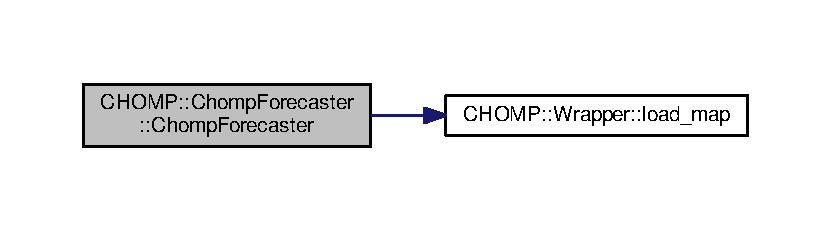
\includegraphics[width=350pt]{class_c_h_o_m_p_1_1_chomp_forecaster_a58176b34170de8485029f182e05f12c5_cgraph}
\end{center}
\end{figure}




\subsection{Member Function Documentation}
\index{C\+H\+O\+M\+P\+::\+Chomp\+Forecaster@{C\+H\+O\+M\+P\+::\+Chomp\+Forecaster}!callback\+\_\+target\+\_\+state@{callback\+\_\+target\+\_\+state}}
\index{callback\+\_\+target\+\_\+state@{callback\+\_\+target\+\_\+state}!C\+H\+O\+M\+P\+::\+Chomp\+Forecaster@{C\+H\+O\+M\+P\+::\+Chomp\+Forecaster}}
\subsubsection[{\texorpdfstring{callback\+\_\+target\+\_\+state(geometry\+\_\+msgs\+::\+Pose\+Stamped\+Const\+Ptr pose\+\_\+stamped\+\_\+ptr)}{callback_target_state(geometry_msgs::PoseStampedConstPtr pose_stamped_ptr)}}]{\setlength{\rightskip}{0pt plus 5cm}void Chomp\+Forecaster\+::callback\+\_\+target\+\_\+state (
\begin{DoxyParamCaption}
\item[{geometry\+\_\+msgs\+::\+Pose\+Stamped\+Const\+Ptr}]{pose\+\_\+stamped\+\_\+ptr}
\end{DoxyParamCaption}
)}\hypertarget{class_c_h_o_m_p_1_1_chomp_forecaster_ac05e634464c8859c8cc3e8bdb1a40ded}{}\label{class_c_h_o_m_p_1_1_chomp_forecaster_ac05e634464c8859c8cc3e8bdb1a40ded}


Definition at line 248 of file chomp\+\_\+predict.\+cpp.



Here is the call graph for this function\+:\nopagebreak
\begin{figure}[H]
\begin{center}
\leavevmode
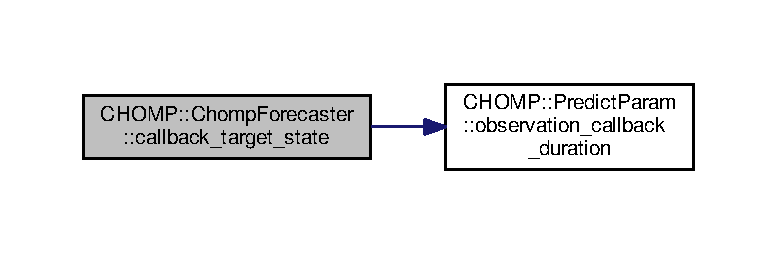
\includegraphics[width=350pt]{class_c_h_o_m_p_1_1_chomp_forecaster_ac05e634464c8859c8cc3e8bdb1a40ded_cgraph}
\end{center}
\end{figure}




Here is the caller graph for this function\+:
\nopagebreak
\begin{figure}[H]
\begin{center}
\leavevmode
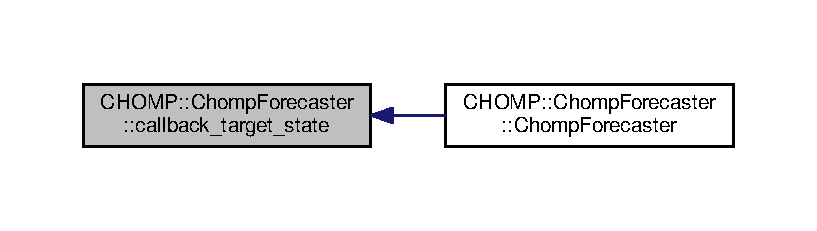
\includegraphics[width=350pt]{class_c_h_o_m_p_1_1_chomp_forecaster_ac05e634464c8859c8cc3e8bdb1a40ded_icgraph}
\end{center}
\end{figure}


\index{C\+H\+O\+M\+P\+::\+Chomp\+Forecaster@{C\+H\+O\+M\+P\+::\+Chomp\+Forecaster}!eval\+\_\+prediction@{eval\+\_\+prediction}}
\index{eval\+\_\+prediction@{eval\+\_\+prediction}!C\+H\+O\+M\+P\+::\+Chomp\+Forecaster@{C\+H\+O\+M\+P\+::\+Chomp\+Forecaster}}
\subsubsection[{\texorpdfstring{eval\+\_\+prediction(ros\+::\+Time eval\+\_\+time)}{eval_prediction(ros::Time eval_time)}}]{\setlength{\rightskip}{0pt plus 5cm}geometry\+\_\+msgs\+::\+Point Chomp\+Forecaster\+::eval\+\_\+prediction (
\begin{DoxyParamCaption}
\item[{ros\+::\+Time}]{eval\+\_\+time}
\end{DoxyParamCaption}
)}\hypertarget{class_c_h_o_m_p_1_1_chomp_forecaster_a8b3e5ea0d8a5092b371a23efcddd5c73}{}\label{class_c_h_o_m_p_1_1_chomp_forecaster_a8b3e5ea0d8a5092b371a23efcddd5c73}


Once prediction model is acquired, then we can evaluate the prediction in time. 


\begin{DoxyParams}{Parameters}
{\em eval\+\_\+time} & \\
\hline
\end{DoxyParams}
\begin{DoxyReturn}{Returns}
geometry\+\_\+msgs\+::\+Point 
\end{DoxyReturn}


Definition at line 388 of file chomp\+\_\+predict.\+cpp.



Here is the call graph for this function\+:
\nopagebreak
\begin{figure}[H]
\begin{center}
\leavevmode
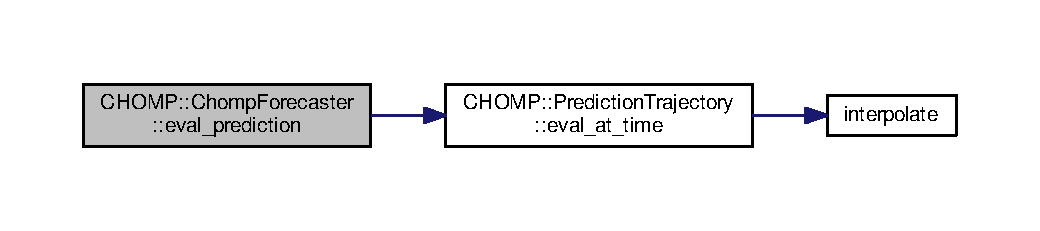
\includegraphics[width=350pt]{class_c_h_o_m_p_1_1_chomp_forecaster_a8b3e5ea0d8a5092b371a23efcddd5c73_cgraph}
\end{center}
\end{figure}




Here is the caller graph for this function\+:
\nopagebreak
\begin{figure}[H]
\begin{center}
\leavevmode
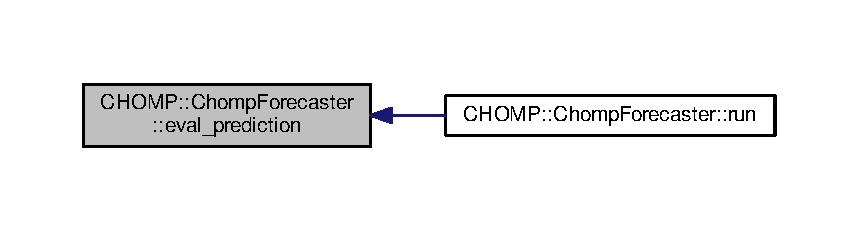
\includegraphics[width=350pt]{class_c_h_o_m_p_1_1_chomp_forecaster_a8b3e5ea0d8a5092b371a23efcddd5c73_icgraph}
\end{center}
\end{figure}


\index{C\+H\+O\+M\+P\+::\+Chomp\+Forecaster@{C\+H\+O\+M\+P\+::\+Chomp\+Forecaster}!predict\+\_\+with\+\_\+obsrv\+\_\+queue@{predict\+\_\+with\+\_\+obsrv\+\_\+queue}}
\index{predict\+\_\+with\+\_\+obsrv\+\_\+queue@{predict\+\_\+with\+\_\+obsrv\+\_\+queue}!C\+H\+O\+M\+P\+::\+Chomp\+Forecaster@{C\+H\+O\+M\+P\+::\+Chomp\+Forecaster}}
\subsubsection[{\texorpdfstring{predict\+\_\+with\+\_\+obsrv\+\_\+queue()}{predict_with_obsrv_queue()}}]{\setlength{\rightskip}{0pt plus 5cm}void Chomp\+Forecaster\+::predict\+\_\+with\+\_\+obsrv\+\_\+queue (
\begin{DoxyParamCaption}
{}
\end{DoxyParamCaption}
)}\hypertarget{class_c_h_o_m_p_1_1_chomp_forecaster_a02a3930b78aaf72a9058cb3ce6ae8143}{}\label{class_c_h_o_m_p_1_1_chomp_forecaster_a02a3930b78aaf72a9058cb3ce6ae8143}


Definition at line 272 of file chomp\+\_\+predict.\+cpp.



Here is the call graph for this function\+:
\nopagebreak
\begin{figure}[H]
\begin{center}
\leavevmode
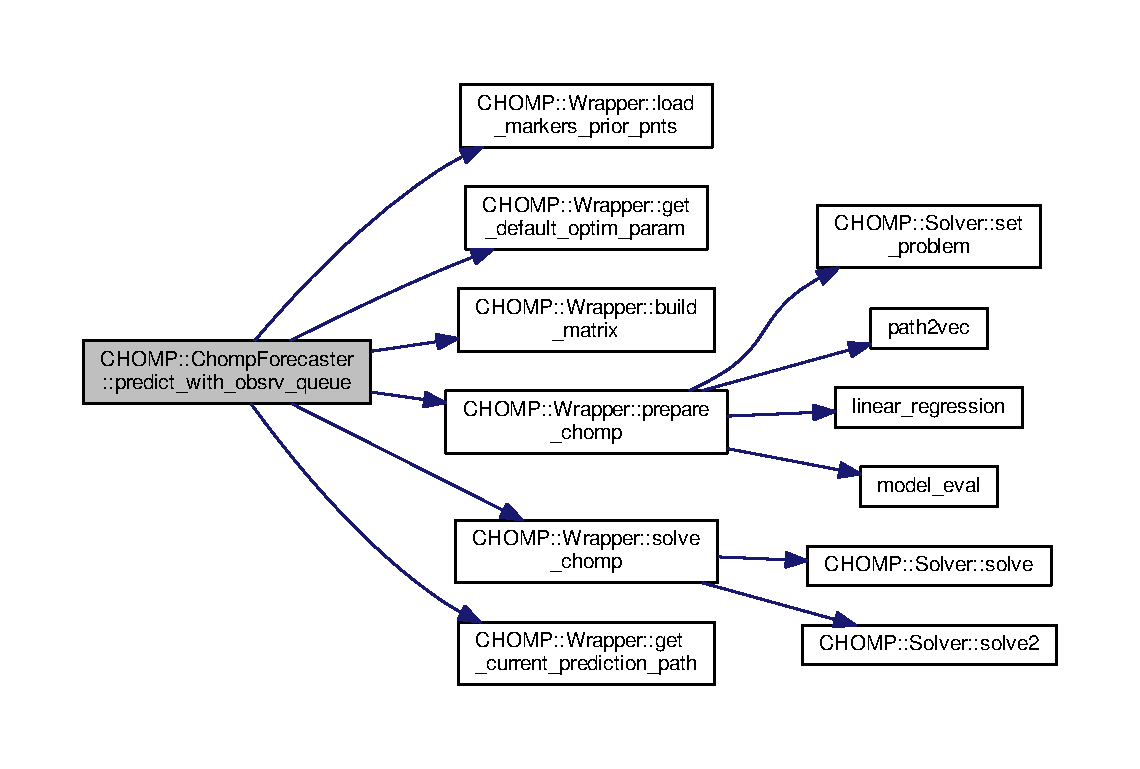
\includegraphics[width=350pt]{class_c_h_o_m_p_1_1_chomp_forecaster_a02a3930b78aaf72a9058cb3ce6ae8143_cgraph}
\end{center}
\end{figure}




Here is the caller graph for this function\+:
\nopagebreak
\begin{figure}[H]
\begin{center}
\leavevmode
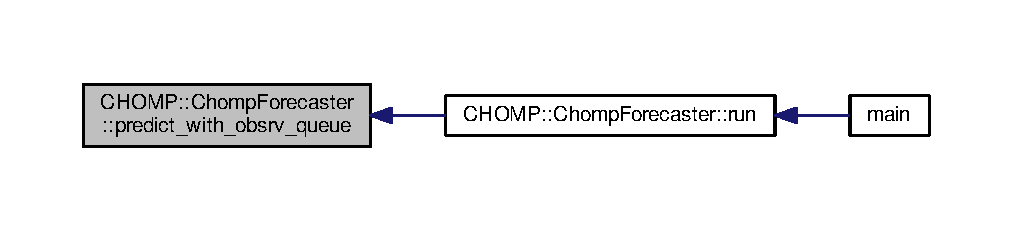
\includegraphics[width=350pt]{class_c_h_o_m_p_1_1_chomp_forecaster_a02a3930b78aaf72a9058cb3ce6ae8143_icgraph}
\end{center}
\end{figure}


\index{C\+H\+O\+M\+P\+::\+Chomp\+Forecaster@{C\+H\+O\+M\+P\+::\+Chomp\+Forecaster}!publish\+\_\+routine@{publish\+\_\+routine}}
\index{publish\+\_\+routine@{publish\+\_\+routine}!C\+H\+O\+M\+P\+::\+Chomp\+Forecaster@{C\+H\+O\+M\+P\+::\+Chomp\+Forecaster}}
\subsubsection[{\texorpdfstring{publish\+\_\+routine()}{publish_routine()}}]{\setlength{\rightskip}{0pt plus 5cm}void Chomp\+Forecaster\+::publish\+\_\+routine (
\begin{DoxyParamCaption}
{}
\end{DoxyParamCaption}
)}\hypertarget{class_c_h_o_m_p_1_1_chomp_forecaster_a56e9984f3c85563170c58708aaa97056}{}\label{class_c_h_o_m_p_1_1_chomp_forecaster_a56e9984f3c85563170c58708aaa97056}


publish routine in while loop 

/ 2. observation queue / 3.\+prediction path during prediction horizon (not entire path) 

Definition at line 319 of file chomp\+\_\+predict.\+cpp.



Here is the caller graph for this function\+:
\nopagebreak
\begin{figure}[H]
\begin{center}
\leavevmode
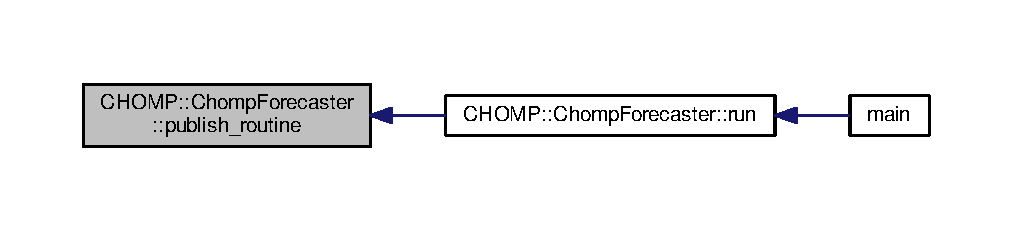
\includegraphics[width=350pt]{class_c_h_o_m_p_1_1_chomp_forecaster_a56e9984f3c85563170c58708aaa97056_icgraph}
\end{center}
\end{figure}


\index{C\+H\+O\+M\+P\+::\+Chomp\+Forecaster@{C\+H\+O\+M\+P\+::\+Chomp\+Forecaster}!run@{run}}
\index{run@{run}!C\+H\+O\+M\+P\+::\+Chomp\+Forecaster@{C\+H\+O\+M\+P\+::\+Chomp\+Forecaster}}
\subsubsection[{\texorpdfstring{run()}{run()}}]{\setlength{\rightskip}{0pt plus 5cm}void Chomp\+Forecaster\+::run (
\begin{DoxyParamCaption}
{}
\end{DoxyParamCaption}
)}\hypertarget{class_c_h_o_m_p_1_1_chomp_forecaster_af225bf2af3fede364b922e27be410f0b}{}\label{class_c_h_o_m_p_1_1_chomp_forecaster_af225bf2af3fede364b922e27be410f0b}


code to be run in the main loop 



Definition at line 332 of file chomp\+\_\+predict.\+cpp.



Here is the call graph for this function\+:
\nopagebreak
\begin{figure}[H]
\begin{center}
\leavevmode
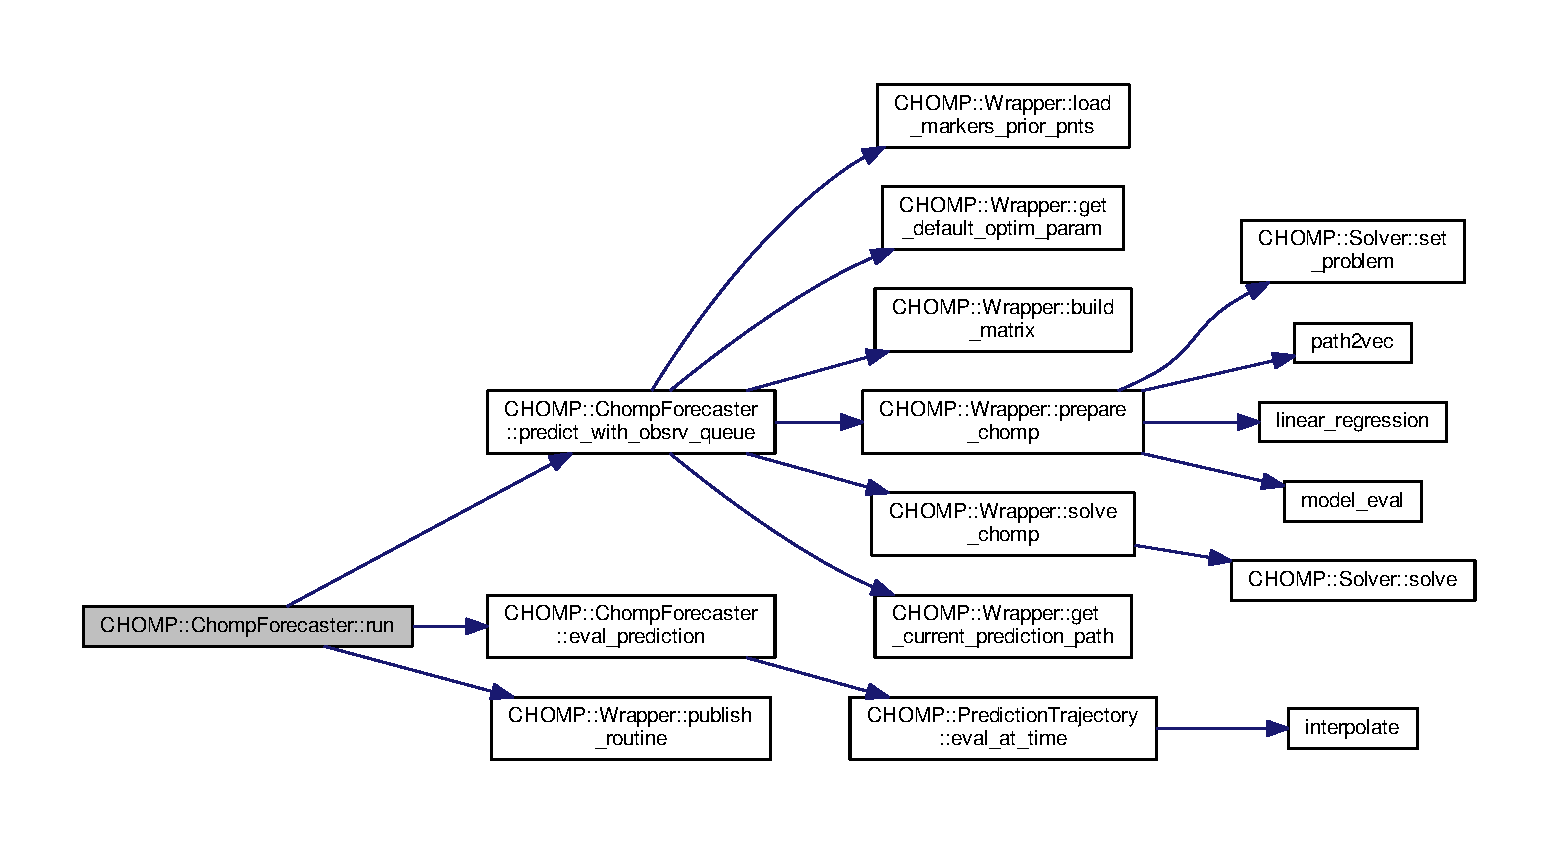
\includegraphics[width=350pt]{class_c_h_o_m_p_1_1_chomp_forecaster_af225bf2af3fede364b922e27be410f0b_cgraph}
\end{center}
\end{figure}




Here is the caller graph for this function\+:
\nopagebreak
\begin{figure}[H]
\begin{center}
\leavevmode
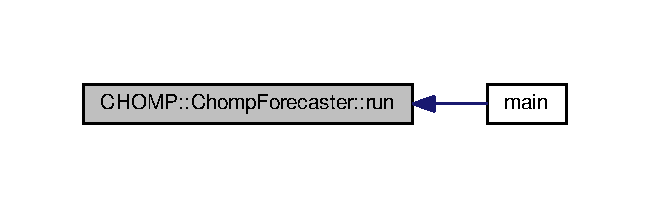
\includegraphics[width=312pt]{class_c_h_o_m_p_1_1_chomp_forecaster_af225bf2af3fede364b922e27be410f0b_icgraph}
\end{center}
\end{figure}




\subsection{Member Data Documentation}
\index{C\+H\+O\+M\+P\+::\+Chomp\+Forecaster@{C\+H\+O\+M\+P\+::\+Chomp\+Forecaster}!is\+\_\+predicted@{is\+\_\+predicted}}
\index{is\+\_\+predicted@{is\+\_\+predicted}!C\+H\+O\+M\+P\+::\+Chomp\+Forecaster@{C\+H\+O\+M\+P\+::\+Chomp\+Forecaster}}
\subsubsection[{\texorpdfstring{is\+\_\+predicted}{is_predicted}}]{\setlength{\rightskip}{0pt plus 5cm}bool C\+H\+O\+M\+P\+::\+Chomp\+Forecaster\+::is\+\_\+predicted}\hypertarget{class_c_h_o_m_p_1_1_chomp_forecaster_ae092aa988e2587db915e287fc3fa0aff}{}\label{class_c_h_o_m_p_1_1_chomp_forecaster_ae092aa988e2587db915e287fc3fa0aff}


Definition at line 81 of file chomp\+\_\+predict.\+h.

\index{C\+H\+O\+M\+P\+::\+Chomp\+Forecaster@{C\+H\+O\+M\+P\+::\+Chomp\+Forecaster}!is\+\_\+state\+\_\+received@{is\+\_\+state\+\_\+received}}
\index{is\+\_\+state\+\_\+received@{is\+\_\+state\+\_\+received}!C\+H\+O\+M\+P\+::\+Chomp\+Forecaster@{C\+H\+O\+M\+P\+::\+Chomp\+Forecaster}}
\subsubsection[{\texorpdfstring{is\+\_\+state\+\_\+received}{is_state_received}}]{\setlength{\rightskip}{0pt plus 5cm}bool C\+H\+O\+M\+P\+::\+Chomp\+Forecaster\+::is\+\_\+state\+\_\+received}\hypertarget{class_c_h_o_m_p_1_1_chomp_forecaster_ae642d133970543c83eebd153d74e8459}{}\label{class_c_h_o_m_p_1_1_chomp_forecaster_ae642d133970543c83eebd153d74e8459}


Definition at line 80 of file chomp\+\_\+predict.\+h.



The documentation for this class was generated from the following files\+:\begin{DoxyCompactItemize}
\item 
include/chomp\+\_\+predict/\hyperlink{chomp__predict_8h}{chomp\+\_\+predict.\+h}\item 
src/\hyperlink{chomp__predict_8cpp}{chomp\+\_\+predict.\+cpp}\end{DoxyCompactItemize}

\hypertarget{struct_c_h_o_m_p_1_1_cost_param}{}\section{C\+H\+O\+MP\+:\+:Cost\+Param Struct Reference}
\label{struct_c_h_o_m_p_1_1_cost_param}\index{C\+H\+O\+M\+P\+::\+Cost\+Param@{C\+H\+O\+M\+P\+::\+Cost\+Param}}


{\ttfamily \#include $<$chomp\+\_\+subroutine.\+h$>$}

\subsection*{Public Attributes}
\begin{DoxyCompactItemize}
\item 
double \hyperlink{struct_c_h_o_m_p_1_1_cost_param_a9ab5a375539e209151d57dea31b4eed9}{r\+\_\+safe}
\item 
double \hyperlink{struct_c_h_o_m_p_1_1_cost_param_aac37a7ec506745fea119ff57a711b0b6}{dx}
\item 
double \hyperlink{struct_c_h_o_m_p_1_1_cost_param_afdb481a80ee8ef47dc837075993f0821}{ground\+\_\+height}
\end{DoxyCompactItemize}


\subsection{Detailed Description}


Definition at line 53 of file chomp\+\_\+subroutine.\+h.



\subsection{Member Data Documentation}
\index{C\+H\+O\+M\+P\+::\+Cost\+Param@{C\+H\+O\+M\+P\+::\+Cost\+Param}!dx@{dx}}
\index{dx@{dx}!C\+H\+O\+M\+P\+::\+Cost\+Param@{C\+H\+O\+M\+P\+::\+Cost\+Param}}
\subsubsection[{\texorpdfstring{dx}{dx}}]{\setlength{\rightskip}{0pt plus 5cm}double C\+H\+O\+M\+P\+::\+Cost\+Param\+::dx}\hypertarget{struct_c_h_o_m_p_1_1_cost_param_aac37a7ec506745fea119ff57a711b0b6}{}\label{struct_c_h_o_m_p_1_1_cost_param_aac37a7ec506745fea119ff57a711b0b6}


Definition at line 55 of file chomp\+\_\+subroutine.\+h.

\index{C\+H\+O\+M\+P\+::\+Cost\+Param@{C\+H\+O\+M\+P\+::\+Cost\+Param}!ground\+\_\+height@{ground\+\_\+height}}
\index{ground\+\_\+height@{ground\+\_\+height}!C\+H\+O\+M\+P\+::\+Cost\+Param@{C\+H\+O\+M\+P\+::\+Cost\+Param}}
\subsubsection[{\texorpdfstring{ground\+\_\+height}{ground_height}}]{\setlength{\rightskip}{0pt plus 5cm}double C\+H\+O\+M\+P\+::\+Cost\+Param\+::ground\+\_\+height}\hypertarget{struct_c_h_o_m_p_1_1_cost_param_afdb481a80ee8ef47dc837075993f0821}{}\label{struct_c_h_o_m_p_1_1_cost_param_afdb481a80ee8ef47dc837075993f0821}


Definition at line 56 of file chomp\+\_\+subroutine.\+h.

\index{C\+H\+O\+M\+P\+::\+Cost\+Param@{C\+H\+O\+M\+P\+::\+Cost\+Param}!r\+\_\+safe@{r\+\_\+safe}}
\index{r\+\_\+safe@{r\+\_\+safe}!C\+H\+O\+M\+P\+::\+Cost\+Param@{C\+H\+O\+M\+P\+::\+Cost\+Param}}
\subsubsection[{\texorpdfstring{r\+\_\+safe}{r_safe}}]{\setlength{\rightskip}{0pt plus 5cm}double C\+H\+O\+M\+P\+::\+Cost\+Param\+::r\+\_\+safe}\hypertarget{struct_c_h_o_m_p_1_1_cost_param_a9ab5a375539e209151d57dea31b4eed9}{}\label{struct_c_h_o_m_p_1_1_cost_param_a9ab5a375539e209151d57dea31b4eed9}


Definition at line 54 of file chomp\+\_\+subroutine.\+h.



The documentation for this struct was generated from the following file\+:\begin{DoxyCompactItemize}
\item 
include/chomp\+\_\+predict/\hyperlink{chomp__subroutine_8h}{chomp\+\_\+subroutine.\+h}\end{DoxyCompactItemize}

\hypertarget{struct_linear_model}{}\section{Linear\+Model Struct Reference}
\label{struct_linear_model}\index{Linear\+Model@{Linear\+Model}}


{\ttfamily \#include $<$chomp\+\_\+utils.\+h$>$}

\subsection*{Public Attributes}
\begin{DoxyCompactItemize}
\item 
double \hyperlink{struct_linear_model_ae49f43f205d39ee14841dae7f83abab4}{beta0}
\item 
double \hyperlink{struct_linear_model_af8db55999999e4adb71ddc1883297e4c}{beta1}
\end{DoxyCompactItemize}


\subsection{Detailed Description}


Definition at line 19 of file chomp\+\_\+utils.\+h.



\subsection{Member Data Documentation}
\index{Linear\+Model@{Linear\+Model}!beta0@{beta0}}
\index{beta0@{beta0}!Linear\+Model@{Linear\+Model}}
\subsubsection[{\texorpdfstring{beta0}{beta0}}]{\setlength{\rightskip}{0pt plus 5cm}double Linear\+Model\+::beta0}\hypertarget{struct_linear_model_ae49f43f205d39ee14841dae7f83abab4}{}\label{struct_linear_model_ae49f43f205d39ee14841dae7f83abab4}


Definition at line 21 of file chomp\+\_\+utils.\+h.

\index{Linear\+Model@{Linear\+Model}!beta1@{beta1}}
\index{beta1@{beta1}!Linear\+Model@{Linear\+Model}}
\subsubsection[{\texorpdfstring{beta1}{beta1}}]{\setlength{\rightskip}{0pt plus 5cm}double Linear\+Model\+::beta1}\hypertarget{struct_linear_model_af8db55999999e4adb71ddc1883297e4c}{}\label{struct_linear_model_af8db55999999e4adb71ddc1883297e4c}


Definition at line 22 of file chomp\+\_\+utils.\+h.



The documentation for this struct was generated from the following file\+:\begin{DoxyCompactItemize}
\item 
include/\hyperlink{chomp__utils_8h}{chomp\+\_\+utils.\+h}\end{DoxyCompactItemize}

\hypertarget{struct_c_h_o_m_p_1_1_optim_info}{}\section{C\+H\+O\+MP\+:\+:Optim\+Info Struct Reference}
\label{struct_c_h_o_m_p_1_1_optim_info}\index{C\+H\+O\+M\+P\+::\+Optim\+Info@{C\+H\+O\+M\+P\+::\+Optim\+Info}}


{\ttfamily \#include $<$chomp\+\_\+subroutine.\+h$>$}

\subsection*{Public Attributes}
\begin{DoxyCompactItemize}
\item 
vector$<$ double $>$ \hyperlink{struct_c_h_o_m_p_1_1_optim_info_af3837487472aa772f6aeace2c32f356a}{prior\+\_\+cost\+\_\+history}
\item 
vector$<$ double $>$ \hyperlink{struct_c_h_o_m_p_1_1_optim_info_a80f485a174b1213d23e2c378ebcbafe2}{nonlinear\+\_\+cost\+\_\+history}
\item 
vector$<$ double $>$ \hyperlink{struct_c_h_o_m_p_1_1_optim_info_a47f69044821c9ff79aabd1acb5424926}{total\+\_\+cost\+\_\+history}
\end{DoxyCompactItemize}


\subsection{Detailed Description}


Definition at line 37 of file chomp\+\_\+subroutine.\+h.



\subsection{Member Data Documentation}
\index{C\+H\+O\+M\+P\+::\+Optim\+Info@{C\+H\+O\+M\+P\+::\+Optim\+Info}!nonlinear\+\_\+cost\+\_\+history@{nonlinear\+\_\+cost\+\_\+history}}
\index{nonlinear\+\_\+cost\+\_\+history@{nonlinear\+\_\+cost\+\_\+history}!C\+H\+O\+M\+P\+::\+Optim\+Info@{C\+H\+O\+M\+P\+::\+Optim\+Info}}
\subsubsection[{\texorpdfstring{nonlinear\+\_\+cost\+\_\+history}{nonlinear_cost_history}}]{\setlength{\rightskip}{0pt plus 5cm}vector$<$double$>$ C\+H\+O\+M\+P\+::\+Optim\+Info\+::nonlinear\+\_\+cost\+\_\+history}\hypertarget{struct_c_h_o_m_p_1_1_optim_info_a80f485a174b1213d23e2c378ebcbafe2}{}\label{struct_c_h_o_m_p_1_1_optim_info_a80f485a174b1213d23e2c378ebcbafe2}


Definition at line 39 of file chomp\+\_\+subroutine.\+h.

\index{C\+H\+O\+M\+P\+::\+Optim\+Info@{C\+H\+O\+M\+P\+::\+Optim\+Info}!prior\+\_\+cost\+\_\+history@{prior\+\_\+cost\+\_\+history}}
\index{prior\+\_\+cost\+\_\+history@{prior\+\_\+cost\+\_\+history}!C\+H\+O\+M\+P\+::\+Optim\+Info@{C\+H\+O\+M\+P\+::\+Optim\+Info}}
\subsubsection[{\texorpdfstring{prior\+\_\+cost\+\_\+history}{prior_cost_history}}]{\setlength{\rightskip}{0pt plus 5cm}vector$<$double$>$ C\+H\+O\+M\+P\+::\+Optim\+Info\+::prior\+\_\+cost\+\_\+history}\hypertarget{struct_c_h_o_m_p_1_1_optim_info_af3837487472aa772f6aeace2c32f356a}{}\label{struct_c_h_o_m_p_1_1_optim_info_af3837487472aa772f6aeace2c32f356a}


Definition at line 38 of file chomp\+\_\+subroutine.\+h.

\index{C\+H\+O\+M\+P\+::\+Optim\+Info@{C\+H\+O\+M\+P\+::\+Optim\+Info}!total\+\_\+cost\+\_\+history@{total\+\_\+cost\+\_\+history}}
\index{total\+\_\+cost\+\_\+history@{total\+\_\+cost\+\_\+history}!C\+H\+O\+M\+P\+::\+Optim\+Info@{C\+H\+O\+M\+P\+::\+Optim\+Info}}
\subsubsection[{\texorpdfstring{total\+\_\+cost\+\_\+history}{total_cost_history}}]{\setlength{\rightskip}{0pt plus 5cm}vector$<$double$>$ C\+H\+O\+M\+P\+::\+Optim\+Info\+::total\+\_\+cost\+\_\+history}\hypertarget{struct_c_h_o_m_p_1_1_optim_info_a47f69044821c9ff79aabd1acb5424926}{}\label{struct_c_h_o_m_p_1_1_optim_info_a47f69044821c9ff79aabd1acb5424926}


Definition at line 40 of file chomp\+\_\+subroutine.\+h.



The documentation for this struct was generated from the following file\+:\begin{DoxyCompactItemize}
\item 
include/chomp\+\_\+predict/\hyperlink{chomp__subroutine_8h}{chomp\+\_\+subroutine.\+h}\end{DoxyCompactItemize}

\hypertarget{struct_c_h_o_m_p_1_1_optim_param}{}\section{C\+H\+O\+MP\+:\+:Optim\+Param Struct Reference}
\label{struct_c_h_o_m_p_1_1_optim_param}\index{C\+H\+O\+M\+P\+::\+Optim\+Param@{C\+H\+O\+M\+P\+::\+Optim\+Param}}


{\ttfamily \#include $<$chomp\+\_\+subroutine.\+h$>$}

\subsection*{Public Attributes}
\begin{DoxyCompactItemize}
\item 
int \hyperlink{struct_c_h_o_m_p_1_1_optim_param_a0ede8f165be67dd3607e47fa90ed9c31}{max\+\_\+iter}
\item 
double \hyperlink{struct_c_h_o_m_p_1_1_optim_param_afb3b23647f1698f1815f4f877ac302ea}{termination\+\_\+cond}
\item 
double \hyperlink{struct_c_h_o_m_p_1_1_optim_param_a24f769bd28ca6ecceadb0b88a6e5c8fa}{descending\+\_\+rate}
\item 
double \hyperlink{struct_c_h_o_m_p_1_1_optim_param_a7dc4e45cd704217867a399e656af6b87}{weight\+\_\+prior}
\item 
double \hyperlink{struct_c_h_o_m_p_1_1_optim_param_a08dbedf3d695dd849e99972eeda4854a}{gamma}
\item 
int \hyperlink{struct_c_h_o_m_p_1_1_optim_param_ac6dafdf330d8f879009f461a77b41c63}{n\+\_\+step}
\end{DoxyCompactItemize}


\subsection{Detailed Description}


Definition at line 27 of file chomp\+\_\+subroutine.\+h.



\subsection{Member Data Documentation}
\index{C\+H\+O\+M\+P\+::\+Optim\+Param@{C\+H\+O\+M\+P\+::\+Optim\+Param}!descending\+\_\+rate@{descending\+\_\+rate}}
\index{descending\+\_\+rate@{descending\+\_\+rate}!C\+H\+O\+M\+P\+::\+Optim\+Param@{C\+H\+O\+M\+P\+::\+Optim\+Param}}
\subsubsection[{\texorpdfstring{descending\+\_\+rate}{descending_rate}}]{\setlength{\rightskip}{0pt plus 5cm}double C\+H\+O\+M\+P\+::\+Optim\+Param\+::descending\+\_\+rate}\hypertarget{struct_c_h_o_m_p_1_1_optim_param_a24f769bd28ca6ecceadb0b88a6e5c8fa}{}\label{struct_c_h_o_m_p_1_1_optim_param_a24f769bd28ca6ecceadb0b88a6e5c8fa}


Definition at line 30 of file chomp\+\_\+subroutine.\+h.

\index{C\+H\+O\+M\+P\+::\+Optim\+Param@{C\+H\+O\+M\+P\+::\+Optim\+Param}!gamma@{gamma}}
\index{gamma@{gamma}!C\+H\+O\+M\+P\+::\+Optim\+Param@{C\+H\+O\+M\+P\+::\+Optim\+Param}}
\subsubsection[{\texorpdfstring{gamma}{gamma}}]{\setlength{\rightskip}{0pt plus 5cm}double C\+H\+O\+M\+P\+::\+Optim\+Param\+::gamma}\hypertarget{struct_c_h_o_m_p_1_1_optim_param_a08dbedf3d695dd849e99972eeda4854a}{}\label{struct_c_h_o_m_p_1_1_optim_param_a08dbedf3d695dd849e99972eeda4854a}


Definition at line 32 of file chomp\+\_\+subroutine.\+h.

\index{C\+H\+O\+M\+P\+::\+Optim\+Param@{C\+H\+O\+M\+P\+::\+Optim\+Param}!max\+\_\+iter@{max\+\_\+iter}}
\index{max\+\_\+iter@{max\+\_\+iter}!C\+H\+O\+M\+P\+::\+Optim\+Param@{C\+H\+O\+M\+P\+::\+Optim\+Param}}
\subsubsection[{\texorpdfstring{max\+\_\+iter}{max_iter}}]{\setlength{\rightskip}{0pt plus 5cm}int C\+H\+O\+M\+P\+::\+Optim\+Param\+::max\+\_\+iter}\hypertarget{struct_c_h_o_m_p_1_1_optim_param_a0ede8f165be67dd3607e47fa90ed9c31}{}\label{struct_c_h_o_m_p_1_1_optim_param_a0ede8f165be67dd3607e47fa90ed9c31}


Definition at line 28 of file chomp\+\_\+subroutine.\+h.

\index{C\+H\+O\+M\+P\+::\+Optim\+Param@{C\+H\+O\+M\+P\+::\+Optim\+Param}!n\+\_\+step@{n\+\_\+step}}
\index{n\+\_\+step@{n\+\_\+step}!C\+H\+O\+M\+P\+::\+Optim\+Param@{C\+H\+O\+M\+P\+::\+Optim\+Param}}
\subsubsection[{\texorpdfstring{n\+\_\+step}{n_step}}]{\setlength{\rightskip}{0pt plus 5cm}int C\+H\+O\+M\+P\+::\+Optim\+Param\+::n\+\_\+step}\hypertarget{struct_c_h_o_m_p_1_1_optim_param_ac6dafdf330d8f879009f461a77b41c63}{}\label{struct_c_h_o_m_p_1_1_optim_param_ac6dafdf330d8f879009f461a77b41c63}


Definition at line 33 of file chomp\+\_\+subroutine.\+h.

\index{C\+H\+O\+M\+P\+::\+Optim\+Param@{C\+H\+O\+M\+P\+::\+Optim\+Param}!termination\+\_\+cond@{termination\+\_\+cond}}
\index{termination\+\_\+cond@{termination\+\_\+cond}!C\+H\+O\+M\+P\+::\+Optim\+Param@{C\+H\+O\+M\+P\+::\+Optim\+Param}}
\subsubsection[{\texorpdfstring{termination\+\_\+cond}{termination_cond}}]{\setlength{\rightskip}{0pt plus 5cm}double C\+H\+O\+M\+P\+::\+Optim\+Param\+::termination\+\_\+cond}\hypertarget{struct_c_h_o_m_p_1_1_optim_param_afb3b23647f1698f1815f4f877ac302ea}{}\label{struct_c_h_o_m_p_1_1_optim_param_afb3b23647f1698f1815f4f877ac302ea}


Definition at line 29 of file chomp\+\_\+subroutine.\+h.

\index{C\+H\+O\+M\+P\+::\+Optim\+Param@{C\+H\+O\+M\+P\+::\+Optim\+Param}!weight\+\_\+prior@{weight\+\_\+prior}}
\index{weight\+\_\+prior@{weight\+\_\+prior}!C\+H\+O\+M\+P\+::\+Optim\+Param@{C\+H\+O\+M\+P\+::\+Optim\+Param}}
\subsubsection[{\texorpdfstring{weight\+\_\+prior}{weight_prior}}]{\setlength{\rightskip}{0pt plus 5cm}double C\+H\+O\+M\+P\+::\+Optim\+Param\+::weight\+\_\+prior}\hypertarget{struct_c_h_o_m_p_1_1_optim_param_a7dc4e45cd704217867a399e656af6b87}{}\label{struct_c_h_o_m_p_1_1_optim_param_a7dc4e45cd704217867a399e656af6b87}


Definition at line 31 of file chomp\+\_\+subroutine.\+h.



The documentation for this struct was generated from the following file\+:\begin{DoxyCompactItemize}
\item 
include/chomp\+\_\+predict/\hyperlink{chomp__subroutine_8h}{chomp\+\_\+subroutine.\+h}\end{DoxyCompactItemize}

\hypertarget{struct_c_h_o_m_p_1_1_optim_result}{}\section{C\+H\+O\+MP\+:\+:Optim\+Result Struct Reference}
\label{struct_c_h_o_m_p_1_1_optim_result}\index{C\+H\+O\+M\+P\+::\+Optim\+Result@{C\+H\+O\+M\+P\+::\+Optim\+Result}}


{\ttfamily \#include $<$chomp\+\_\+subroutine.\+h$>$}



Collaboration diagram for C\+H\+O\+MP\+:\+:Optim\+Result\+:\nopagebreak
\begin{figure}[H]
\begin{center}
\leavevmode
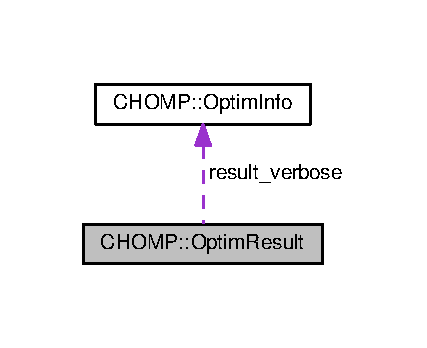
\includegraphics[width=205pt]{struct_c_h_o_m_p_1_1_optim_result__coll__graph}
\end{center}
\end{figure}
\subsection*{Public Attributes}
\begin{DoxyCompactItemize}
\item 
\hyperlink{struct_c_h_o_m_p_1_1_optim_info}{Optim\+Info} \hyperlink{struct_c_h_o_m_p_1_1_optim_result_aa4314b8ae0ca38f9bad7fd8c7e1f9492}{result\+\_\+verbose}
\item 
Eigen\+::\+Vector\+Xd \hyperlink{struct_c_h_o_m_p_1_1_optim_result_ae85f14f34c231bb2f5767553b6771f9c}{solution}
\end{DoxyCompactItemize}


\subsection{Detailed Description}


Definition at line 44 of file chomp\+\_\+subroutine.\+h.



\subsection{Member Data Documentation}
\index{C\+H\+O\+M\+P\+::\+Optim\+Result@{C\+H\+O\+M\+P\+::\+Optim\+Result}!result\+\_\+verbose@{result\+\_\+verbose}}
\index{result\+\_\+verbose@{result\+\_\+verbose}!C\+H\+O\+M\+P\+::\+Optim\+Result@{C\+H\+O\+M\+P\+::\+Optim\+Result}}
\subsubsection[{\texorpdfstring{result\+\_\+verbose}{result_verbose}}]{\setlength{\rightskip}{0pt plus 5cm}{\bf Optim\+Info} C\+H\+O\+M\+P\+::\+Optim\+Result\+::result\+\_\+verbose}\hypertarget{struct_c_h_o_m_p_1_1_optim_result_aa4314b8ae0ca38f9bad7fd8c7e1f9492}{}\label{struct_c_h_o_m_p_1_1_optim_result_aa4314b8ae0ca38f9bad7fd8c7e1f9492}


Definition at line 45 of file chomp\+\_\+subroutine.\+h.

\index{C\+H\+O\+M\+P\+::\+Optim\+Result@{C\+H\+O\+M\+P\+::\+Optim\+Result}!solution@{solution}}
\index{solution@{solution}!C\+H\+O\+M\+P\+::\+Optim\+Result@{C\+H\+O\+M\+P\+::\+Optim\+Result}}
\subsubsection[{\texorpdfstring{solution}{solution}}]{\setlength{\rightskip}{0pt plus 5cm}Eigen\+::\+Vector\+Xd C\+H\+O\+M\+P\+::\+Optim\+Result\+::solution}\hypertarget{struct_c_h_o_m_p_1_1_optim_result_ae85f14f34c231bb2f5767553b6771f9c}{}\label{struct_c_h_o_m_p_1_1_optim_result_ae85f14f34c231bb2f5767553b6771f9c}


Definition at line 46 of file chomp\+\_\+subroutine.\+h.



The documentation for this struct was generated from the following file\+:\begin{DoxyCompactItemize}
\item 
include/chomp\+\_\+predict/\hyperlink{chomp__subroutine_8h}{chomp\+\_\+subroutine.\+h}\end{DoxyCompactItemize}

\hypertarget{struct_c_h_o_m_p_1_1_prediction_trajectory}{}\section{C\+H\+O\+MP\+:\+:Prediction\+Trajectory Struct Reference}
\label{struct_c_h_o_m_p_1_1_prediction_trajectory}\index{C\+H\+O\+M\+P\+::\+Prediction\+Trajectory@{C\+H\+O\+M\+P\+::\+Prediction\+Trajectory}}


{\ttfamily \#include $<$chomp\+\_\+predict.\+h$>$}

\subsection*{Public Member Functions}
\begin{DoxyCompactItemize}
\item 
\hyperlink{struct_c_h_o_m_p_1_1_prediction_trajectory_a51c4006f1e9ba69099e06b9052a14a1d}{Prediction\+Trajectory} ()
\item 
\hyperlink{struct_c_h_o_m_p_1_1_prediction_trajectory_aac8376bbb1a9b75bf87811fbcec6d062}{Prediction\+Trajectory} (Vector\+Xd obsrv\+\_\+time\+\_\+seq, Matrix\+Xd path)
\begin{DoxyCompactList}\small\item\em Construct a new Prediction Trajectory object. Also complete a prediction traj directly from observation traj and future path predicton. \end{DoxyCompactList}\item 
Vector3d \hyperlink{struct_c_h_o_m_p_1_1_prediction_trajectory_a3e50b3be07e9531449128eae47c60442}{eval\+\_\+at\+\_\+time} (double t)
\begin{DoxyCompactList}\small\item\em evalute the trajectory at time \end{DoxyCompactList}\end{DoxyCompactItemize}
\subsection*{Public Attributes}
\begin{DoxyCompactItemize}
\item 
Vector\+Xd \hyperlink{struct_c_h_o_m_p_1_1_prediction_trajectory_ae8b2997764b253ed927a7f24cea9a9fe}{time\+\_\+seq}
\item 
Matrix\+Xd \hyperlink{struct_c_h_o_m_p_1_1_prediction_trajectory_af07e1c23267f79f9e7ec029bcbb246b8}{pred\+\_\+path}
\end{DoxyCompactItemize}


\subsection{Detailed Description}


Definition at line 27 of file chomp\+\_\+predict.\+h.



\subsection{Constructor \& Destructor Documentation}
\index{C\+H\+O\+M\+P\+::\+Prediction\+Trajectory@{C\+H\+O\+M\+P\+::\+Prediction\+Trajectory}!Prediction\+Trajectory@{Prediction\+Trajectory}}
\index{Prediction\+Trajectory@{Prediction\+Trajectory}!C\+H\+O\+M\+P\+::\+Prediction\+Trajectory@{C\+H\+O\+M\+P\+::\+Prediction\+Trajectory}}
\subsubsection[{\texorpdfstring{Prediction\+Trajectory()}{PredictionTrajectory()}}]{\setlength{\rightskip}{0pt plus 5cm}C\+H\+O\+M\+P\+::\+Prediction\+Trajectory\+::\+Prediction\+Trajectory (
\begin{DoxyParamCaption}
{}
\end{DoxyParamCaption}
)\hspace{0.3cm}{\ttfamily [inline]}}\hypertarget{struct_c_h_o_m_p_1_1_prediction_trajectory_a51c4006f1e9ba69099e06b9052a14a1d}{}\label{struct_c_h_o_m_p_1_1_prediction_trajectory_a51c4006f1e9ba69099e06b9052a14a1d}


Definition at line 33 of file chomp\+\_\+predict.\+h.

\index{C\+H\+O\+M\+P\+::\+Prediction\+Trajectory@{C\+H\+O\+M\+P\+::\+Prediction\+Trajectory}!Prediction\+Trajectory@{Prediction\+Trajectory}}
\index{Prediction\+Trajectory@{Prediction\+Trajectory}!C\+H\+O\+M\+P\+::\+Prediction\+Trajectory@{C\+H\+O\+M\+P\+::\+Prediction\+Trajectory}}
\subsubsection[{\texorpdfstring{Prediction\+Trajectory(\+Vector\+Xd obsrv\+\_\+time\+\_\+seq, Matrix\+Xd path)}{PredictionTrajectory(VectorXd obsrv_time_seq, MatrixXd path)}}]{\setlength{\rightskip}{0pt plus 5cm}C\+H\+O\+M\+P\+::\+Prediction\+Trajectory\+::\+Prediction\+Trajectory (
\begin{DoxyParamCaption}
\item[{Vector\+Xd}]{obsrv\+\_\+time\+\_\+seq, }
\item[{Matrix\+Xd}]{path}
\end{DoxyParamCaption}
)\hspace{0.3cm}{\ttfamily [inline]}}\hypertarget{struct_c_h_o_m_p_1_1_prediction_trajectory_aac8376bbb1a9b75bf87811fbcec6d062}{}\label{struct_c_h_o_m_p_1_1_prediction_trajectory_aac8376bbb1a9b75bf87811fbcec6d062}


Construct a new Prediction Trajectory object. Also complete a prediction traj directly from observation traj and future path predicton. 


\begin{DoxyParams}{Parameters}
{\em obsrv\+\_\+time\+\_\+seq} & \+: No x 1 (No $<$ N) \\
\hline
{\em path} & \+: N x 3 where (0\+:No-\/1) x 3 corresponds to observation \\
\hline
\end{DoxyParams}


Definition at line 42 of file chomp\+\_\+predict.\+h.



\subsection{Member Function Documentation}
\index{C\+H\+O\+M\+P\+::\+Prediction\+Trajectory@{C\+H\+O\+M\+P\+::\+Prediction\+Trajectory}!eval\+\_\+at\+\_\+time@{eval\+\_\+at\+\_\+time}}
\index{eval\+\_\+at\+\_\+time@{eval\+\_\+at\+\_\+time}!C\+H\+O\+M\+P\+::\+Prediction\+Trajectory@{C\+H\+O\+M\+P\+::\+Prediction\+Trajectory}}
\subsubsection[{\texorpdfstring{eval\+\_\+at\+\_\+time(double t)}{eval_at_time(double t)}}]{\setlength{\rightskip}{0pt plus 5cm}Vector3d C\+H\+O\+M\+P\+::\+Prediction\+Trajectory\+::eval\+\_\+at\+\_\+time (
\begin{DoxyParamCaption}
\item[{double}]{t}
\end{DoxyParamCaption}
)\hspace{0.3cm}{\ttfamily [inline]}}\hypertarget{struct_c_h_o_m_p_1_1_prediction_trajectory_a3e50b3be07e9531449128eae47c60442}{}\label{struct_c_h_o_m_p_1_1_prediction_trajectory_a3e50b3be07e9531449128eae47c60442}


evalute the trajectory at time 


\begin{DoxyParams}{Parameters}
{\em t} & \\
\hline
\end{DoxyParams}
\begin{DoxyReturn}{Returns}
Vector3d 
\end{DoxyReturn}


Definition at line 84 of file chomp\+\_\+predict.\+h.



Here is the call graph for this function\+:
\nopagebreak
\begin{figure}[H]
\begin{center}
\leavevmode
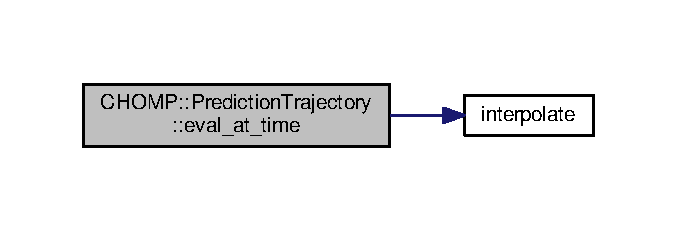
\includegraphics[width=325pt]{struct_c_h_o_m_p_1_1_prediction_trajectory_a3e50b3be07e9531449128eae47c60442_cgraph}
\end{center}
\end{figure}




Here is the caller graph for this function\+:
\nopagebreak
\begin{figure}[H]
\begin{center}
\leavevmode
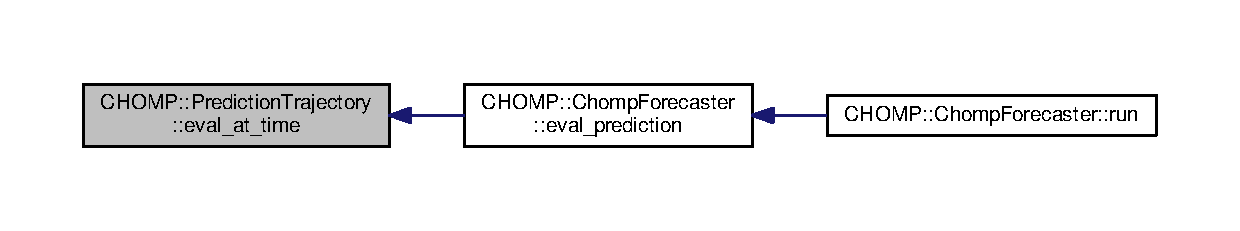
\includegraphics[width=350pt]{struct_c_h_o_m_p_1_1_prediction_trajectory_a3e50b3be07e9531449128eae47c60442_icgraph}
\end{center}
\end{figure}




\subsection{Member Data Documentation}
\index{C\+H\+O\+M\+P\+::\+Prediction\+Trajectory@{C\+H\+O\+M\+P\+::\+Prediction\+Trajectory}!pred\+\_\+path@{pred\+\_\+path}}
\index{pred\+\_\+path@{pred\+\_\+path}!C\+H\+O\+M\+P\+::\+Prediction\+Trajectory@{C\+H\+O\+M\+P\+::\+Prediction\+Trajectory}}
\subsubsection[{\texorpdfstring{pred\+\_\+path}{pred_path}}]{\setlength{\rightskip}{0pt plus 5cm}Matrix\+Xd C\+H\+O\+M\+P\+::\+Prediction\+Trajectory\+::pred\+\_\+path}\hypertarget{struct_c_h_o_m_p_1_1_prediction_trajectory_af07e1c23267f79f9e7ec029bcbb246b8}{}\label{struct_c_h_o_m_p_1_1_prediction_trajectory_af07e1c23267f79f9e7ec029bcbb246b8}


Definition at line 31 of file chomp\+\_\+predict.\+h.

\index{C\+H\+O\+M\+P\+::\+Prediction\+Trajectory@{C\+H\+O\+M\+P\+::\+Prediction\+Trajectory}!time\+\_\+seq@{time\+\_\+seq}}
\index{time\+\_\+seq@{time\+\_\+seq}!C\+H\+O\+M\+P\+::\+Prediction\+Trajectory@{C\+H\+O\+M\+P\+::\+Prediction\+Trajectory}}
\subsubsection[{\texorpdfstring{time\+\_\+seq}{time_seq}}]{\setlength{\rightskip}{0pt plus 5cm}Vector\+Xd C\+H\+O\+M\+P\+::\+Prediction\+Trajectory\+::time\+\_\+seq}\hypertarget{struct_c_h_o_m_p_1_1_prediction_trajectory_ae8b2997764b253ed927a7f24cea9a9fe}{}\label{struct_c_h_o_m_p_1_1_prediction_trajectory_ae8b2997764b253ed927a7f24cea9a9fe}


Definition at line 30 of file chomp\+\_\+predict.\+h.



The documentation for this struct was generated from the following file\+:\begin{DoxyCompactItemize}
\item 
include/chomp\+\_\+predict/\hyperlink{chomp__predict_8h}{chomp\+\_\+predict.\+h}\end{DoxyCompactItemize}

\hypertarget{struct_c_h_o_m_p_1_1_predict_param}{}\section{C\+H\+O\+MP\+:\+:Predict\+Param Struct Reference}
\label{struct_c_h_o_m_p_1_1_predict_param}\index{C\+H\+O\+M\+P\+::\+Predict\+Param@{C\+H\+O\+M\+P\+::\+Predict\+Param}}


{\ttfamily \#include $<$chomp\+\_\+predict.\+h$>$}

\subsection*{Public Member Functions}
\begin{DoxyCompactItemize}
\item 
double \hyperlink{struct_c_h_o_m_p_1_1_predict_param_ade19c94318f817105bf8b98725edb25f}{observation\+\_\+callback\+\_\+duration} ()
\end{DoxyCompactItemize}
\subsection*{Public Attributes}
\begin{DoxyCompactItemize}
\item 
int \hyperlink{struct_c_h_o_m_p_1_1_predict_param_a82c7cc8753b178ee7eee3ecb02960651}{No}
\item 
int \hyperlink{struct_c_h_o_m_p_1_1_predict_param_ab35ec9cff6cca550b5ba0b02a9b7b76c}{Np\+\_\+max}
\item 
int \hyperlink{struct_c_h_o_m_p_1_1_predict_param_a2f5cf53c69ea584acd95944b4fdd037f}{Np\+\_\+min}
\item 
double \hyperlink{struct_c_h_o_m_p_1_1_predict_param_ac11faa559b419145302aea082ded610e}{observation\+\_\+horizon}
\item 
double \hyperlink{struct_c_h_o_m_p_1_1_predict_param_a89a58ef3d9c88c23132ab5e7c64b9659}{prediction\+\_\+horizon}
\item 
double \hyperlink{struct_c_h_o_m_p_1_1_predict_param_a481fd775f165023e38e540757e0712ca}{trigger\+\_\+tol\+\_\+accum\+\_\+error}
\end{DoxyCompactItemize}


\subsection{Detailed Description}


Definition at line 13 of file chomp\+\_\+predict.\+h.



\subsection{Member Function Documentation}
\index{C\+H\+O\+M\+P\+::\+Predict\+Param@{C\+H\+O\+M\+P\+::\+Predict\+Param}!observation\+\_\+callback\+\_\+duration@{observation\+\_\+callback\+\_\+duration}}
\index{observation\+\_\+callback\+\_\+duration@{observation\+\_\+callback\+\_\+duration}!C\+H\+O\+M\+P\+::\+Predict\+Param@{C\+H\+O\+M\+P\+::\+Predict\+Param}}
\subsubsection[{\texorpdfstring{observation\+\_\+callback\+\_\+duration()}{observation_callback_duration()}}]{\setlength{\rightskip}{0pt plus 5cm}double C\+H\+O\+M\+P\+::\+Predict\+Param\+::observation\+\_\+callback\+\_\+duration (
\begin{DoxyParamCaption}
{}
\end{DoxyParamCaption}
)\hspace{0.3cm}{\ttfamily [inline]}}\hypertarget{struct_c_h_o_m_p_1_1_predict_param_ade19c94318f817105bf8b98725edb25f}{}\label{struct_c_h_o_m_p_1_1_predict_param_ade19c94318f817105bf8b98725edb25f}


Definition at line 20 of file chomp\+\_\+predict.\+h.



Here is the caller graph for this function\+:
\nopagebreak
\begin{figure}[H]
\begin{center}
\leavevmode
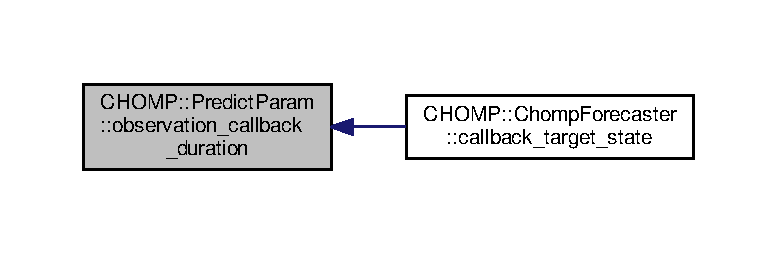
\includegraphics[width=350pt]{struct_c_h_o_m_p_1_1_predict_param_ade19c94318f817105bf8b98725edb25f_icgraph}
\end{center}
\end{figure}




\subsection{Member Data Documentation}
\index{C\+H\+O\+M\+P\+::\+Predict\+Param@{C\+H\+O\+M\+P\+::\+Predict\+Param}!No@{No}}
\index{No@{No}!C\+H\+O\+M\+P\+::\+Predict\+Param@{C\+H\+O\+M\+P\+::\+Predict\+Param}}
\subsubsection[{\texorpdfstring{No}{No}}]{\setlength{\rightskip}{0pt plus 5cm}int C\+H\+O\+M\+P\+::\+Predict\+Param\+::\+No}\hypertarget{struct_c_h_o_m_p_1_1_predict_param_a82c7cc8753b178ee7eee3ecb02960651}{}\label{struct_c_h_o_m_p_1_1_predict_param_a82c7cc8753b178ee7eee3ecb02960651}


Definition at line 14 of file chomp\+\_\+predict.\+h.

\index{C\+H\+O\+M\+P\+::\+Predict\+Param@{C\+H\+O\+M\+P\+::\+Predict\+Param}!Np\+\_\+max@{Np\+\_\+max}}
\index{Np\+\_\+max@{Np\+\_\+max}!C\+H\+O\+M\+P\+::\+Predict\+Param@{C\+H\+O\+M\+P\+::\+Predict\+Param}}
\subsubsection[{\texorpdfstring{Np\+\_\+max}{Np_max}}]{\setlength{\rightskip}{0pt plus 5cm}int C\+H\+O\+M\+P\+::\+Predict\+Param\+::\+Np\+\_\+max}\hypertarget{struct_c_h_o_m_p_1_1_predict_param_ab35ec9cff6cca550b5ba0b02a9b7b76c}{}\label{struct_c_h_o_m_p_1_1_predict_param_ab35ec9cff6cca550b5ba0b02a9b7b76c}


Definition at line 15 of file chomp\+\_\+predict.\+h.

\index{C\+H\+O\+M\+P\+::\+Predict\+Param@{C\+H\+O\+M\+P\+::\+Predict\+Param}!Np\+\_\+min@{Np\+\_\+min}}
\index{Np\+\_\+min@{Np\+\_\+min}!C\+H\+O\+M\+P\+::\+Predict\+Param@{C\+H\+O\+M\+P\+::\+Predict\+Param}}
\subsubsection[{\texorpdfstring{Np\+\_\+min}{Np_min}}]{\setlength{\rightskip}{0pt plus 5cm}int C\+H\+O\+M\+P\+::\+Predict\+Param\+::\+Np\+\_\+min}\hypertarget{struct_c_h_o_m_p_1_1_predict_param_a2f5cf53c69ea584acd95944b4fdd037f}{}\label{struct_c_h_o_m_p_1_1_predict_param_a2f5cf53c69ea584acd95944b4fdd037f}


Definition at line 16 of file chomp\+\_\+predict.\+h.

\index{C\+H\+O\+M\+P\+::\+Predict\+Param@{C\+H\+O\+M\+P\+::\+Predict\+Param}!observation\+\_\+horizon@{observation\+\_\+horizon}}
\index{observation\+\_\+horizon@{observation\+\_\+horizon}!C\+H\+O\+M\+P\+::\+Predict\+Param@{C\+H\+O\+M\+P\+::\+Predict\+Param}}
\subsubsection[{\texorpdfstring{observation\+\_\+horizon}{observation_horizon}}]{\setlength{\rightskip}{0pt plus 5cm}double C\+H\+O\+M\+P\+::\+Predict\+Param\+::observation\+\_\+horizon}\hypertarget{struct_c_h_o_m_p_1_1_predict_param_ac11faa559b419145302aea082ded610e}{}\label{struct_c_h_o_m_p_1_1_predict_param_ac11faa559b419145302aea082ded610e}


Definition at line 17 of file chomp\+\_\+predict.\+h.

\index{C\+H\+O\+M\+P\+::\+Predict\+Param@{C\+H\+O\+M\+P\+::\+Predict\+Param}!prediction\+\_\+horizon@{prediction\+\_\+horizon}}
\index{prediction\+\_\+horizon@{prediction\+\_\+horizon}!C\+H\+O\+M\+P\+::\+Predict\+Param@{C\+H\+O\+M\+P\+::\+Predict\+Param}}
\subsubsection[{\texorpdfstring{prediction\+\_\+horizon}{prediction_horizon}}]{\setlength{\rightskip}{0pt plus 5cm}double C\+H\+O\+M\+P\+::\+Predict\+Param\+::prediction\+\_\+horizon}\hypertarget{struct_c_h_o_m_p_1_1_predict_param_a89a58ef3d9c88c23132ab5e7c64b9659}{}\label{struct_c_h_o_m_p_1_1_predict_param_a89a58ef3d9c88c23132ab5e7c64b9659}


Definition at line 18 of file chomp\+\_\+predict.\+h.

\index{C\+H\+O\+M\+P\+::\+Predict\+Param@{C\+H\+O\+M\+P\+::\+Predict\+Param}!trigger\+\_\+tol\+\_\+accum\+\_\+error@{trigger\+\_\+tol\+\_\+accum\+\_\+error}}
\index{trigger\+\_\+tol\+\_\+accum\+\_\+error@{trigger\+\_\+tol\+\_\+accum\+\_\+error}!C\+H\+O\+M\+P\+::\+Predict\+Param@{C\+H\+O\+M\+P\+::\+Predict\+Param}}
\subsubsection[{\texorpdfstring{trigger\+\_\+tol\+\_\+accum\+\_\+error}{trigger_tol_accum_error}}]{\setlength{\rightskip}{0pt plus 5cm}double C\+H\+O\+M\+P\+::\+Predict\+Param\+::trigger\+\_\+tol\+\_\+accum\+\_\+error}\hypertarget{struct_c_h_o_m_p_1_1_predict_param_a481fd775f165023e38e540757e0712ca}{}\label{struct_c_h_o_m_p_1_1_predict_param_a481fd775f165023e38e540757e0712ca}


Definition at line 19 of file chomp\+\_\+predict.\+h.



The documentation for this struct was generated from the following file\+:\begin{DoxyCompactItemize}
\item 
include/chomp\+\_\+predict/\hyperlink{chomp__predict_8h}{chomp\+\_\+predict.\+h}\end{DoxyCompactItemize}

\hypertarget{class_c_h_o_m_p_1_1_solver}{}\section{C\+H\+O\+MP\+:\+:Solver Class Reference}
\label{class_c_h_o_m_p_1_1_solver}\index{C\+H\+O\+M\+P\+::\+Solver@{C\+H\+O\+M\+P\+::\+Solver}}


{\ttfamily \#include $<$chomp\+\_\+subroutine.\+h$>$}

\subsection*{Public Member Functions}
\begin{DoxyCompactItemize}
\item 
\hyperlink{class_c_h_o_m_p_1_1_solver_a9dfe7ae9ce617e8a6398be34284c907a}{Solver} ()
\item 
void \hyperlink{class_c_h_o_m_p_1_1_solver_ac27fc3241bd65b38d832d9838ab64641}{set\+\_\+problem} (Matrix\+Xd A, Vector\+Xd b, Dynamic\+E\+D\+T\+Octomap $\ast$, \hyperlink{struct_c_h_o_m_p_1_1_cost_param}{Cost\+Param})
\item 
void \hyperlink{class_c_h_o_m_p_1_1_solver_a8a87ee9ad9182fd2e4e913cb24051a6c}{set\+\_\+problem} (Matrix\+Xd A, Vector\+Xd b, voxblox\+::\+Esdf\+Server $\ast$, \hyperlink{struct_c_h_o_m_p_1_1_cost_param}{Cost\+Param})
\item 
\hyperlink{struct_c_h_o_m_p_1_1_optim_result}{Optim\+Result} \hyperlink{class_c_h_o_m_p_1_1_solver_a677d1b1adb6a2c4f490d47f5fcabfe0d}{solve} (Vector\+Xd x0, \hyperlink{struct_c_h_o_m_p_1_1_optim_param}{Optim\+Param} optimization\+\_\+param)
\end{DoxyCompactItemize}


\subsection{Detailed Description}


Definition at line 50 of file chomp\+\_\+subroutine.\+h.



\subsection{Constructor \& Destructor Documentation}
\index{C\+H\+O\+M\+P\+::\+Solver@{C\+H\+O\+M\+P\+::\+Solver}!Solver@{Solver}}
\index{Solver@{Solver}!C\+H\+O\+M\+P\+::\+Solver@{C\+H\+O\+M\+P\+::\+Solver}}
\subsubsection[{\texorpdfstring{Solver()}{Solver()}}]{\setlength{\rightskip}{0pt plus 5cm}Solver\+::\+Solver (
\begin{DoxyParamCaption}
{}
\end{DoxyParamCaption}
)}\hypertarget{class_c_h_o_m_p_1_1_solver_a9dfe7ae9ce617e8a6398be34284c907a}{}\label{class_c_h_o_m_p_1_1_solver_a9dfe7ae9ce617e8a6398be34284c907a}


Definition at line 5 of file chomp\+\_\+subroutine.\+cpp.



\subsection{Member Function Documentation}
\index{C\+H\+O\+M\+P\+::\+Solver@{C\+H\+O\+M\+P\+::\+Solver}!set\+\_\+problem@{set\+\_\+problem}}
\index{set\+\_\+problem@{set\+\_\+problem}!C\+H\+O\+M\+P\+::\+Solver@{C\+H\+O\+M\+P\+::\+Solver}}
\subsubsection[{\texorpdfstring{set\+\_\+problem(\+Matrix\+Xd A, Vector\+Xd b, Dynamic\+E\+D\+T\+Octomap $\ast$, Cost\+Param)}{set_problem(MatrixXd A, VectorXd b, DynamicEDTOctomap *, CostParam)}}]{\setlength{\rightskip}{0pt plus 5cm}void Solver\+::set\+\_\+problem (
\begin{DoxyParamCaption}
\item[{Matrix\+Xd}]{A, }
\item[{Vector\+Xd}]{b, }
\item[{Dynamic\+E\+D\+T\+Octomap $\ast$}]{edf, }
\item[{{\bf Cost\+Param}}]{cost\+\_\+param}
\end{DoxyParamCaption}
)}\hypertarget{class_c_h_o_m_p_1_1_solver_ac27fc3241bd65b38d832d9838ab64641}{}\label{class_c_h_o_m_p_1_1_solver_ac27fc3241bd65b38d832d9838ab64641}


Definition at line 7 of file chomp\+\_\+subroutine.\+cpp.



Here is the caller graph for this function\+:
\nopagebreak
\begin{figure}[H]
\begin{center}
\leavevmode
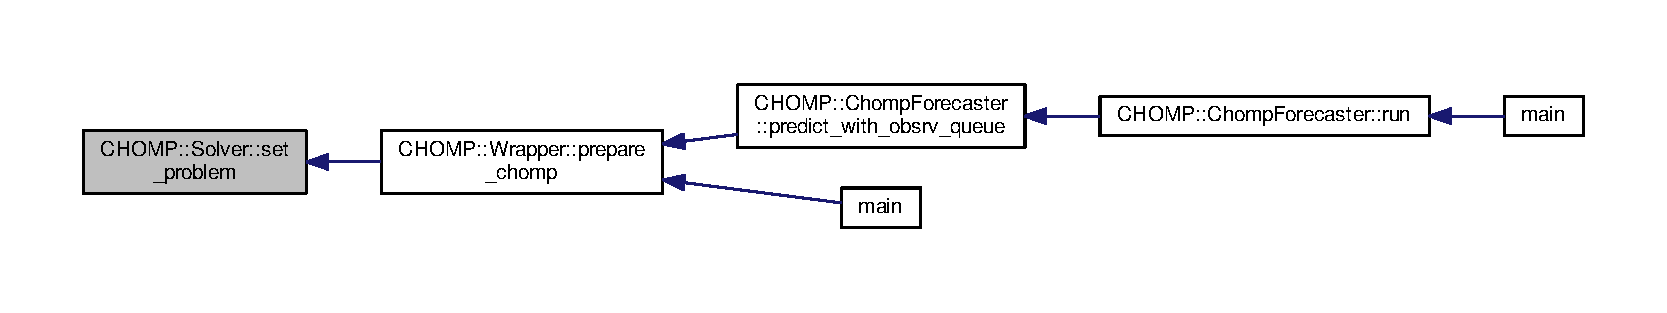
\includegraphics[width=350pt]{class_c_h_o_m_p_1_1_solver_ac27fc3241bd65b38d832d9838ab64641_icgraph}
\end{center}
\end{figure}


\index{C\+H\+O\+M\+P\+::\+Solver@{C\+H\+O\+M\+P\+::\+Solver}!set\+\_\+problem@{set\+\_\+problem}}
\index{set\+\_\+problem@{set\+\_\+problem}!C\+H\+O\+M\+P\+::\+Solver@{C\+H\+O\+M\+P\+::\+Solver}}
\subsubsection[{\texorpdfstring{set\+\_\+problem(\+Matrix\+Xd A, Vector\+Xd b, voxblox\+::\+Esdf\+Server $\ast$, Cost\+Param)}{set_problem(MatrixXd A, VectorXd b, voxblox::EsdfServer *, CostParam)}}]{\setlength{\rightskip}{0pt plus 5cm}void Solver\+::set\+\_\+problem (
\begin{DoxyParamCaption}
\item[{Matrix\+Xd}]{A, }
\item[{Vector\+Xd}]{b, }
\item[{voxblox\+::\+Esdf\+Server $\ast$}]{esdf\+\_\+ptr, }
\item[{{\bf Cost\+Param}}]{cost\+\_\+param}
\end{DoxyParamCaption}
)}\hypertarget{class_c_h_o_m_p_1_1_solver_a8a87ee9ad9182fd2e4e913cb24051a6c}{}\label{class_c_h_o_m_p_1_1_solver_a8a87ee9ad9182fd2e4e913cb24051a6c}


Definition at line 20 of file chomp\+\_\+subroutine.\+cpp.

\index{C\+H\+O\+M\+P\+::\+Solver@{C\+H\+O\+M\+P\+::\+Solver}!solve@{solve}}
\index{solve@{solve}!C\+H\+O\+M\+P\+::\+Solver@{C\+H\+O\+M\+P\+::\+Solver}}
\subsubsection[{\texorpdfstring{solve(\+Vector\+Xd x0, Optim\+Param optimization\+\_\+param)}{solve(VectorXd x0, OptimParam optimization_param)}}]{\setlength{\rightskip}{0pt plus 5cm}{\bf Optim\+Result} Solver\+::solve (
\begin{DoxyParamCaption}
\item[{Vector\+Xd}]{x0, }
\item[{{\bf Optim\+Param}}]{optimization\+\_\+param}
\end{DoxyParamCaption}
)}\hypertarget{class_c_h_o_m_p_1_1_solver_a677d1b1adb6a2c4f490d47f5fcabfe0d}{}\label{class_c_h_o_m_p_1_1_solver_a677d1b1adb6a2c4f490d47f5fcabfe0d}


Definition at line 36 of file chomp\+\_\+subroutine.\+cpp.



Here is the caller graph for this function\+:
\nopagebreak
\begin{figure}[H]
\begin{center}
\leavevmode
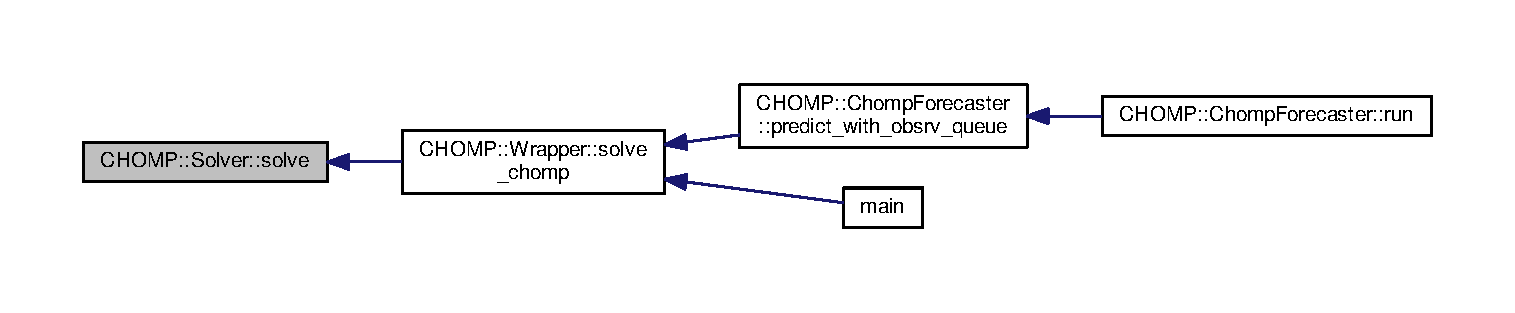
\includegraphics[width=350pt]{class_c_h_o_m_p_1_1_solver_a677d1b1adb6a2c4f490d47f5fcabfe0d_icgraph}
\end{center}
\end{figure}




The documentation for this class was generated from the following files\+:\begin{DoxyCompactItemize}
\item 
include/chomp\+\_\+predict/\hyperlink{chomp__subroutine_8h}{chomp\+\_\+subroutine.\+h}\item 
src/\hyperlink{chomp__subroutine_8cpp}{chomp\+\_\+subroutine.\+cpp}\end{DoxyCompactItemize}

\hypertarget{class_c_h_o_m_p_1_1_wrapper}{}\section{C\+H\+O\+MP\+:\+:Wrapper Class Reference}
\label{class_c_h_o_m_p_1_1_wrapper}\index{C\+H\+O\+M\+P\+::\+Wrapper@{C\+H\+O\+M\+P\+::\+Wrapper}}


{\ttfamily \#include $<$chomp\+\_\+ros\+\_\+wrapper.\+h$>$}



Collaboration diagram for C\+H\+O\+MP\+:\+:Wrapper\+:
\nopagebreak
\begin{figure}[H]
\begin{center}
\leavevmode
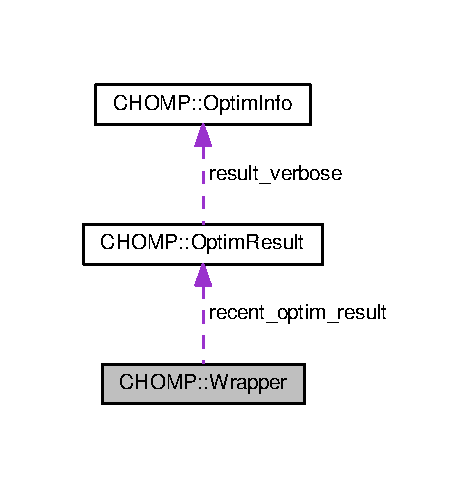
\includegraphics[width=227pt]{class_c_h_o_m_p_1_1_wrapper__coll__graph}
\end{center}
\end{figure}
\subsection*{Public Member Functions}
\begin{DoxyCompactItemize}
\item 
\hyperlink{class_c_h_o_m_p_1_1_wrapper_a6eb8cdd0f948a2a5e698c66e890e8e0e}{Wrapper} (const ros\+::\+Node\+Handle \&)
\item 
void \hyperlink{class_c_h_o_m_p_1_1_wrapper_a6ddf801481c8cb4d567ea7cb073a819b}{load\+\_\+markers\+\_\+prior\+\_\+pnts} (nav\+\_\+msgs\+::\+Path prior\+\_\+path, geometry\+\_\+msgs\+::\+Point goal)
\item 
void \hyperlink{class_c_h_o_m_p_1_1_wrapper_a84f5c4690636e65aca526e6e5b8abcf4}{publish\+\_\+routine} ()
\item 
void \hyperlink{class_c_h_o_m_p_1_1_wrapper_a095c001d0a11f0fa4229e38f602e5931}{load\+\_\+map} (octomap\+::\+Oc\+Tree $\ast$octree\+\_\+ptr)
\item 
void \hyperlink{class_c_h_o_m_p_1_1_wrapper_a93b14d4809f5bf3170473fc10a93a755}{load\+\_\+map} (string file\+\_\+name)
\item 
void \hyperlink{class_c_h_o_m_p_1_1_wrapper_ab51d0a655ed4b03ca3225c0af737f2dc}{build\+\_\+matrix} (Matrix\+Xd \&A, Vector\+Xd \&b, nav\+\_\+msgs\+::\+Path prior\+\_\+points, geometry\+\_\+msgs\+::\+Point goal, \hyperlink{struct_c_h_o_m_p_1_1_optim_param}{Optim\+Param} $\ast$param=N\+U\+LL)
\begin{DoxyCompactList}\small\item\em build prior term from prior points (start\+\_\+pnt) of length No+1(No observations and one final point) to make 1/2x\textquotesingle{}Mx+hx \end{DoxyCompactList}\item 
Vector\+Xd \hyperlink{class_c_h_o_m_p_1_1_wrapper_a138ac0d5088055c3698d93bbf9432126}{prepare\+\_\+chomp} (Matrix\+Xd A, Vector\+Xd b, nav\+\_\+msgs\+::\+Path prior\+\_\+path, geometry\+\_\+msgs\+::\+Point goal, \hyperlink{struct_c_h_o_m_p_1_1_optim_param}{Optim\+Param} $\ast$param=N\+U\+LL)
\item 
bool \hyperlink{class_c_h_o_m_p_1_1_wrapper_ac8fa793a31b7872feccc711c55c1da20}{solve\+\_\+chomp} (Vector\+Xd x0)
\item 
Matrix\+Xd \hyperlink{class_c_h_o_m_p_1_1_wrapper_ae94071b38bb2cd68d4a281c9f93e9587}{get\+\_\+current\+\_\+prediction\+\_\+path} ()
\item 
\hyperlink{struct_c_h_o_m_p_1_1_optim_param}{Optim\+Param} \hyperlink{class_c_h_o_m_p_1_1_wrapper_ac31da0a2c980d5b64541852f01deebbf}{get\+\_\+default\+\_\+optim\+\_\+param} ()
\item 
double \hyperlink{class_c_h_o_m_p_1_1_wrapper_aa4af50daa2bae57af10cdd344571c5af}{get\+\_\+ground\+\_\+height} ()
\end{DoxyCompactItemize}
\subsection*{Public Attributes}
\begin{DoxyCompactItemize}
\item 
\hyperlink{struct_c_h_o_m_p_1_1_optim_result}{Optim\+Result} \hyperlink{class_c_h_o_m_p_1_1_wrapper_a5b349bddf6965d721705e451601687a7}{recent\+\_\+optim\+\_\+result}
\item 
int \hyperlink{class_c_h_o_m_p_1_1_wrapper_a8e7d4dd9f8678e2752ef05e55a36ffe1}{map\+\_\+type}
\end{DoxyCompactItemize}


\subsection{Detailed Description}


Definition at line 12 of file chomp\+\_\+ros\+\_\+wrapper.\+h.



\subsection{Constructor \& Destructor Documentation}
\index{C\+H\+O\+M\+P\+::\+Wrapper@{C\+H\+O\+M\+P\+::\+Wrapper}!Wrapper@{Wrapper}}
\index{Wrapper@{Wrapper}!C\+H\+O\+M\+P\+::\+Wrapper@{C\+H\+O\+M\+P\+::\+Wrapper}}
\subsubsection[{\texorpdfstring{Wrapper(const ros\+::\+Node\+Handle \&)}{Wrapper(const ros::NodeHandle &)}}]{\setlength{\rightskip}{0pt plus 5cm}Wrapper\+::\+Wrapper (
\begin{DoxyParamCaption}
\item[{const ros\+::\+Node\+Handle \&}]{nh\+\_\+global}
\end{DoxyParamCaption}
)}\hypertarget{class_c_h_o_m_p_1_1_wrapper_a6eb8cdd0f948a2a5e698c66e890e8e0e}{}\label{class_c_h_o_m_p_1_1_wrapper_a6eb8cdd0f948a2a5e698c66e890e8e0e}


Definition at line 5 of file chomp\+\_\+ros\+\_\+wrapper.\+cpp.



\subsection{Member Function Documentation}
\index{C\+H\+O\+M\+P\+::\+Wrapper@{C\+H\+O\+M\+P\+::\+Wrapper}!build\+\_\+matrix@{build\+\_\+matrix}}
\index{build\+\_\+matrix@{build\+\_\+matrix}!C\+H\+O\+M\+P\+::\+Wrapper@{C\+H\+O\+M\+P\+::\+Wrapper}}
\subsubsection[{\texorpdfstring{build\+\_\+matrix(\+Matrix\+Xd \&\+A, Vector\+Xd \&b, nav\+\_\+msgs\+::\+Path prior\+\_\+points, geometry\+\_\+msgs\+::\+Point goal, Optim\+Param $\ast$param=\+N\+U\+L\+L)}{build_matrix(MatrixXd &A, VectorXd &b, nav_msgs::Path prior_points, geometry_msgs::Point goal, OptimParam *param=NULL)}}]{\setlength{\rightskip}{0pt plus 5cm}void Wrapper\+::build\+\_\+matrix (
\begin{DoxyParamCaption}
\item[{Matrix\+Xd \&}]{M, }
\item[{Vector\+Xd \&}]{h, }
\item[{nav\+\_\+msgs\+::\+Path}]{prior\+\_\+points, }
\item[{geometry\+\_\+msgs\+::\+Point}]{goal, }
\item[{{\bf Optim\+Param} $\ast$}]{param = {\ttfamily NULL}}
\end{DoxyParamCaption}
)}\hypertarget{class_c_h_o_m_p_1_1_wrapper_ab51d0a655ed4b03ca3225c0af737f2dc}{}\label{class_c_h_o_m_p_1_1_wrapper_ab51d0a655ed4b03ca3225c0af737f2dc}


build prior term from prior points (start\+\_\+pnt) of length No+1(No observations and one final point) to make 1/2x\textquotesingle{}Mx+hx 


\begin{DoxyParams}{Parameters}
{\em M} & insert matrix to M \\
\hline
{\em h} & insert matrix to h \\
\hline
{\em prior\+\_\+points} & points of length No$<$=N \\
\hline
{\em gamma} & weight factor for prior points \\
\hline
{\em goal} & goal point \\
\hline
{\em N} & total time index \\
\hline
\end{DoxyParams}


Definition at line 112 of file chomp\+\_\+ros\+\_\+wrapper.\+cpp.



Here is the caller graph for this function\+:
\nopagebreak
\begin{figure}[H]
\begin{center}
\leavevmode
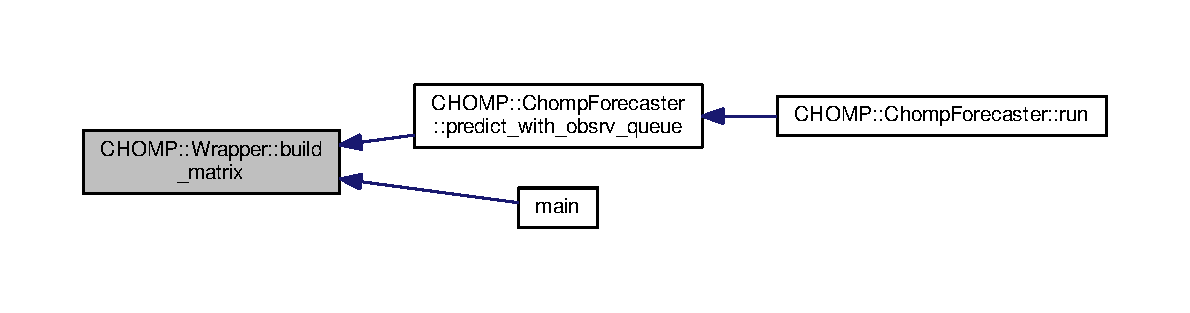
\includegraphics[width=350pt]{class_c_h_o_m_p_1_1_wrapper_ab51d0a655ed4b03ca3225c0af737f2dc_icgraph}
\end{center}
\end{figure}


\index{C\+H\+O\+M\+P\+::\+Wrapper@{C\+H\+O\+M\+P\+::\+Wrapper}!get\+\_\+current\+\_\+prediction\+\_\+path@{get\+\_\+current\+\_\+prediction\+\_\+path}}
\index{get\+\_\+current\+\_\+prediction\+\_\+path@{get\+\_\+current\+\_\+prediction\+\_\+path}!C\+H\+O\+M\+P\+::\+Wrapper@{C\+H\+O\+M\+P\+::\+Wrapper}}
\subsubsection[{\texorpdfstring{get\+\_\+current\+\_\+prediction\+\_\+path()}{get_current_prediction_path()}}]{\setlength{\rightskip}{0pt plus 5cm}Matrix\+Xd Wrapper\+::get\+\_\+current\+\_\+prediction\+\_\+path (
\begin{DoxyParamCaption}
{}
\end{DoxyParamCaption}
)}\hypertarget{class_c_h_o_m_p_1_1_wrapper_ae94071b38bb2cd68d4a281c9f93e9587}{}\label{class_c_h_o_m_p_1_1_wrapper_ae94071b38bb2cd68d4a281c9f93e9587}


Definition at line 298 of file chomp\+\_\+ros\+\_\+wrapper.\+cpp.



Here is the caller graph for this function\+:
\nopagebreak
\begin{figure}[H]
\begin{center}
\leavevmode
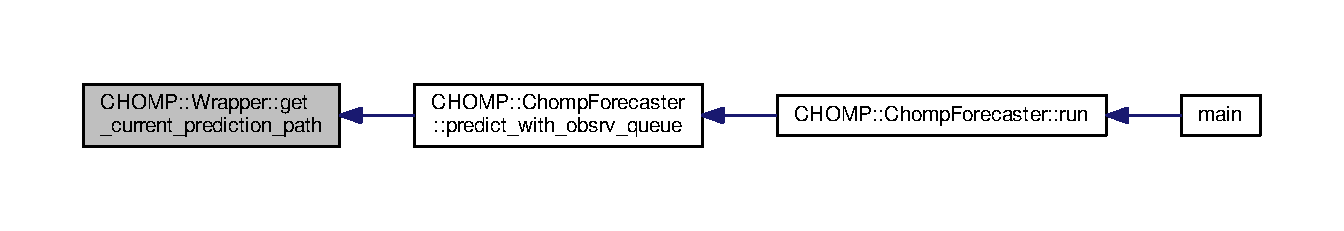
\includegraphics[width=350pt]{class_c_h_o_m_p_1_1_wrapper_ae94071b38bb2cd68d4a281c9f93e9587_icgraph}
\end{center}
\end{figure}


\index{C\+H\+O\+M\+P\+::\+Wrapper@{C\+H\+O\+M\+P\+::\+Wrapper}!get\+\_\+default\+\_\+optim\+\_\+param@{get\+\_\+default\+\_\+optim\+\_\+param}}
\index{get\+\_\+default\+\_\+optim\+\_\+param@{get\+\_\+default\+\_\+optim\+\_\+param}!C\+H\+O\+M\+P\+::\+Wrapper@{C\+H\+O\+M\+P\+::\+Wrapper}}
\subsubsection[{\texorpdfstring{get\+\_\+default\+\_\+optim\+\_\+param()}{get_default_optim_param()}}]{\setlength{\rightskip}{0pt plus 5cm}{\bf Optim\+Param} Wrapper\+::get\+\_\+default\+\_\+optim\+\_\+param (
\begin{DoxyParamCaption}
{}
\end{DoxyParamCaption}
)}\hypertarget{class_c_h_o_m_p_1_1_wrapper_ac31da0a2c980d5b64541852f01deebbf}{}\label{class_c_h_o_m_p_1_1_wrapper_ac31da0a2c980d5b64541852f01deebbf}


Definition at line 319 of file chomp\+\_\+ros\+\_\+wrapper.\+cpp.



Here is the caller graph for this function\+:
\nopagebreak
\begin{figure}[H]
\begin{center}
\leavevmode
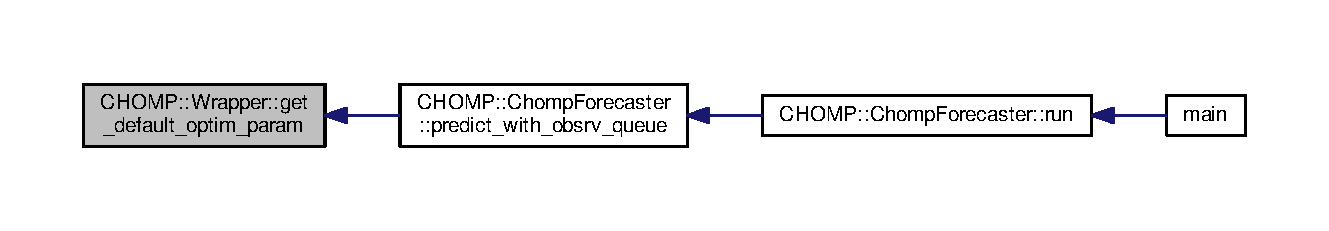
\includegraphics[width=350pt]{class_c_h_o_m_p_1_1_wrapper_ac31da0a2c980d5b64541852f01deebbf_icgraph}
\end{center}
\end{figure}


\index{C\+H\+O\+M\+P\+::\+Wrapper@{C\+H\+O\+M\+P\+::\+Wrapper}!get\+\_\+ground\+\_\+height@{get\+\_\+ground\+\_\+height}}
\index{get\+\_\+ground\+\_\+height@{get\+\_\+ground\+\_\+height}!C\+H\+O\+M\+P\+::\+Wrapper@{C\+H\+O\+M\+P\+::\+Wrapper}}
\subsubsection[{\texorpdfstring{get\+\_\+ground\+\_\+height()}{get_ground_height()}}]{\setlength{\rightskip}{0pt plus 5cm}double C\+H\+O\+M\+P\+::\+Wrapper\+::get\+\_\+ground\+\_\+height (
\begin{DoxyParamCaption}
{}
\end{DoxyParamCaption}
)\hspace{0.3cm}{\ttfamily [inline]}}\hypertarget{class_c_h_o_m_p_1_1_wrapper_aa4af50daa2bae57af10cdd344571c5af}{}\label{class_c_h_o_m_p_1_1_wrapper_aa4af50daa2bae57af10cdd344571c5af}


Definition at line 67 of file chomp\+\_\+ros\+\_\+wrapper.\+h.



Here is the caller graph for this function\+:
\nopagebreak
\begin{figure}[H]
\begin{center}
\leavevmode
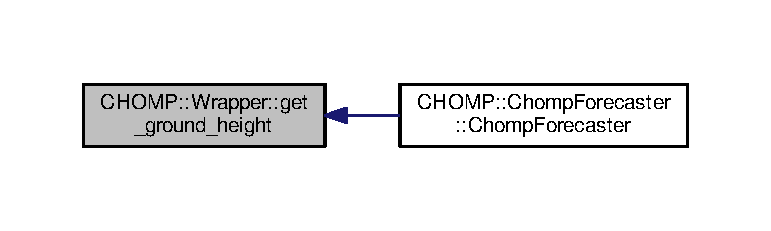
\includegraphics[width=350pt]{class_c_h_o_m_p_1_1_wrapper_aa4af50daa2bae57af10cdd344571c5af_icgraph}
\end{center}
\end{figure}


\index{C\+H\+O\+M\+P\+::\+Wrapper@{C\+H\+O\+M\+P\+::\+Wrapper}!load\+\_\+map@{load\+\_\+map}}
\index{load\+\_\+map@{load\+\_\+map}!C\+H\+O\+M\+P\+::\+Wrapper@{C\+H\+O\+M\+P\+::\+Wrapper}}
\subsubsection[{\texorpdfstring{load\+\_\+map(octomap\+::\+Oc\+Tree $\ast$octree\+\_\+ptr)}{load_map(octomap::OcTree *octree_ptr)}}]{\setlength{\rightskip}{0pt plus 5cm}void Wrapper\+::load\+\_\+map (
\begin{DoxyParamCaption}
\item[{octomap\+::\+Oc\+Tree $\ast$}]{octree\+\_\+ptr}
\end{DoxyParamCaption}
)}\hypertarget{class_c_h_o_m_p_1_1_wrapper_a095c001d0a11f0fa4229e38f602e5931}{}\label{class_c_h_o_m_p_1_1_wrapper_a095c001d0a11f0fa4229e38f602e5931}


Definition at line 71 of file chomp\+\_\+ros\+\_\+wrapper.\+cpp.



Here is the caller graph for this function\+:
\nopagebreak
\begin{figure}[H]
\begin{center}
\leavevmode
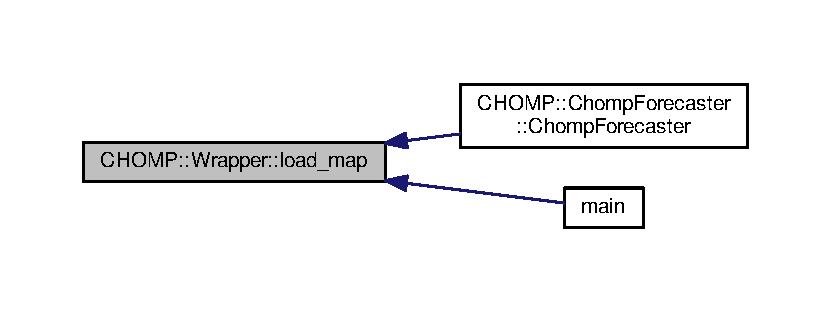
\includegraphics[width=350pt]{class_c_h_o_m_p_1_1_wrapper_a095c001d0a11f0fa4229e38f602e5931_icgraph}
\end{center}
\end{figure}


\index{C\+H\+O\+M\+P\+::\+Wrapper@{C\+H\+O\+M\+P\+::\+Wrapper}!load\+\_\+map@{load\+\_\+map}}
\index{load\+\_\+map@{load\+\_\+map}!C\+H\+O\+M\+P\+::\+Wrapper@{C\+H\+O\+M\+P\+::\+Wrapper}}
\subsubsection[{\texorpdfstring{load\+\_\+map(string file\+\_\+name)}{load_map(string file_name)}}]{\setlength{\rightskip}{0pt plus 5cm}void Wrapper\+::load\+\_\+map (
\begin{DoxyParamCaption}
\item[{string}]{file\+\_\+name}
\end{DoxyParamCaption}
)}\hypertarget{class_c_h_o_m_p_1_1_wrapper_a93b14d4809f5bf3170473fc10a93a755}{}\label{class_c_h_o_m_p_1_1_wrapper_a93b14d4809f5bf3170473fc10a93a755}


Definition at line 94 of file chomp\+\_\+ros\+\_\+wrapper.\+cpp.

\index{C\+H\+O\+M\+P\+::\+Wrapper@{C\+H\+O\+M\+P\+::\+Wrapper}!load\+\_\+markers\+\_\+prior\+\_\+pnts@{load\+\_\+markers\+\_\+prior\+\_\+pnts}}
\index{load\+\_\+markers\+\_\+prior\+\_\+pnts@{load\+\_\+markers\+\_\+prior\+\_\+pnts}!C\+H\+O\+M\+P\+::\+Wrapper@{C\+H\+O\+M\+P\+::\+Wrapper}}
\subsubsection[{\texorpdfstring{load\+\_\+markers\+\_\+prior\+\_\+pnts(nav\+\_\+msgs\+::\+Path prior\+\_\+path, geometry\+\_\+msgs\+::\+Point goal)}{load_markers_prior_pnts(nav_msgs::Path prior_path, geometry_msgs::Point goal)}}]{\setlength{\rightskip}{0pt plus 5cm}void Wrapper\+::load\+\_\+markers\+\_\+prior\+\_\+pnts (
\begin{DoxyParamCaption}
\item[{nav\+\_\+msgs\+::\+Path}]{prior\+\_\+path, }
\item[{geometry\+\_\+msgs\+::\+Point}]{goal}
\end{DoxyParamCaption}
)}\hypertarget{class_c_h_o_m_p_1_1_wrapper_a6ddf801481c8cb4d567ea7cb073a819b}{}\label{class_c_h_o_m_p_1_1_wrapper_a6ddf801481c8cb4d567ea7cb073a819b}


Definition at line 43 of file chomp\+\_\+ros\+\_\+wrapper.\+cpp.



Here is the caller graph for this function\+:
\nopagebreak
\begin{figure}[H]
\begin{center}
\leavevmode
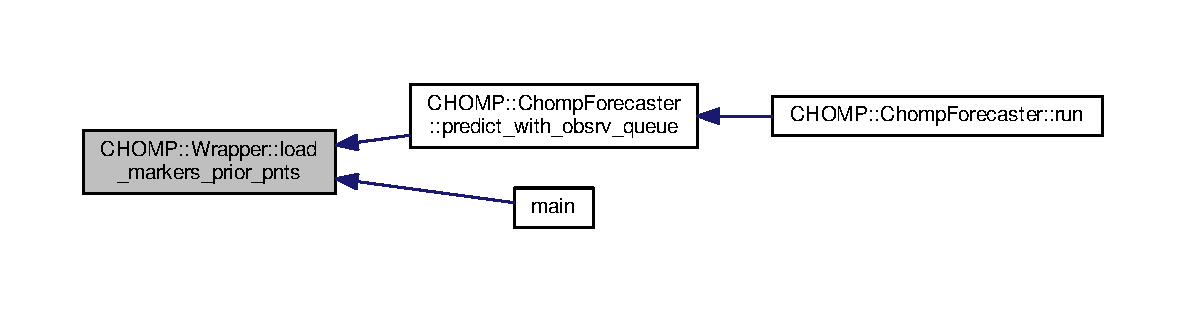
\includegraphics[width=350pt]{class_c_h_o_m_p_1_1_wrapper_a6ddf801481c8cb4d567ea7cb073a819b_icgraph}
\end{center}
\end{figure}


\index{C\+H\+O\+M\+P\+::\+Wrapper@{C\+H\+O\+M\+P\+::\+Wrapper}!prepare\+\_\+chomp@{prepare\+\_\+chomp}}
\index{prepare\+\_\+chomp@{prepare\+\_\+chomp}!C\+H\+O\+M\+P\+::\+Wrapper@{C\+H\+O\+M\+P\+::\+Wrapper}}
\subsubsection[{\texorpdfstring{prepare\+\_\+chomp(\+Matrix\+Xd A, Vector\+Xd b, nav\+\_\+msgs\+::\+Path prior\+\_\+path, geometry\+\_\+msgs\+::\+Point goal, Optim\+Param $\ast$param=\+N\+U\+L\+L)}{prepare_chomp(MatrixXd A, VectorXd b, nav_msgs::Path prior_path, geometry_msgs::Point goal, OptimParam *param=NULL)}}]{\setlength{\rightskip}{0pt plus 5cm}Vector\+Xd Wrapper\+::prepare\+\_\+chomp (
\begin{DoxyParamCaption}
\item[{Matrix\+Xd}]{A, }
\item[{Vector\+Xd}]{b, }
\item[{nav\+\_\+msgs\+::\+Path}]{prior\+\_\+path, }
\item[{geometry\+\_\+msgs\+::\+Point}]{goal, }
\item[{{\bf Optim\+Param} $\ast$}]{param = {\ttfamily NULL}}
\end{DoxyParamCaption}
)}\hypertarget{class_c_h_o_m_p_1_1_wrapper_a138ac0d5088055c3698d93bbf9432126}{}\label{class_c_h_o_m_p_1_1_wrapper_a138ac0d5088055c3698d93bbf9432126}


Definition at line 185 of file chomp\+\_\+ros\+\_\+wrapper.\+cpp.



Here is the call graph for this function\+:\nopagebreak
\begin{figure}[H]
\begin{center}
\leavevmode
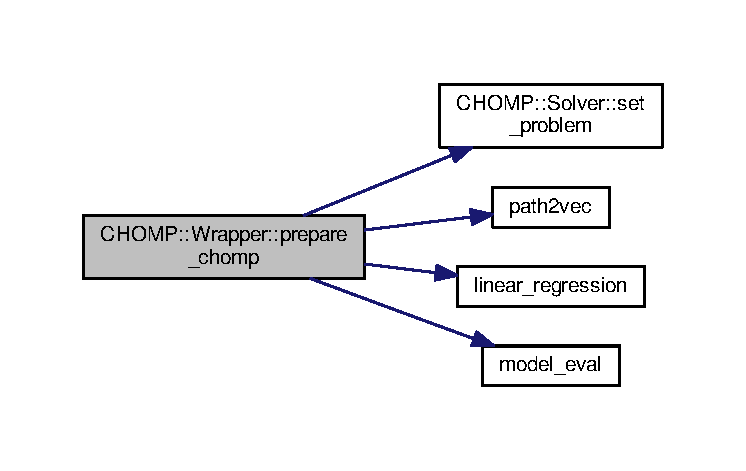
\includegraphics[width=350pt]{class_c_h_o_m_p_1_1_wrapper_a138ac0d5088055c3698d93bbf9432126_cgraph}
\end{center}
\end{figure}




Here is the caller graph for this function\+:
\nopagebreak
\begin{figure}[H]
\begin{center}
\leavevmode
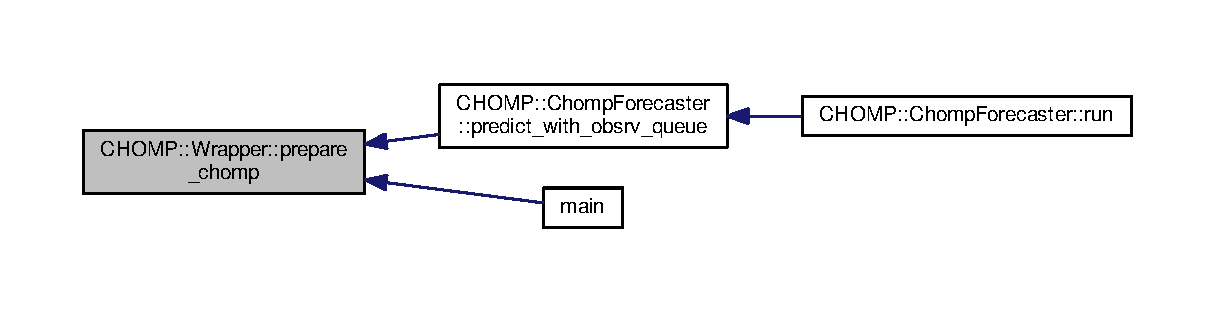
\includegraphics[width=350pt]{class_c_h_o_m_p_1_1_wrapper_a138ac0d5088055c3698d93bbf9432126_icgraph}
\end{center}
\end{figure}


\index{C\+H\+O\+M\+P\+::\+Wrapper@{C\+H\+O\+M\+P\+::\+Wrapper}!publish\+\_\+routine@{publish\+\_\+routine}}
\index{publish\+\_\+routine@{publish\+\_\+routine}!C\+H\+O\+M\+P\+::\+Wrapper@{C\+H\+O\+M\+P\+::\+Wrapper}}
\subsubsection[{\texorpdfstring{publish\+\_\+routine()}{publish_routine()}}]{\setlength{\rightskip}{0pt plus 5cm}void Wrapper\+::publish\+\_\+routine (
\begin{DoxyParamCaption}
{}
\end{DoxyParamCaption}
)}\hypertarget{class_c_h_o_m_p_1_1_wrapper_a84f5c4690636e65aca526e6e5b8abcf4}{}\label{class_c_h_o_m_p_1_1_wrapper_a84f5c4690636e65aca526e6e5b8abcf4}


Definition at line 279 of file chomp\+\_\+ros\+\_\+wrapper.\+cpp.



Here is the caller graph for this function\+:
\nopagebreak
\begin{figure}[H]
\begin{center}
\leavevmode
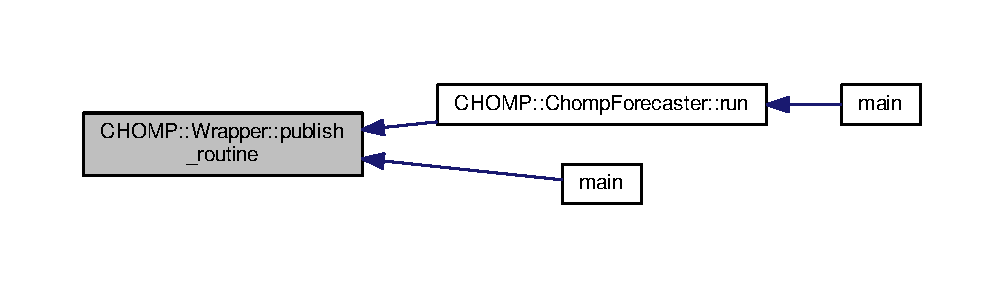
\includegraphics[width=350pt]{class_c_h_o_m_p_1_1_wrapper_a84f5c4690636e65aca526e6e5b8abcf4_icgraph}
\end{center}
\end{figure}


\index{C\+H\+O\+M\+P\+::\+Wrapper@{C\+H\+O\+M\+P\+::\+Wrapper}!solve\+\_\+chomp@{solve\+\_\+chomp}}
\index{solve\+\_\+chomp@{solve\+\_\+chomp}!C\+H\+O\+M\+P\+::\+Wrapper@{C\+H\+O\+M\+P\+::\+Wrapper}}
\subsubsection[{\texorpdfstring{solve\+\_\+chomp(\+Vector\+Xd x0)}{solve_chomp(VectorXd x0)}}]{\setlength{\rightskip}{0pt plus 5cm}bool Wrapper\+::solve\+\_\+chomp (
\begin{DoxyParamCaption}
\item[{Vector\+Xd}]{x0}
\end{DoxyParamCaption}
)}\hypertarget{class_c_h_o_m_p_1_1_wrapper_ac8fa793a31b7872feccc711c55c1da20}{}\label{class_c_h_o_m_p_1_1_wrapper_ac8fa793a31b7872feccc711c55c1da20}


Definition at line 240 of file chomp\+\_\+ros\+\_\+wrapper.\+cpp.



Here is the call graph for this function\+:
\nopagebreak
\begin{figure}[H]
\begin{center}
\leavevmode
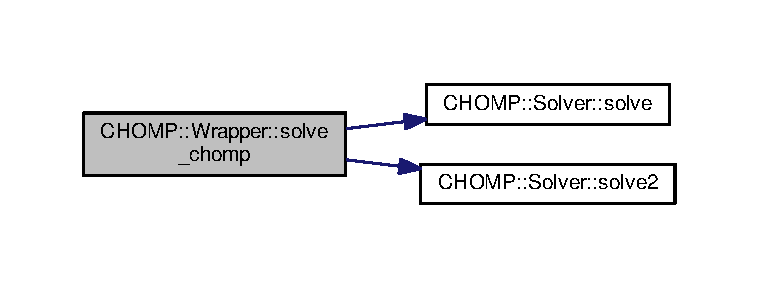
\includegraphics[width=350pt]{class_c_h_o_m_p_1_1_wrapper_ac8fa793a31b7872feccc711c55c1da20_cgraph}
\end{center}
\end{figure}




Here is the caller graph for this function\+:
\nopagebreak
\begin{figure}[H]
\begin{center}
\leavevmode
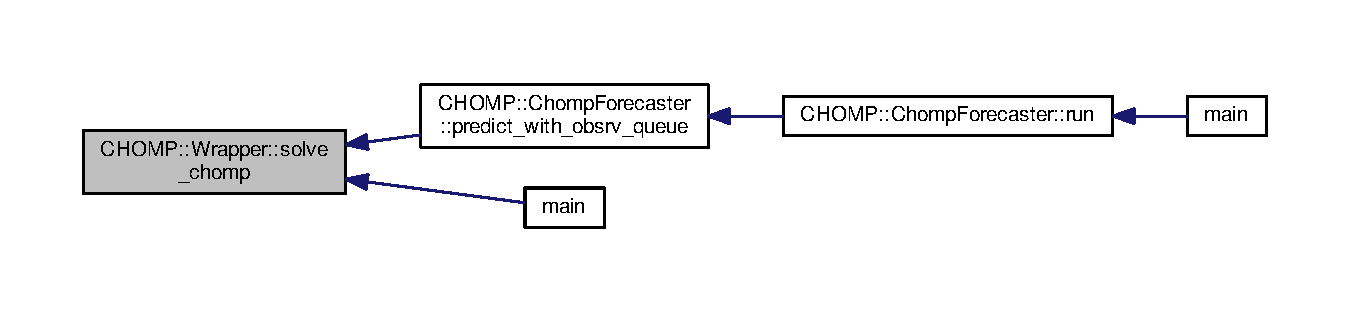
\includegraphics[width=350pt]{class_c_h_o_m_p_1_1_wrapper_ac8fa793a31b7872feccc711c55c1da20_icgraph}
\end{center}
\end{figure}




\subsection{Member Data Documentation}
\index{C\+H\+O\+M\+P\+::\+Wrapper@{C\+H\+O\+M\+P\+::\+Wrapper}!map\+\_\+type@{map\+\_\+type}}
\index{map\+\_\+type@{map\+\_\+type}!C\+H\+O\+M\+P\+::\+Wrapper@{C\+H\+O\+M\+P\+::\+Wrapper}}
\subsubsection[{\texorpdfstring{map\+\_\+type}{map_type}}]{\setlength{\rightskip}{0pt plus 5cm}int C\+H\+O\+M\+P\+::\+Wrapper\+::map\+\_\+type}\hypertarget{class_c_h_o_m_p_1_1_wrapper_a8e7d4dd9f8678e2752ef05e55a36ffe1}{}\label{class_c_h_o_m_p_1_1_wrapper_a8e7d4dd9f8678e2752ef05e55a36ffe1}


Definition at line 49 of file chomp\+\_\+ros\+\_\+wrapper.\+h.

\index{C\+H\+O\+M\+P\+::\+Wrapper@{C\+H\+O\+M\+P\+::\+Wrapper}!recent\+\_\+optim\+\_\+result@{recent\+\_\+optim\+\_\+result}}
\index{recent\+\_\+optim\+\_\+result@{recent\+\_\+optim\+\_\+result}!C\+H\+O\+M\+P\+::\+Wrapper@{C\+H\+O\+M\+P\+::\+Wrapper}}
\subsubsection[{\texorpdfstring{recent\+\_\+optim\+\_\+result}{recent_optim_result}}]{\setlength{\rightskip}{0pt plus 5cm}{\bf Optim\+Result} C\+H\+O\+M\+P\+::\+Wrapper\+::recent\+\_\+optim\+\_\+result}\hypertarget{class_c_h_o_m_p_1_1_wrapper_a5b349bddf6965d721705e451601687a7}{}\label{class_c_h_o_m_p_1_1_wrapper_a5b349bddf6965d721705e451601687a7}


Definition at line 47 of file chomp\+\_\+ros\+\_\+wrapper.\+h.



The documentation for this class was generated from the following files\+:\begin{DoxyCompactItemize}
\item 
include/chomp\+\_\+predict/\hyperlink{chomp__ros__wrapper_8h}{chomp\+\_\+ros\+\_\+wrapper.\+h}\item 
src/\hyperlink{chomp__ros__wrapper_8cpp}{chomp\+\_\+ros\+\_\+wrapper.\+cpp}\end{DoxyCompactItemize}

\chapter{File Documentation}
\hypertarget{generate__cached__setup_8py}{}\section{build/catkin\+\_\+generated/generate\+\_\+cached\+\_\+setup.py File Reference}
\label{generate__cached__setup_8py}\index{build/catkin\+\_\+generated/generate\+\_\+cached\+\_\+setup.\+py@{build/catkin\+\_\+generated/generate\+\_\+cached\+\_\+setup.\+py}}
\subsection*{Namespaces}
\begin{DoxyCompactItemize}
\item 
 \hyperlink{namespacegenerate__cached__setup}{generate\+\_\+cached\+\_\+setup}
\end{DoxyCompactItemize}
\subsection*{Variables}
\begin{DoxyCompactItemize}
\item 
\hyperlink{namespacegenerate__cached__setup_a72579fd01529a79bab20d99291889d3f}{generate\+\_\+cached\+\_\+setup.\+python\+\_\+path} = os.\+path.\+join(workspace, \textquotesingle{}lib/python2.\+7/dist-\/packages\textquotesingle{})
\item 
\hyperlink{namespacegenerate__cached__setup_a52601295006f2366a311c4453d8f2f2e}{generate\+\_\+cached\+\_\+setup.\+code} = generate\+\_\+environment\+\_\+script(\textquotesingle{}/home/jbs/catkin\+\_\+ws/src/chomp\+\_\+predict/build/devel/env.\+sh\textquotesingle{})
\item 
string \hyperlink{namespacegenerate__cached__setup_a0265aee5075ee1eb701ff69c98ad6793}{generate\+\_\+cached\+\_\+setup.\+output\+\_\+filename} = \textquotesingle{}/home/jbs/catkin\+\_\+ws/src/chomp\+\_\+predict/build/catkin\+\_\+generated/setup\+\_\+cached.\+sh\textquotesingle{}
\item 
\hyperlink{namespacegenerate__cached__setup_a10081e5abedae9bd46dd91202096e789}{generate\+\_\+cached\+\_\+setup.\+mode} = os.\+stat(output\+\_\+filename).st\+\_\+mode
\end{DoxyCompactItemize}

\hypertarget{catkin__generated_2installspace_2__setup__util_8py}{}\section{build/catkin\+\_\+generated/installspace/\+\_\+setup\+\_\+util.py File Reference}
\label{catkin__generated_2installspace_2__setup__util_8py}\index{build/catkin\+\_\+generated/installspace/\+\_\+setup\+\_\+util.\+py@{build/catkin\+\_\+generated/installspace/\+\_\+setup\+\_\+util.\+py}}
\subsection*{Namespaces}
\begin{DoxyCompactItemize}
\item 
 \hyperlink{namespace__setup__util}{\+\_\+setup\+\_\+util}
\end{DoxyCompactItemize}
\subsection*{Functions}
\begin{DoxyCompactItemize}
\item 
def \hyperlink{namespace__setup__util_af3030db6102b5aa35cd354a2fb6cca03}{\+\_\+setup\+\_\+util.\+rollback\+\_\+env\+\_\+variables} (environ, env\+\_\+var\+\_\+subfolders)
\item 
def \hyperlink{namespace__setup__util_a832417d18b85bd1d276a87547e86f860}{\+\_\+setup\+\_\+util.\+prepend\+\_\+env\+\_\+variables} (environ, env\+\_\+var\+\_\+subfolders, workspaces)
\item 
def \hyperlink{namespace__setup__util_ad56c24837fa4eddc63c03fbc7035628f}{\+\_\+setup\+\_\+util.\+assignment} (key, value)
\item 
def \hyperlink{namespace__setup__util_abe8c95c4cfe8b1374dacd5f91d984353}{\+\_\+setup\+\_\+util.\+comment} (msg)
\item 
def \hyperlink{namespace__setup__util_ae78d86b2c4279f5b8b1acaa146c35802}{\+\_\+setup\+\_\+util.\+prepend} (environ, key, prefix)
\item 
def \hyperlink{namespace__setup__util_a73de35ca77f260af6691470342ab49ce}{\+\_\+setup\+\_\+util.\+find\+\_\+env\+\_\+hooks} (environ, cmake\+\_\+prefix\+\_\+path)
\end{DoxyCompactItemize}
\subsection*{Variables}
\begin{DoxyCompactItemize}
\item 
string \hyperlink{namespace__setup__util_a3fa0ca5a460a71a43cbc3d4954ab1f10}{\+\_\+setup\+\_\+util.\+C\+A\+T\+K\+I\+N\+\_\+\+M\+A\+R\+K\+E\+R\+\_\+\+F\+I\+LE} = \textquotesingle{}.catkin\textquotesingle{}
\item 
\hyperlink{namespace__setup__util_ae9fca6a80a6923f4580be72f68fee325}{\+\_\+setup\+\_\+util.\+system} = platform.\+system()
\item 
tuple \hyperlink{namespace__setup__util_aecbb100ce6f94bb3c7e16d58fde05f96}{\+\_\+setup\+\_\+util.\+I\+S\+\_\+\+D\+A\+R\+W\+IN} = (system == \textquotesingle{}Darwin\textquotesingle{})
\item 
tuple \hyperlink{namespace__setup__util_a6fe69c2dbd92959b6651a28cbb846e6e}{\+\_\+setup\+\_\+util.\+I\+S\+\_\+\+W\+I\+N\+D\+O\+WS} = (system == \textquotesingle{}Windows\textquotesingle{})
\item 
dictionary \hyperlink{namespace__setup__util_aa31804f1be8660156ce9394b33c68dc4}{\+\_\+setup\+\_\+util.\+E\+N\+V\+\_\+\+V\+A\+R\+\_\+\+S\+U\+B\+F\+O\+L\+D\+E\+RS}
\item 
\hyperlink{namespace__setup__util_a547963d07c6371df1c51b1384a2dec28}{\+\_\+setup\+\_\+util.\+args} = \+\_\+parse\+\_\+arguments()
\item 
\hyperlink{namespace__setup__util_acdce690b925de33d6249bbbfa1109d61}{\+\_\+setup\+\_\+util.\+e}
\item 
\hyperlink{namespace__setup__util_aea63a1b32cc79bc3d872ab7cb30dd07e}{\+\_\+setup\+\_\+util.\+file}
\item 
string \hyperlink{namespace__setup__util_a57afd3d2c076955fb715f3e72ef098eb}{\+\_\+setup\+\_\+util.\+C\+M\+A\+K\+E\+\_\+\+P\+R\+E\+F\+I\+X\+\_\+\+P\+A\+TH} = \textquotesingle{}/home/jbs/catkin\+\_\+ws/devel;/opt/ros/kinetic\textquotesingle{}
\item 
\hyperlink{namespace__setup__util_a83d25140acd7788bbcb95843fe38e639}{\+\_\+setup\+\_\+util.\+base\+\_\+path} = os.\+path.\+dirname(\+\_\+\+\_\+file\+\_\+\+\_\+)
\item 
\hyperlink{namespace__setup__util_a9a935bdd9ee1aa0327161025bb18c136}{\+\_\+setup\+\_\+util.\+environ} = dict(os.\+environ)
\item 
list \hyperlink{namespace__setup__util_a8618d8be5f729d4c9696daa5e083a001}{\+\_\+setup\+\_\+util.\+lines} = \mbox{[}$\,$\mbox{]}
\end{DoxyCompactItemize}

\hypertarget{devel_2__setup__util_8py}{}\section{build/devel/\+\_\+setup\+\_\+util.py File Reference}
\label{devel_2__setup__util_8py}\index{build/devel/\+\_\+setup\+\_\+util.\+py@{build/devel/\+\_\+setup\+\_\+util.\+py}}
\subsection*{Namespaces}
\begin{DoxyCompactItemize}
\item 
 \hyperlink{namespace__setup__util}{\+\_\+setup\+\_\+util}
\end{DoxyCompactItemize}
\subsection*{Functions}
\begin{DoxyCompactItemize}
\item 
def \hyperlink{namespace__setup__util_af3030db6102b5aa35cd354a2fb6cca03}{\+\_\+setup\+\_\+util.\+rollback\+\_\+env\+\_\+variables} (environ, env\+\_\+var\+\_\+subfolders)
\item 
def \hyperlink{namespace__setup__util_a832417d18b85bd1d276a87547e86f860}{\+\_\+setup\+\_\+util.\+prepend\+\_\+env\+\_\+variables} (environ, env\+\_\+var\+\_\+subfolders, workspaces)
\item 
def \hyperlink{namespace__setup__util_ad56c24837fa4eddc63c03fbc7035628f}{\+\_\+setup\+\_\+util.\+assignment} (key, value)
\item 
def \hyperlink{namespace__setup__util_abe8c95c4cfe8b1374dacd5f91d984353}{\+\_\+setup\+\_\+util.\+comment} (msg)
\item 
def \hyperlink{namespace__setup__util_ae78d86b2c4279f5b8b1acaa146c35802}{\+\_\+setup\+\_\+util.\+prepend} (environ, key, prefix)
\item 
def \hyperlink{namespace__setup__util_a73de35ca77f260af6691470342ab49ce}{\+\_\+setup\+\_\+util.\+find\+\_\+env\+\_\+hooks} (environ, cmake\+\_\+prefix\+\_\+path)
\end{DoxyCompactItemize}

\hypertarget{pkg_8develspace_8context_8pc_8py}{}\section{build/catkin\+\_\+generated/pkg.develspace.\+context.\+pc.\+py File Reference}
\label{pkg_8develspace_8context_8pc_8py}\index{build/catkin\+\_\+generated/pkg.\+develspace.\+context.\+pc.\+py@{build/catkin\+\_\+generated/pkg.\+develspace.\+context.\+pc.\+py}}
\subsection*{Namespaces}
\begin{DoxyCompactItemize}
\item 
 \hyperlink{namespacepkg}{pkg}
\end{DoxyCompactItemize}
\subsection*{Variables}
\begin{DoxyCompactItemize}
\item 
string \hyperlink{namespacepkg_ae26c7a5a06b7d738f4d210ca449e6bee}{pkg.\+C\+A\+T\+K\+I\+N\+\_\+\+P\+A\+C\+K\+A\+G\+E\+\_\+\+P\+R\+E\+F\+IX} = \char`\"{}\char`\"{}
\item 
string \hyperlink{namespacepkg_a2760bf8266ff58da440f65ee91b203ab}{pkg.\+P\+R\+O\+J\+E\+C\+T\+\_\+\+P\+K\+G\+\_\+\+C\+O\+N\+F\+I\+G\+\_\+\+I\+N\+C\+L\+U\+D\+E\+\_\+\+D\+I\+RS} = \char`\"{}/home/jbs/catkin\+\_\+ws/src/chomp\+\_\+predict/include\char`\"{}
\item 
string \hyperlink{namespacepkg_a17c18447fad253ee1c0d76deec88028c}{pkg.\+P\+R\+O\+J\+E\+C\+T\+\_\+\+C\+A\+T\+K\+I\+N\+\_\+\+D\+E\+P\+E\+N\+DS} = \char`\"{}\char`\"{}
\item 
string \hyperlink{namespacepkg_a433e30cecb4a0123a7c4b384d168e336}{pkg.\+P\+K\+G\+\_\+\+C\+O\+N\+F\+I\+G\+\_\+\+L\+I\+B\+R\+A\+R\+I\+E\+S\+\_\+\+W\+I\+T\+H\+\_\+\+P\+R\+E\+F\+IX} = \char`\"{}-\/lchomp\+\_\+predict\char`\"{}
\item 
string \hyperlink{namespacepkg_a7dfbe99257c26f5e4a3a5483995d9ddc}{pkg.\+P\+R\+O\+J\+E\+C\+T\+\_\+\+N\+A\+ME} = \char`\"{}chomp\+\_\+predict\char`\"{}
\item 
string \hyperlink{namespacepkg_a3f0f1b4bc03c596525e025539ca4332f}{pkg.\+P\+R\+O\+J\+E\+C\+T\+\_\+\+S\+P\+A\+C\+E\+\_\+\+D\+IR} = \char`\"{}/home/jbs/catkin\+\_\+ws/src/chomp\+\_\+predict/build/devel\char`\"{}
\item 
string \hyperlink{namespacepkg_ab1037914b9286bb61855131c06149648}{pkg.\+P\+R\+O\+J\+E\+C\+T\+\_\+\+V\+E\+R\+S\+I\+ON} = \char`\"{}0.\+0.\+0\char`\"{}
\end{DoxyCompactItemize}

\hypertarget{pkg_8installspace_8context_8pc_8py}{}\section{build/catkin\+\_\+generated/pkg.installspace.\+context.\+pc.\+py File Reference}
\label{pkg_8installspace_8context_8pc_8py}\index{build/catkin\+\_\+generated/pkg.\+installspace.\+context.\+pc.\+py@{build/catkin\+\_\+generated/pkg.\+installspace.\+context.\+pc.\+py}}
\subsection*{Namespaces}
\begin{DoxyCompactItemize}
\item 
 \hyperlink{namespacepkg}{pkg}
\end{DoxyCompactItemize}

\hypertarget{_c_make_c_compiler_id_8c}{}\section{build/\+C\+Make\+Files/3.5.1/\+Compiler\+Id\+C/\+C\+Make\+C\+Compiler\+Id.c File Reference}
\label{_c_make_c_compiler_id_8c}\index{build/\+C\+Make\+Files/3.\+5.\+1/\+Compiler\+Id\+C/\+C\+Make\+C\+Compiler\+Id.\+c@{build/\+C\+Make\+Files/3.\+5.\+1/\+Compiler\+Id\+C/\+C\+Make\+C\+Compiler\+Id.\+c}}
\subsection*{Macros}
\begin{DoxyCompactItemize}
\item 
\#define \hyperlink{_c_make_c_compiler_id_8c_a81dee0709ded976b2e0319239f72d174}{C\+O\+M\+P\+I\+L\+E\+R\+\_\+\+ID}~\char`\"{}\char`\"{}
\item 
\#define \hyperlink{_c_make_c_compiler_id_8c_a2ae9b72bb13abaabfcf2ee0ba7d3fa1d}{S\+T\+R\+I\+N\+G\+I\+F\+Y\+\_\+\+H\+E\+L\+P\+ER}(X)~\#X
\item 
\#define \hyperlink{_c_make_c_compiler_id_8c_a43e1cad902b6477bec893cb6430bd6c8}{S\+T\+R\+I\+N\+G\+I\+FY}(X)~\hyperlink{_c_make_c_x_x_compiler_id_8cpp_a2ae9b72bb13abaabfcf2ee0ba7d3fa1d}{S\+T\+R\+I\+N\+G\+I\+F\+Y\+\_\+\+H\+E\+L\+P\+ER}(X)
\item 
\#define \hyperlink{_c_make_c_compiler_id_8c_adbc5372f40838899018fadbc89bd588b}{P\+L\+A\+T\+F\+O\+R\+M\+\_\+\+ID}~\char`\"{}\char`\"{}
\item 
\#define \hyperlink{_c_make_c_compiler_id_8c_aba35d0d200deaeb06aee95ca297acb28}{A\+R\+C\+H\+I\+T\+E\+C\+T\+U\+R\+E\+\_\+\+ID}~\char`\"{}\char`\"{}
\item 
\#define \hyperlink{_c_make_c_compiler_id_8c_ad1280362da42492bbc11aa78cbf776ad}{D\+EC}(n)
\item 
\#define \hyperlink{_c_make_c_compiler_id_8c_a46d5d95daa1bef867bd0179594310ed5}{H\+EX}(n)
\end{DoxyCompactItemize}
\subsection*{Functions}
\begin{DoxyCompactItemize}
\item 
int \hyperlink{_c_make_c_compiler_id_8c_a0ddf1224851353fc92bfbff6f499fa97}{main} (int argc, char $\ast$argv\mbox{[}$\,$\mbox{]})
\end{DoxyCompactItemize}
\subsection*{Variables}
\begin{DoxyCompactItemize}
\item 
char const $\ast$ \hyperlink{_c_make_c_compiler_id_8c_a4b0efeb7a5d59313986b3a0390f050f6}{info\+\_\+compiler} = \char`\"{}I\+N\+FO\char`\"{} \char`\"{}\+:\char`\"{} \char`\"{}compiler\mbox{[}\char`\"{} C\+O\+M\+P\+I\+L\+E\+R\+\_\+\+ID \char`\"{}\mbox{]}\char`\"{}
\item 
char const $\ast$ \hyperlink{_c_make_c_compiler_id_8c_a2321403dee54ee23f0c2fa849c60f7d4}{info\+\_\+platform} = \char`\"{}I\+N\+FO\char`\"{} \char`\"{}\+:\char`\"{} \char`\"{}platform\mbox{[}\char`\"{} P\+L\+A\+T\+F\+O\+R\+M\+\_\+\+ID \char`\"{}\mbox{]}\char`\"{}
\item 
char const $\ast$ \hyperlink{_c_make_c_compiler_id_8c_a59647e99d304ed33b15cb284c27ed391}{info\+\_\+arch} = \char`\"{}I\+N\+FO\char`\"{} \char`\"{}\+:\char`\"{} \char`\"{}arch\mbox{[}\char`\"{} A\+R\+C\+H\+I\+T\+E\+C\+T\+U\+R\+E\+\_\+\+ID \char`\"{}\mbox{]}\char`\"{}
\item 
const char $\ast$ \hyperlink{_c_make_c_compiler_id_8c_a1ce162bad2fe6966ac8b33cc19e120b8}{info\+\_\+language\+\_\+dialect\+\_\+default}
\end{DoxyCompactItemize}


\subsection{Macro Definition Documentation}
\index{C\+Make\+C\+Compiler\+Id.\+c@{C\+Make\+C\+Compiler\+Id.\+c}!A\+R\+C\+H\+I\+T\+E\+C\+T\+U\+R\+E\+\_\+\+ID@{A\+R\+C\+H\+I\+T\+E\+C\+T\+U\+R\+E\+\_\+\+ID}}
\index{A\+R\+C\+H\+I\+T\+E\+C\+T\+U\+R\+E\+\_\+\+ID@{A\+R\+C\+H\+I\+T\+E\+C\+T\+U\+R\+E\+\_\+\+ID}!C\+Make\+C\+Compiler\+Id.\+c@{C\+Make\+C\+Compiler\+Id.\+c}}
\subsubsection[{\texorpdfstring{A\+R\+C\+H\+I\+T\+E\+C\+T\+U\+R\+E\+\_\+\+ID}{ARCHITECTURE_ID}}]{\setlength{\rightskip}{0pt plus 5cm}\#define A\+R\+C\+H\+I\+T\+E\+C\+T\+U\+R\+E\+\_\+\+ID~\char`\"{}\char`\"{}}\hypertarget{_c_make_c_compiler_id_8c_aba35d0d200deaeb06aee95ca297acb28}{}\label{_c_make_c_compiler_id_8c_aba35d0d200deaeb06aee95ca297acb28}


Definition at line 435 of file C\+Make\+C\+Compiler\+Id.\+c.

\index{C\+Make\+C\+Compiler\+Id.\+c@{C\+Make\+C\+Compiler\+Id.\+c}!C\+O\+M\+P\+I\+L\+E\+R\+\_\+\+ID@{C\+O\+M\+P\+I\+L\+E\+R\+\_\+\+ID}}
\index{C\+O\+M\+P\+I\+L\+E\+R\+\_\+\+ID@{C\+O\+M\+P\+I\+L\+E\+R\+\_\+\+ID}!C\+Make\+C\+Compiler\+Id.\+c@{C\+Make\+C\+Compiler\+Id.\+c}}
\subsubsection[{\texorpdfstring{C\+O\+M\+P\+I\+L\+E\+R\+\_\+\+ID}{COMPILER_ID}}]{\setlength{\rightskip}{0pt plus 5cm}\#define C\+O\+M\+P\+I\+L\+E\+R\+\_\+\+ID~\char`\"{}\char`\"{}}\hypertarget{_c_make_c_compiler_id_8c_a81dee0709ded976b2e0319239f72d174}{}\label{_c_make_c_compiler_id_8c_a81dee0709ded976b2e0319239f72d174}


Definition at line 268 of file C\+Make\+C\+Compiler\+Id.\+c.

\index{C\+Make\+C\+Compiler\+Id.\+c@{C\+Make\+C\+Compiler\+Id.\+c}!D\+EC@{D\+EC}}
\index{D\+EC@{D\+EC}!C\+Make\+C\+Compiler\+Id.\+c@{C\+Make\+C\+Compiler\+Id.\+c}}
\subsubsection[{\texorpdfstring{D\+EC}{DEC}}]{\setlength{\rightskip}{0pt plus 5cm}\#define D\+EC(
\begin{DoxyParamCaption}
\item[{}]{n}
\end{DoxyParamCaption}
)}\hypertarget{_c_make_c_compiler_id_8c_ad1280362da42492bbc11aa78cbf776ad}{}\label{_c_make_c_compiler_id_8c_ad1280362da42492bbc11aa78cbf776ad}
{\bfseries Value\+:}
\begin{DoxyCode}
(\textcolor{charliteral}{'0'} + (((n) / 10000000)%10)), \(\backslash\)
  (\textcolor{charliteral}{'0'} + (((n) / 1000000)%10)),  \(\backslash\)
  (\textcolor{charliteral}{'0'} + (((n) / 100000)%10)),   \(\backslash\)
  (\textcolor{charliteral}{'0'} + (((n) / 10000)%10)),    \(\backslash\)
  (\textcolor{charliteral}{'0'} + (((n) / 1000)%10)),     \(\backslash\)
  (\textcolor{charliteral}{'0'} + (((n) / 100)%10)),      \(\backslash\)
  (\textcolor{charliteral}{'0'} + (((n) / 10)%10)),       \(\backslash\)
  (\textcolor{charliteral}{'0'} +  ((n) % 10))
\end{DoxyCode}


Definition at line 439 of file C\+Make\+C\+Compiler\+Id.\+c.

\index{C\+Make\+C\+Compiler\+Id.\+c@{C\+Make\+C\+Compiler\+Id.\+c}!H\+EX@{H\+EX}}
\index{H\+EX@{H\+EX}!C\+Make\+C\+Compiler\+Id.\+c@{C\+Make\+C\+Compiler\+Id.\+c}}
\subsubsection[{\texorpdfstring{H\+EX}{HEX}}]{\setlength{\rightskip}{0pt plus 5cm}\#define H\+EX(
\begin{DoxyParamCaption}
\item[{}]{n}
\end{DoxyParamCaption}
)}\hypertarget{_c_make_c_compiler_id_8c_a46d5d95daa1bef867bd0179594310ed5}{}\label{_c_make_c_compiler_id_8c_a46d5d95daa1bef867bd0179594310ed5}
{\bfseries Value\+:}
\begin{DoxyCode}
(\textcolor{charliteral}{'0'} + ((n)>>28 & 0xF)), \(\backslash\)
  (\textcolor{charliteral}{'0'} + ((n)>>24 & 0xF)), \(\backslash\)
  (\textcolor{charliteral}{'0'} + ((n)>>20 & 0xF)), \(\backslash\)
  (\textcolor{charliteral}{'0'} + ((n)>>16 & 0xF)), \(\backslash\)
  (\textcolor{charliteral}{'0'} + ((n)>>12 & 0xF)), \(\backslash\)
  (\textcolor{charliteral}{'0'} + ((n)>>8  & 0xF)), \(\backslash\)
  (\textcolor{charliteral}{'0'} + ((n)>>4  & 0xF)), \(\backslash\)
  (\textcolor{charliteral}{'0'} + ((n)     & 0xF))
\end{DoxyCode}


Definition at line 450 of file C\+Make\+C\+Compiler\+Id.\+c.

\index{C\+Make\+C\+Compiler\+Id.\+c@{C\+Make\+C\+Compiler\+Id.\+c}!P\+L\+A\+T\+F\+O\+R\+M\+\_\+\+ID@{P\+L\+A\+T\+F\+O\+R\+M\+\_\+\+ID}}
\index{P\+L\+A\+T\+F\+O\+R\+M\+\_\+\+ID@{P\+L\+A\+T\+F\+O\+R\+M\+\_\+\+ID}!C\+Make\+C\+Compiler\+Id.\+c@{C\+Make\+C\+Compiler\+Id.\+c}}
\subsubsection[{\texorpdfstring{P\+L\+A\+T\+F\+O\+R\+M\+\_\+\+ID}{PLATFORM_ID}}]{\setlength{\rightskip}{0pt plus 5cm}\#define P\+L\+A\+T\+F\+O\+R\+M\+\_\+\+ID~\char`\"{}\char`\"{}}\hypertarget{_c_make_c_compiler_id_8c_adbc5372f40838899018fadbc89bd588b}{}\label{_c_make_c_compiler_id_8c_adbc5372f40838899018fadbc89bd588b}


Definition at line 385 of file C\+Make\+C\+Compiler\+Id.\+c.

\index{C\+Make\+C\+Compiler\+Id.\+c@{C\+Make\+C\+Compiler\+Id.\+c}!S\+T\+R\+I\+N\+G\+I\+FY@{S\+T\+R\+I\+N\+G\+I\+FY}}
\index{S\+T\+R\+I\+N\+G\+I\+FY@{S\+T\+R\+I\+N\+G\+I\+FY}!C\+Make\+C\+Compiler\+Id.\+c@{C\+Make\+C\+Compiler\+Id.\+c}}
\subsubsection[{\texorpdfstring{S\+T\+R\+I\+N\+G\+I\+FY}{STRINGIFY}}]{\setlength{\rightskip}{0pt plus 5cm}\#define S\+T\+R\+I\+N\+G\+I\+FY(
\begin{DoxyParamCaption}
\item[{}]{X}
\end{DoxyParamCaption}
)~{\bf S\+T\+R\+I\+N\+G\+I\+F\+Y\+\_\+\+H\+E\+L\+P\+ER}(X)}\hypertarget{_c_make_c_compiler_id_8c_a43e1cad902b6477bec893cb6430bd6c8}{}\label{_c_make_c_compiler_id_8c_a43e1cad902b6477bec893cb6430bd6c8}


Definition at line 289 of file C\+Make\+C\+Compiler\+Id.\+c.

\index{C\+Make\+C\+Compiler\+Id.\+c@{C\+Make\+C\+Compiler\+Id.\+c}!S\+T\+R\+I\+N\+G\+I\+F\+Y\+\_\+\+H\+E\+L\+P\+ER@{S\+T\+R\+I\+N\+G\+I\+F\+Y\+\_\+\+H\+E\+L\+P\+ER}}
\index{S\+T\+R\+I\+N\+G\+I\+F\+Y\+\_\+\+H\+E\+L\+P\+ER@{S\+T\+R\+I\+N\+G\+I\+F\+Y\+\_\+\+H\+E\+L\+P\+ER}!C\+Make\+C\+Compiler\+Id.\+c@{C\+Make\+C\+Compiler\+Id.\+c}}
\subsubsection[{\texorpdfstring{S\+T\+R\+I\+N\+G\+I\+F\+Y\+\_\+\+H\+E\+L\+P\+ER}{STRINGIFY_HELPER}}]{\setlength{\rightskip}{0pt plus 5cm}\#define S\+T\+R\+I\+N\+G\+I\+F\+Y\+\_\+\+H\+E\+L\+P\+ER(
\begin{DoxyParamCaption}
\item[{}]{X}
\end{DoxyParamCaption}
)~\#X}\hypertarget{_c_make_c_compiler_id_8c_a2ae9b72bb13abaabfcf2ee0ba7d3fa1d}{}\label{_c_make_c_compiler_id_8c_a2ae9b72bb13abaabfcf2ee0ba7d3fa1d}


Definition at line 288 of file C\+Make\+C\+Compiler\+Id.\+c.



\subsection{Function Documentation}
\index{C\+Make\+C\+Compiler\+Id.\+c@{C\+Make\+C\+Compiler\+Id.\+c}!main@{main}}
\index{main@{main}!C\+Make\+C\+Compiler\+Id.\+c@{C\+Make\+C\+Compiler\+Id.\+c}}
\subsubsection[{\texorpdfstring{main(int argc, char $\ast$argv[])}{main(int argc, char *argv[])}}]{\setlength{\rightskip}{0pt plus 5cm}int main (
\begin{DoxyParamCaption}
\item[{int}]{argc, }
\item[{char $\ast$}]{argv\mbox{[}$\,$\mbox{]}}
\end{DoxyParamCaption}
)}\hypertarget{_c_make_c_compiler_id_8c_a0ddf1224851353fc92bfbff6f499fa97}{}\label{_c_make_c_compiler_id_8c_a0ddf1224851353fc92bfbff6f499fa97}


Definition at line 522 of file C\+Make\+C\+Compiler\+Id.\+c.



\subsection{Variable Documentation}
\index{C\+Make\+C\+Compiler\+Id.\+c@{C\+Make\+C\+Compiler\+Id.\+c}!info\+\_\+arch@{info\+\_\+arch}}
\index{info\+\_\+arch@{info\+\_\+arch}!C\+Make\+C\+Compiler\+Id.\+c@{C\+Make\+C\+Compiler\+Id.\+c}}
\subsubsection[{\texorpdfstring{info\+\_\+arch}{info_arch}}]{\setlength{\rightskip}{0pt plus 5cm}char const$\ast$ info\+\_\+arch = \char`\"{}I\+N\+FO\char`\"{} \char`\"{}\+:\char`\"{} \char`\"{}arch\mbox{[}\char`\"{} A\+R\+C\+H\+I\+T\+E\+C\+T\+U\+R\+E\+\_\+\+ID \char`\"{}\mbox{]}\char`\"{}}\hypertarget{_c_make_c_compiler_id_8c_a59647e99d304ed33b15cb284c27ed391}{}\label{_c_make_c_compiler_id_8c_a59647e99d304ed33b15cb284c27ed391}


Definition at line 501 of file C\+Make\+C\+Compiler\+Id.\+c.

\index{C\+Make\+C\+Compiler\+Id.\+c@{C\+Make\+C\+Compiler\+Id.\+c}!info\+\_\+compiler@{info\+\_\+compiler}}
\index{info\+\_\+compiler@{info\+\_\+compiler}!C\+Make\+C\+Compiler\+Id.\+c@{C\+Make\+C\+Compiler\+Id.\+c}}
\subsubsection[{\texorpdfstring{info\+\_\+compiler}{info_compiler}}]{\setlength{\rightskip}{0pt plus 5cm}char const$\ast$ info\+\_\+compiler = \char`\"{}I\+N\+FO\char`\"{} \char`\"{}\+:\char`\"{} \char`\"{}compiler\mbox{[}\char`\"{} C\+O\+M\+P\+I\+L\+E\+R\+\_\+\+ID \char`\"{}\mbox{]}\char`\"{}}\hypertarget{_c_make_c_compiler_id_8c_a4b0efeb7a5d59313986b3a0390f050f6}{}\label{_c_make_c_compiler_id_8c_a4b0efeb7a5d59313986b3a0390f050f6}


Definition at line 275 of file C\+Make\+C\+Compiler\+Id.\+c.

\index{C\+Make\+C\+Compiler\+Id.\+c@{C\+Make\+C\+Compiler\+Id.\+c}!info\+\_\+language\+\_\+dialect\+\_\+default@{info\+\_\+language\+\_\+dialect\+\_\+default}}
\index{info\+\_\+language\+\_\+dialect\+\_\+default@{info\+\_\+language\+\_\+dialect\+\_\+default}!C\+Make\+C\+Compiler\+Id.\+c@{C\+Make\+C\+Compiler\+Id.\+c}}
\subsubsection[{\texorpdfstring{info\+\_\+language\+\_\+dialect\+\_\+default}{info_language_dialect_default}}]{\setlength{\rightskip}{0pt plus 5cm}const char$\ast$ info\+\_\+language\+\_\+dialect\+\_\+default}\hypertarget{_c_make_c_compiler_id_8c_a1ce162bad2fe6966ac8b33cc19e120b8}{}\label{_c_make_c_compiler_id_8c_a1ce162bad2fe6966ac8b33cc19e120b8}
{\bfseries Initial value\+:}
\begin{DoxyCode}
= \textcolor{stringliteral}{"INFO"} \textcolor{stringliteral}{":"} \textcolor{stringliteral}{"dialect\_default["}

  \textcolor{stringliteral}{"90"}






\textcolor{stringliteral}{"]"}
\end{DoxyCode}


Definition at line 506 of file C\+Make\+C\+Compiler\+Id.\+c.

\index{C\+Make\+C\+Compiler\+Id.\+c@{C\+Make\+C\+Compiler\+Id.\+c}!info\+\_\+platform@{info\+\_\+platform}}
\index{info\+\_\+platform@{info\+\_\+platform}!C\+Make\+C\+Compiler\+Id.\+c@{C\+Make\+C\+Compiler\+Id.\+c}}
\subsubsection[{\texorpdfstring{info\+\_\+platform}{info_platform}}]{\setlength{\rightskip}{0pt plus 5cm}char const$\ast$ info\+\_\+platform = \char`\"{}I\+N\+FO\char`\"{} \char`\"{}\+:\char`\"{} \char`\"{}platform\mbox{[}\char`\"{} P\+L\+A\+T\+F\+O\+R\+M\+\_\+\+ID \char`\"{}\mbox{]}\char`\"{}}\hypertarget{_c_make_c_compiler_id_8c_a2321403dee54ee23f0c2fa849c60f7d4}{}\label{_c_make_c_compiler_id_8c_a2321403dee54ee23f0c2fa849c60f7d4}


Definition at line 500 of file C\+Make\+C\+Compiler\+Id.\+c.


\hypertarget{_c_make_c_x_x_compiler_id_8cpp}{}\section{build/\+C\+Make\+Files/3.5.1/\+Compiler\+Id\+C\+X\+X/\+C\+Make\+C\+X\+X\+Compiler\+Id.cpp File Reference}
\label{_c_make_c_x_x_compiler_id_8cpp}\index{build/\+C\+Make\+Files/3.\+5.\+1/\+Compiler\+Id\+C\+X\+X/\+C\+Make\+C\+X\+X\+Compiler\+Id.\+cpp@{build/\+C\+Make\+Files/3.\+5.\+1/\+Compiler\+Id\+C\+X\+X/\+C\+Make\+C\+X\+X\+Compiler\+Id.\+cpp}}
\subsection*{Macros}
\begin{DoxyCompactItemize}
\item 
\#define \hyperlink{_c_make_c_x_x_compiler_id_8cpp_a81dee0709ded976b2e0319239f72d174}{C\+O\+M\+P\+I\+L\+E\+R\+\_\+\+ID}~\char`\"{}\char`\"{}
\item 
\#define \hyperlink{_c_make_c_x_x_compiler_id_8cpp_a2ae9b72bb13abaabfcf2ee0ba7d3fa1d}{S\+T\+R\+I\+N\+G\+I\+F\+Y\+\_\+\+H\+E\+L\+P\+ER}(X)~\#X
\item 
\#define \hyperlink{_c_make_c_x_x_compiler_id_8cpp_a43e1cad902b6477bec893cb6430bd6c8}{S\+T\+R\+I\+N\+G\+I\+FY}(X)~\hyperlink{_c_make_c_x_x_compiler_id_8cpp_a2ae9b72bb13abaabfcf2ee0ba7d3fa1d}{S\+T\+R\+I\+N\+G\+I\+F\+Y\+\_\+\+H\+E\+L\+P\+ER}(X)
\item 
\#define \hyperlink{_c_make_c_x_x_compiler_id_8cpp_adbc5372f40838899018fadbc89bd588b}{P\+L\+A\+T\+F\+O\+R\+M\+\_\+\+ID}~\char`\"{}\char`\"{}
\item 
\#define \hyperlink{_c_make_c_x_x_compiler_id_8cpp_aba35d0d200deaeb06aee95ca297acb28}{A\+R\+C\+H\+I\+T\+E\+C\+T\+U\+R\+E\+\_\+\+ID}~\char`\"{}\char`\"{}
\item 
\#define \hyperlink{_c_make_c_x_x_compiler_id_8cpp_ad1280362da42492bbc11aa78cbf776ad}{D\+EC}(n)
\item 
\#define \hyperlink{_c_make_c_x_x_compiler_id_8cpp_a46d5d95daa1bef867bd0179594310ed5}{H\+EX}(n)
\end{DoxyCompactItemize}
\subsection*{Functions}
\begin{DoxyCompactItemize}
\item 
int \hyperlink{_c_make_c_x_x_compiler_id_8cpp_a0ddf1224851353fc92bfbff6f499fa97}{main} (int argc, char $\ast$argv\mbox{[}$\,$\mbox{]})
\end{DoxyCompactItemize}
\subsection*{Variables}
\begin{DoxyCompactItemize}
\item 
char const $\ast$ \hyperlink{_c_make_c_x_x_compiler_id_8cpp_a4b0efeb7a5d59313986b3a0390f050f6}{info\+\_\+compiler} = \char`\"{}I\+N\+FO\char`\"{} \char`\"{}\+:\char`\"{} \char`\"{}compiler\mbox{[}\char`\"{} C\+O\+M\+P\+I\+L\+E\+R\+\_\+\+ID \char`\"{}\mbox{]}\char`\"{}
\item 
char const $\ast$ \hyperlink{_c_make_c_x_x_compiler_id_8cpp_a2321403dee54ee23f0c2fa849c60f7d4}{info\+\_\+platform} = \char`\"{}I\+N\+FO\char`\"{} \char`\"{}\+:\char`\"{} \char`\"{}platform\mbox{[}\char`\"{} P\+L\+A\+T\+F\+O\+R\+M\+\_\+\+ID \char`\"{}\mbox{]}\char`\"{}
\item 
char const $\ast$ \hyperlink{_c_make_c_x_x_compiler_id_8cpp_a59647e99d304ed33b15cb284c27ed391}{info\+\_\+arch} = \char`\"{}I\+N\+FO\char`\"{} \char`\"{}\+:\char`\"{} \char`\"{}arch\mbox{[}\char`\"{} A\+R\+C\+H\+I\+T\+E\+C\+T\+U\+R\+E\+\_\+\+ID \char`\"{}\mbox{]}\char`\"{}
\item 
const char $\ast$ \hyperlink{_c_make_c_x_x_compiler_id_8cpp_a1ce162bad2fe6966ac8b33cc19e120b8}{info\+\_\+language\+\_\+dialect\+\_\+default}
\end{DoxyCompactItemize}


\subsection{Macro Definition Documentation}
\index{C\+Make\+C\+X\+X\+Compiler\+Id.\+cpp@{C\+Make\+C\+X\+X\+Compiler\+Id.\+cpp}!A\+R\+C\+H\+I\+T\+E\+C\+T\+U\+R\+E\+\_\+\+ID@{A\+R\+C\+H\+I\+T\+E\+C\+T\+U\+R\+E\+\_\+\+ID}}
\index{A\+R\+C\+H\+I\+T\+E\+C\+T\+U\+R\+E\+\_\+\+ID@{A\+R\+C\+H\+I\+T\+E\+C\+T\+U\+R\+E\+\_\+\+ID}!C\+Make\+C\+X\+X\+Compiler\+Id.\+cpp@{C\+Make\+C\+X\+X\+Compiler\+Id.\+cpp}}
\subsubsection[{\texorpdfstring{A\+R\+C\+H\+I\+T\+E\+C\+T\+U\+R\+E\+\_\+\+ID}{ARCHITECTURE_ID}}]{\setlength{\rightskip}{0pt plus 5cm}\#define A\+R\+C\+H\+I\+T\+E\+C\+T\+U\+R\+E\+\_\+\+ID~\char`\"{}\char`\"{}}\hypertarget{_c_make_c_x_x_compiler_id_8cpp_aba35d0d200deaeb06aee95ca297acb28}{}\label{_c_make_c_x_x_compiler_id_8cpp_aba35d0d200deaeb06aee95ca297acb28}


Definition at line 430 of file C\+Make\+C\+X\+X\+Compiler\+Id.\+cpp.

\index{C\+Make\+C\+X\+X\+Compiler\+Id.\+cpp@{C\+Make\+C\+X\+X\+Compiler\+Id.\+cpp}!C\+O\+M\+P\+I\+L\+E\+R\+\_\+\+ID@{C\+O\+M\+P\+I\+L\+E\+R\+\_\+\+ID}}
\index{C\+O\+M\+P\+I\+L\+E\+R\+\_\+\+ID@{C\+O\+M\+P\+I\+L\+E\+R\+\_\+\+ID}!C\+Make\+C\+X\+X\+Compiler\+Id.\+cpp@{C\+Make\+C\+X\+X\+Compiler\+Id.\+cpp}}
\subsubsection[{\texorpdfstring{C\+O\+M\+P\+I\+L\+E\+R\+\_\+\+ID}{COMPILER_ID}}]{\setlength{\rightskip}{0pt plus 5cm}\#define C\+O\+M\+P\+I\+L\+E\+R\+\_\+\+ID~\char`\"{}\char`\"{}}\hypertarget{_c_make_c_x_x_compiler_id_8cpp_a81dee0709ded976b2e0319239f72d174}{}\label{_c_make_c_x_x_compiler_id_8cpp_a81dee0709ded976b2e0319239f72d174}


Definition at line 263 of file C\+Make\+C\+X\+X\+Compiler\+Id.\+cpp.

\index{C\+Make\+C\+X\+X\+Compiler\+Id.\+cpp@{C\+Make\+C\+X\+X\+Compiler\+Id.\+cpp}!D\+EC@{D\+EC}}
\index{D\+EC@{D\+EC}!C\+Make\+C\+X\+X\+Compiler\+Id.\+cpp@{C\+Make\+C\+X\+X\+Compiler\+Id.\+cpp}}
\subsubsection[{\texorpdfstring{D\+EC}{DEC}}]{\setlength{\rightskip}{0pt plus 5cm}\#define D\+EC(
\begin{DoxyParamCaption}
\item[{}]{n}
\end{DoxyParamCaption}
)}\hypertarget{_c_make_c_x_x_compiler_id_8cpp_ad1280362da42492bbc11aa78cbf776ad}{}\label{_c_make_c_x_x_compiler_id_8cpp_ad1280362da42492bbc11aa78cbf776ad}
{\bfseries Value\+:}
\begin{DoxyCode}
(\textcolor{charliteral}{'0'} + (((n) / 10000000)%10)), \(\backslash\)
  (\textcolor{charliteral}{'0'} + (((n) / 1000000)%10)),  \(\backslash\)
  (\textcolor{charliteral}{'0'} + (((n) / 100000)%10)),   \(\backslash\)
  (\textcolor{charliteral}{'0'} + (((n) / 10000)%10)),    \(\backslash\)
  (\textcolor{charliteral}{'0'} + (((n) / 1000)%10)),     \(\backslash\)
  (\textcolor{charliteral}{'0'} + (((n) / 100)%10)),      \(\backslash\)
  (\textcolor{charliteral}{'0'} + (((n) / 10)%10)),       \(\backslash\)
  (\textcolor{charliteral}{'0'} +  ((n) % 10))
\end{DoxyCode}


Definition at line 434 of file C\+Make\+C\+X\+X\+Compiler\+Id.\+cpp.

\index{C\+Make\+C\+X\+X\+Compiler\+Id.\+cpp@{C\+Make\+C\+X\+X\+Compiler\+Id.\+cpp}!H\+EX@{H\+EX}}
\index{H\+EX@{H\+EX}!C\+Make\+C\+X\+X\+Compiler\+Id.\+cpp@{C\+Make\+C\+X\+X\+Compiler\+Id.\+cpp}}
\subsubsection[{\texorpdfstring{H\+EX}{HEX}}]{\setlength{\rightskip}{0pt plus 5cm}\#define H\+EX(
\begin{DoxyParamCaption}
\item[{}]{n}
\end{DoxyParamCaption}
)}\hypertarget{_c_make_c_x_x_compiler_id_8cpp_a46d5d95daa1bef867bd0179594310ed5}{}\label{_c_make_c_x_x_compiler_id_8cpp_a46d5d95daa1bef867bd0179594310ed5}
{\bfseries Value\+:}
\begin{DoxyCode}
(\textcolor{charliteral}{'0'} + ((n)>>28 & 0xF)), \(\backslash\)
  (\textcolor{charliteral}{'0'} + ((n)>>24 & 0xF)), \(\backslash\)
  (\textcolor{charliteral}{'0'} + ((n)>>20 & 0xF)), \(\backslash\)
  (\textcolor{charliteral}{'0'} + ((n)>>16 & 0xF)), \(\backslash\)
  (\textcolor{charliteral}{'0'} + ((n)>>12 & 0xF)), \(\backslash\)
  (\textcolor{charliteral}{'0'} + ((n)>>8  & 0xF)), \(\backslash\)
  (\textcolor{charliteral}{'0'} + ((n)>>4  & 0xF)), \(\backslash\)
  (\textcolor{charliteral}{'0'} + ((n)     & 0xF))
\end{DoxyCode}


Definition at line 445 of file C\+Make\+C\+X\+X\+Compiler\+Id.\+cpp.

\index{C\+Make\+C\+X\+X\+Compiler\+Id.\+cpp@{C\+Make\+C\+X\+X\+Compiler\+Id.\+cpp}!P\+L\+A\+T\+F\+O\+R\+M\+\_\+\+ID@{P\+L\+A\+T\+F\+O\+R\+M\+\_\+\+ID}}
\index{P\+L\+A\+T\+F\+O\+R\+M\+\_\+\+ID@{P\+L\+A\+T\+F\+O\+R\+M\+\_\+\+ID}!C\+Make\+C\+X\+X\+Compiler\+Id.\+cpp@{C\+Make\+C\+X\+X\+Compiler\+Id.\+cpp}}
\subsubsection[{\texorpdfstring{P\+L\+A\+T\+F\+O\+R\+M\+\_\+\+ID}{PLATFORM_ID}}]{\setlength{\rightskip}{0pt plus 5cm}\#define P\+L\+A\+T\+F\+O\+R\+M\+\_\+\+ID~\char`\"{}\char`\"{}}\hypertarget{_c_make_c_x_x_compiler_id_8cpp_adbc5372f40838899018fadbc89bd588b}{}\label{_c_make_c_x_x_compiler_id_8cpp_adbc5372f40838899018fadbc89bd588b}


Definition at line 380 of file C\+Make\+C\+X\+X\+Compiler\+Id.\+cpp.

\index{C\+Make\+C\+X\+X\+Compiler\+Id.\+cpp@{C\+Make\+C\+X\+X\+Compiler\+Id.\+cpp}!S\+T\+R\+I\+N\+G\+I\+FY@{S\+T\+R\+I\+N\+G\+I\+FY}}
\index{S\+T\+R\+I\+N\+G\+I\+FY@{S\+T\+R\+I\+N\+G\+I\+FY}!C\+Make\+C\+X\+X\+Compiler\+Id.\+cpp@{C\+Make\+C\+X\+X\+Compiler\+Id.\+cpp}}
\subsubsection[{\texorpdfstring{S\+T\+R\+I\+N\+G\+I\+FY}{STRINGIFY}}]{\setlength{\rightskip}{0pt plus 5cm}\#define S\+T\+R\+I\+N\+G\+I\+FY(
\begin{DoxyParamCaption}
\item[{}]{X}
\end{DoxyParamCaption}
)~{\bf S\+T\+R\+I\+N\+G\+I\+F\+Y\+\_\+\+H\+E\+L\+P\+ER}(X)}\hypertarget{_c_make_c_x_x_compiler_id_8cpp_a43e1cad902b6477bec893cb6430bd6c8}{}\label{_c_make_c_x_x_compiler_id_8cpp_a43e1cad902b6477bec893cb6430bd6c8}


Definition at line 284 of file C\+Make\+C\+X\+X\+Compiler\+Id.\+cpp.

\index{C\+Make\+C\+X\+X\+Compiler\+Id.\+cpp@{C\+Make\+C\+X\+X\+Compiler\+Id.\+cpp}!S\+T\+R\+I\+N\+G\+I\+F\+Y\+\_\+\+H\+E\+L\+P\+ER@{S\+T\+R\+I\+N\+G\+I\+F\+Y\+\_\+\+H\+E\+L\+P\+ER}}
\index{S\+T\+R\+I\+N\+G\+I\+F\+Y\+\_\+\+H\+E\+L\+P\+ER@{S\+T\+R\+I\+N\+G\+I\+F\+Y\+\_\+\+H\+E\+L\+P\+ER}!C\+Make\+C\+X\+X\+Compiler\+Id.\+cpp@{C\+Make\+C\+X\+X\+Compiler\+Id.\+cpp}}
\subsubsection[{\texorpdfstring{S\+T\+R\+I\+N\+G\+I\+F\+Y\+\_\+\+H\+E\+L\+P\+ER}{STRINGIFY_HELPER}}]{\setlength{\rightskip}{0pt plus 5cm}\#define S\+T\+R\+I\+N\+G\+I\+F\+Y\+\_\+\+H\+E\+L\+P\+ER(
\begin{DoxyParamCaption}
\item[{}]{X}
\end{DoxyParamCaption}
)~\#X}\hypertarget{_c_make_c_x_x_compiler_id_8cpp_a2ae9b72bb13abaabfcf2ee0ba7d3fa1d}{}\label{_c_make_c_x_x_compiler_id_8cpp_a2ae9b72bb13abaabfcf2ee0ba7d3fa1d}


Definition at line 283 of file C\+Make\+C\+X\+X\+Compiler\+Id.\+cpp.



\subsection{Function Documentation}
\index{C\+Make\+C\+X\+X\+Compiler\+Id.\+cpp@{C\+Make\+C\+X\+X\+Compiler\+Id.\+cpp}!main@{main}}
\index{main@{main}!C\+Make\+C\+X\+X\+Compiler\+Id.\+cpp@{C\+Make\+C\+X\+X\+Compiler\+Id.\+cpp}}
\subsubsection[{\texorpdfstring{main(int argc, char $\ast$argv[])}{main(int argc, char *argv[])}}]{\setlength{\rightskip}{0pt plus 5cm}int main (
\begin{DoxyParamCaption}
\item[{int}]{argc, }
\item[{char $\ast$}]{argv\mbox{[}$\,$\mbox{]}}
\end{DoxyParamCaption}
)}\hypertarget{_c_make_c_x_x_compiler_id_8cpp_a0ddf1224851353fc92bfbff6f499fa97}{}\label{_c_make_c_x_x_compiler_id_8cpp_a0ddf1224851353fc92bfbff6f499fa97}


Definition at line 513 of file C\+Make\+C\+X\+X\+Compiler\+Id.\+cpp.



\subsection{Variable Documentation}
\index{C\+Make\+C\+X\+X\+Compiler\+Id.\+cpp@{C\+Make\+C\+X\+X\+Compiler\+Id.\+cpp}!info\+\_\+arch@{info\+\_\+arch}}
\index{info\+\_\+arch@{info\+\_\+arch}!C\+Make\+C\+X\+X\+Compiler\+Id.\+cpp@{C\+Make\+C\+X\+X\+Compiler\+Id.\+cpp}}
\subsubsection[{\texorpdfstring{info\+\_\+arch}{info_arch}}]{\setlength{\rightskip}{0pt plus 5cm}char const$\ast$ info\+\_\+arch = \char`\"{}I\+N\+FO\char`\"{} \char`\"{}\+:\char`\"{} \char`\"{}arch\mbox{[}\char`\"{} A\+R\+C\+H\+I\+T\+E\+C\+T\+U\+R\+E\+\_\+\+ID \char`\"{}\mbox{]}\char`\"{}}\hypertarget{_c_make_c_x_x_compiler_id_8cpp_a59647e99d304ed33b15cb284c27ed391}{}\label{_c_make_c_x_x_compiler_id_8cpp_a59647e99d304ed33b15cb284c27ed391}


Definition at line 496 of file C\+Make\+C\+X\+X\+Compiler\+Id.\+cpp.

\index{C\+Make\+C\+X\+X\+Compiler\+Id.\+cpp@{C\+Make\+C\+X\+X\+Compiler\+Id.\+cpp}!info\+\_\+compiler@{info\+\_\+compiler}}
\index{info\+\_\+compiler@{info\+\_\+compiler}!C\+Make\+C\+X\+X\+Compiler\+Id.\+cpp@{C\+Make\+C\+X\+X\+Compiler\+Id.\+cpp}}
\subsubsection[{\texorpdfstring{info\+\_\+compiler}{info_compiler}}]{\setlength{\rightskip}{0pt plus 5cm}char const$\ast$ info\+\_\+compiler = \char`\"{}I\+N\+FO\char`\"{} \char`\"{}\+:\char`\"{} \char`\"{}compiler\mbox{[}\char`\"{} C\+O\+M\+P\+I\+L\+E\+R\+\_\+\+ID \char`\"{}\mbox{]}\char`\"{}}\hypertarget{_c_make_c_x_x_compiler_id_8cpp_a4b0efeb7a5d59313986b3a0390f050f6}{}\label{_c_make_c_x_x_compiler_id_8cpp_a4b0efeb7a5d59313986b3a0390f050f6}


Definition at line 270 of file C\+Make\+C\+X\+X\+Compiler\+Id.\+cpp.

\index{C\+Make\+C\+X\+X\+Compiler\+Id.\+cpp@{C\+Make\+C\+X\+X\+Compiler\+Id.\+cpp}!info\+\_\+language\+\_\+dialect\+\_\+default@{info\+\_\+language\+\_\+dialect\+\_\+default}}
\index{info\+\_\+language\+\_\+dialect\+\_\+default@{info\+\_\+language\+\_\+dialect\+\_\+default}!C\+Make\+C\+X\+X\+Compiler\+Id.\+cpp@{C\+Make\+C\+X\+X\+Compiler\+Id.\+cpp}}
\subsubsection[{\texorpdfstring{info\+\_\+language\+\_\+dialect\+\_\+default}{info_language_dialect_default}}]{\setlength{\rightskip}{0pt plus 5cm}const char$\ast$ info\+\_\+language\+\_\+dialect\+\_\+default}\hypertarget{_c_make_c_x_x_compiler_id_8cpp_a1ce162bad2fe6966ac8b33cc19e120b8}{}\label{_c_make_c_x_x_compiler_id_8cpp_a1ce162bad2fe6966ac8b33cc19e120b8}
{\bfseries Initial value\+:}
\begin{DoxyCode}
= \textcolor{stringliteral}{"INFO"} \textcolor{stringliteral}{":"} \textcolor{stringliteral}{"dialect\_default["}





  \textcolor{stringliteral}{"98"}

\textcolor{stringliteral}{"]"}
\end{DoxyCode}


Definition at line 501 of file C\+Make\+C\+X\+X\+Compiler\+Id.\+cpp.

\index{C\+Make\+C\+X\+X\+Compiler\+Id.\+cpp@{C\+Make\+C\+X\+X\+Compiler\+Id.\+cpp}!info\+\_\+platform@{info\+\_\+platform}}
\index{info\+\_\+platform@{info\+\_\+platform}!C\+Make\+C\+X\+X\+Compiler\+Id.\+cpp@{C\+Make\+C\+X\+X\+Compiler\+Id.\+cpp}}
\subsubsection[{\texorpdfstring{info\+\_\+platform}{info_platform}}]{\setlength{\rightskip}{0pt plus 5cm}char const$\ast$ info\+\_\+platform = \char`\"{}I\+N\+FO\char`\"{} \char`\"{}\+:\char`\"{} \char`\"{}platform\mbox{[}\char`\"{} P\+L\+A\+T\+F\+O\+R\+M\+\_\+\+ID \char`\"{}\mbox{]}\char`\"{}}\hypertarget{_c_make_c_x_x_compiler_id_8cpp_a2321403dee54ee23f0c2fa849c60f7d4}{}\label{_c_make_c_x_x_compiler_id_8cpp_a2321403dee54ee23f0c2fa849c60f7d4}


Definition at line 495 of file C\+Make\+C\+X\+X\+Compiler\+Id.\+cpp.


\hypertarget{feature__tests_8c}{}\section{build/\+C\+Make\+Files/feature\+\_\+tests.c File Reference}
\label{feature__tests_8c}\index{build/\+C\+Make\+Files/feature\+\_\+tests.\+c@{build/\+C\+Make\+Files/feature\+\_\+tests.\+c}}
\subsection*{Functions}
\begin{DoxyCompactItemize}
\item 
int \hyperlink{feature__tests_8c_a3c04138a5bfe5d72780bb7e82a18e627}{main} (int argc, char $\ast$$\ast$argv)
\end{DoxyCompactItemize}
\subsection*{Variables}
\begin{DoxyCompactItemize}
\item 
const char \hyperlink{feature__tests_8c_a1582568e32f689337602a16bf8a5bff0}{features} \mbox{[}$\,$\mbox{]}
\end{DoxyCompactItemize}


\subsection{Function Documentation}
\index{feature\+\_\+tests.\+c@{feature\+\_\+tests.\+c}!main@{main}}
\index{main@{main}!feature\+\_\+tests.\+c@{feature\+\_\+tests.\+c}}
\subsubsection[{\texorpdfstring{main(int argc, char $\ast$$\ast$argv)}{main(int argc, char **argv)}}]{\setlength{\rightskip}{0pt plus 5cm}int main (
\begin{DoxyParamCaption}
\item[{int}]{argc, }
\item[{char $\ast$$\ast$}]{argv}
\end{DoxyParamCaption}
)}\hypertarget{feature__tests_8c_a3c04138a5bfe5d72780bb7e82a18e627}{}\label{feature__tests_8c_a3c04138a5bfe5d72780bb7e82a18e627}


Definition at line 34 of file feature\+\_\+tests.\+c.



\subsection{Variable Documentation}
\index{feature\+\_\+tests.\+c@{feature\+\_\+tests.\+c}!features@{features}}
\index{features@{features}!feature\+\_\+tests.\+c@{feature\+\_\+tests.\+c}}
\subsubsection[{\texorpdfstring{features}{features}}]{\setlength{\rightskip}{0pt plus 5cm}const char features\mbox{[}$\,$\mbox{]}}\hypertarget{feature__tests_8c_a1582568e32f689337602a16bf8a5bff0}{}\label{feature__tests_8c_a1582568e32f689337602a16bf8a5bff0}


Definition at line 2 of file feature\+\_\+tests.\+c.


\hypertarget{feature__tests_8cxx}{}\section{build/\+C\+Make\+Files/feature\+\_\+tests.cxx File Reference}
\label{feature__tests_8cxx}\index{build/\+C\+Make\+Files/feature\+\_\+tests.\+cxx@{build/\+C\+Make\+Files/feature\+\_\+tests.\+cxx}}
\subsection*{Functions}
\begin{DoxyCompactItemize}
\item 
int \hyperlink{feature__tests_8cxx_a3c04138a5bfe5d72780bb7e82a18e627}{main} (int argc, char $\ast$$\ast$argv)
\end{DoxyCompactItemize}
\subsection*{Variables}
\begin{DoxyCompactItemize}
\item 
const char \hyperlink{feature__tests_8cxx_a1582568e32f689337602a16bf8a5bff0}{features} \mbox{[}$\,$\mbox{]}
\end{DoxyCompactItemize}


\subsection{Function Documentation}
\index{feature\+\_\+tests.\+cxx@{feature\+\_\+tests.\+cxx}!main@{main}}
\index{main@{main}!feature\+\_\+tests.\+cxx@{feature\+\_\+tests.\+cxx}}
\subsubsection[{\texorpdfstring{main(int argc, char $\ast$$\ast$argv)}{main(int argc, char **argv)}}]{\setlength{\rightskip}{0pt plus 5cm}int main (
\begin{DoxyParamCaption}
\item[{int}]{argc, }
\item[{char $\ast$$\ast$}]{argv}
\end{DoxyParamCaption}
)}\hypertarget{feature__tests_8cxx_a3c04138a5bfe5d72780bb7e82a18e627}{}\label{feature__tests_8cxx_a3c04138a5bfe5d72780bb7e82a18e627}


Definition at line 405 of file feature\+\_\+tests.\+cxx.



\subsection{Variable Documentation}
\index{feature\+\_\+tests.\+cxx@{feature\+\_\+tests.\+cxx}!features@{features}}
\index{features@{features}!feature\+\_\+tests.\+cxx@{feature\+\_\+tests.\+cxx}}
\subsubsection[{\texorpdfstring{features}{features}}]{\setlength{\rightskip}{0pt plus 5cm}const char features\mbox{[}$\,$\mbox{]}}\hypertarget{feature__tests_8cxx_a1582568e32f689337602a16bf8a5bff0}{}\label{feature__tests_8cxx_a1582568e32f689337602a16bf8a5bff0}


Definition at line 2 of file feature\+\_\+tests.\+cxx.


\hypertarget{chomp__predict_8h}{}\section{include/chomp\+\_\+predict/chomp\+\_\+predict.h File Reference}
\label{chomp__predict_8h}\index{include/chomp\+\_\+predict/chomp\+\_\+predict.\+h@{include/chomp\+\_\+predict/chomp\+\_\+predict.\+h}}
{\ttfamily \#include $<$chomp\+\_\+predict/chomp\+\_\+ros\+\_\+wrapper.\+h$>$}\\*
{\ttfamily \#include $<$queue$>$}\\*
{\ttfamily \#include $<$list$>$}\\*
Include dependency graph for chomp\+\_\+predict.\+h\+:\nopagebreak
\begin{figure}[H]
\begin{center}
\leavevmode
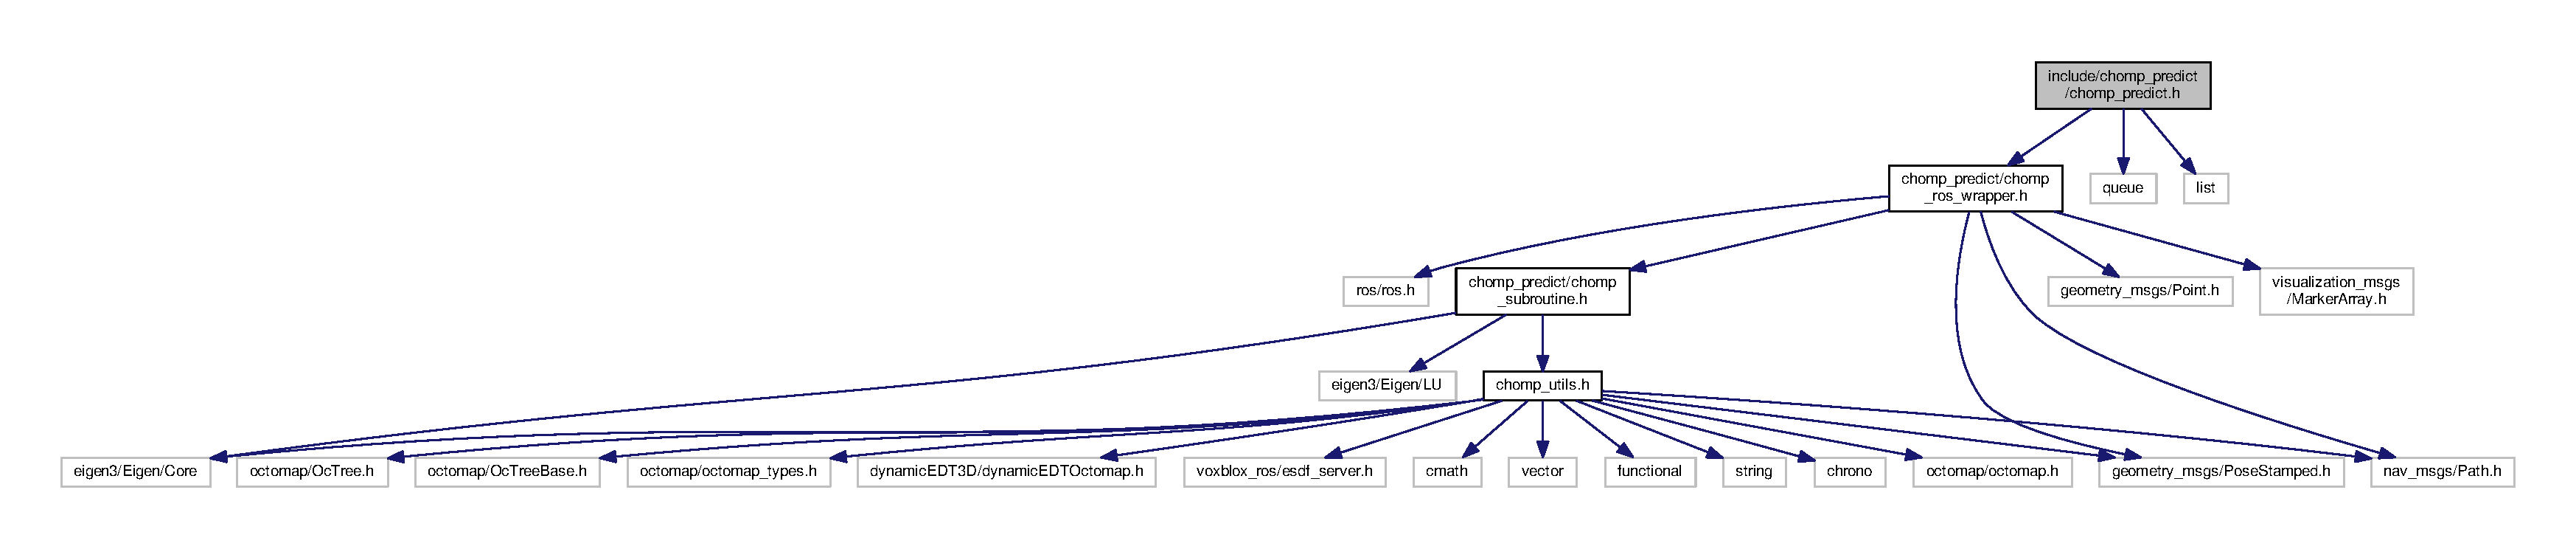
\includegraphics[width=350pt]{chomp__predict_8h__incl}
\end{center}
\end{figure}
This graph shows which files directly or indirectly include this file\+:\nopagebreak
\begin{figure}[H]
\begin{center}
\leavevmode
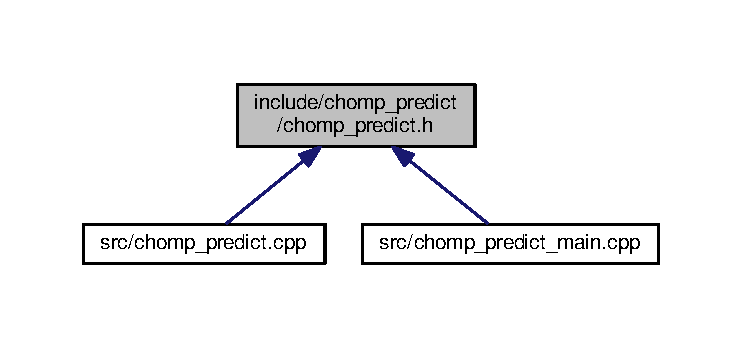
\includegraphics[width=350pt]{chomp__predict_8h__dep__incl}
\end{center}
\end{figure}
\subsection*{Classes}
\begin{DoxyCompactItemize}
\item 
struct \hyperlink{struct_c_h_o_m_p_1_1_predict_param}{C\+H\+O\+M\+P\+::\+Predict\+Param}
\item 
struct \hyperlink{struct_c_h_o_m_p_1_1_prediction_trajectory}{C\+H\+O\+M\+P\+::\+Prediction\+Trajectory}
\item 
class \hyperlink{class_c_h_o_m_p_1_1_chomp_forecaster}{C\+H\+O\+M\+P\+::\+Chomp\+Forecaster}
\end{DoxyCompactItemize}
\subsection*{Namespaces}
\begin{DoxyCompactItemize}
\item 
 \hyperlink{namespace_c_h_o_m_p}{C\+H\+O\+MP}
\begin{DoxyCompactList}\small\item\em This script solves the \hyperlink{namespace_c_h_o_m_p}{C\+H\+O\+MP} programming \+: 1/2 x\textquotesingle{}Ax + bx + f(x) This requires evaluation function for f(x) and grad\+\_\+f(x) as a function pointer and other parameter. \end{DoxyCompactList}\end{DoxyCompactItemize}
\subsection*{Variables}
\begin{DoxyCompactItemize}
\item 
const double \hyperlink{chomp__predict_8h_aa8bb66008e8cd0fb1c631a6e72d4feb8}{V\+\_\+\+M\+AX} = 1.\+5
\item 
const double \hyperlink{chomp__predict_8h_aa718bffd34f38cebf90848cd4f6ea3a6}{B\+I\+G\+\_\+T} = 1e+5
\item 
const double \hyperlink{chomp__predict_8h_addd6e24f6be79970a48f369b3b1e29d5}{R\+E\+A\+C\+H\+\_\+\+T\+OL} = 0.\+5
\end{DoxyCompactItemize}


\subsection{Variable Documentation}
\index{chomp\+\_\+predict.\+h@{chomp\+\_\+predict.\+h}!B\+I\+G\+\_\+T@{B\+I\+G\+\_\+T}}
\index{B\+I\+G\+\_\+T@{B\+I\+G\+\_\+T}!chomp\+\_\+predict.\+h@{chomp\+\_\+predict.\+h}}
\subsubsection[{\texorpdfstring{B\+I\+G\+\_\+T}{BIG_T}}]{\setlength{\rightskip}{0pt plus 5cm}const double B\+I\+G\+\_\+T = 1e+5}\hypertarget{chomp__predict_8h_aa718bffd34f38cebf90848cd4f6ea3a6}{}\label{chomp__predict_8h_aa718bffd34f38cebf90848cd4f6ea3a6}


Definition at line 7 of file chomp\+\_\+predict.\+h.

\index{chomp\+\_\+predict.\+h@{chomp\+\_\+predict.\+h}!R\+E\+A\+C\+H\+\_\+\+T\+OL@{R\+E\+A\+C\+H\+\_\+\+T\+OL}}
\index{R\+E\+A\+C\+H\+\_\+\+T\+OL@{R\+E\+A\+C\+H\+\_\+\+T\+OL}!chomp\+\_\+predict.\+h@{chomp\+\_\+predict.\+h}}
\subsubsection[{\texorpdfstring{R\+E\+A\+C\+H\+\_\+\+T\+OL}{REACH_TOL}}]{\setlength{\rightskip}{0pt plus 5cm}const double R\+E\+A\+C\+H\+\_\+\+T\+OL = 0.\+5}\hypertarget{chomp__predict_8h_addd6e24f6be79970a48f369b3b1e29d5}{}\label{chomp__predict_8h_addd6e24f6be79970a48f369b3b1e29d5}


Definition at line 8 of file chomp\+\_\+predict.\+h.

\index{chomp\+\_\+predict.\+h@{chomp\+\_\+predict.\+h}!V\+\_\+\+M\+AX@{V\+\_\+\+M\+AX}}
\index{V\+\_\+\+M\+AX@{V\+\_\+\+M\+AX}!chomp\+\_\+predict.\+h@{chomp\+\_\+predict.\+h}}
\subsubsection[{\texorpdfstring{V\+\_\+\+M\+AX}{V_MAX}}]{\setlength{\rightskip}{0pt plus 5cm}const double V\+\_\+\+M\+AX = 1.\+5}\hypertarget{chomp__predict_8h_aa8bb66008e8cd0fb1c631a6e72d4feb8}{}\label{chomp__predict_8h_aa8bb66008e8cd0fb1c631a6e72d4feb8}


Definition at line 6 of file chomp\+\_\+predict.\+h.


\hypertarget{chomp__ros__wrapper_8h}{}\section{include/chomp\+\_\+predict/chomp\+\_\+ros\+\_\+wrapper.h File Reference}
\label{chomp__ros__wrapper_8h}\index{include/chomp\+\_\+predict/chomp\+\_\+ros\+\_\+wrapper.\+h@{include/chomp\+\_\+predict/chomp\+\_\+ros\+\_\+wrapper.\+h}}
{\ttfamily \#include $<$ros/ros.\+h$>$}\\*
{\ttfamily \#include \char`\"{}chomp\+\_\+predict/chomp\+\_\+subroutine.\+h\char`\"{}}\\*
{\ttfamily \#include $<$geometry\+\_\+msgs/\+Pose\+Stamped.\+h$>$}\\*
{\ttfamily \#include $<$geometry\+\_\+msgs/\+Point.\+h$>$}\\*
{\ttfamily \#include $<$visualization\+\_\+msgs/\+Marker\+Array.\+h$>$}\\*
{\ttfamily \#include $<$nav\+\_\+msgs/\+Path.\+h$>$}\\*
Include dependency graph for chomp\+\_\+ros\+\_\+wrapper.\+h\+:\nopagebreak
\begin{figure}[H]
\begin{center}
\leavevmode
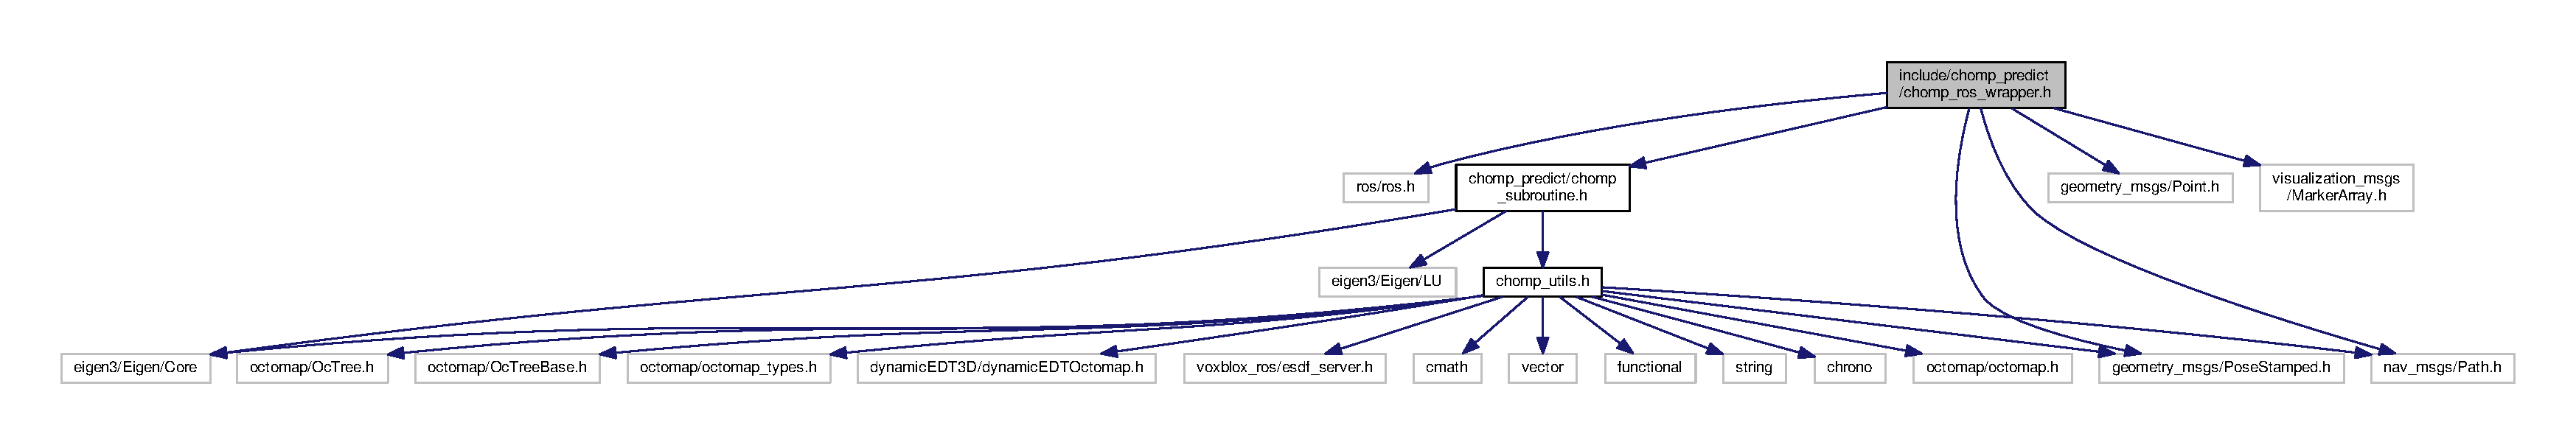
\includegraphics[width=350pt]{chomp__ros__wrapper_8h__incl}
\end{center}
\end{figure}
This graph shows which files directly or indirectly include this file\+:\nopagebreak
\begin{figure}[H]
\begin{center}
\leavevmode
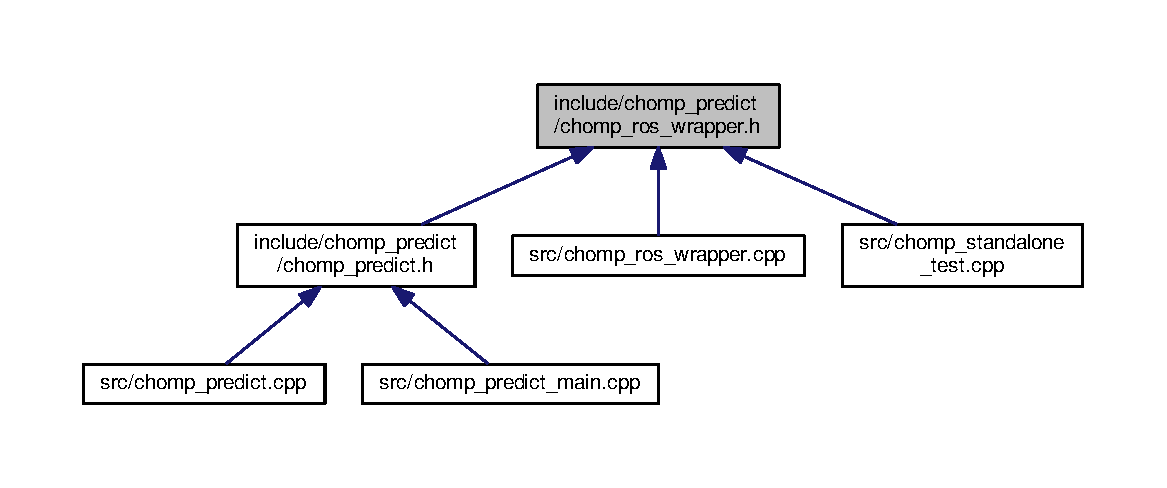
\includegraphics[width=350pt]{chomp__ros__wrapper_8h__dep__incl}
\end{center}
\end{figure}
\subsection*{Classes}
\begin{DoxyCompactItemize}
\item 
class \hyperlink{class_c_h_o_m_p_1_1_wrapper}{C\+H\+O\+M\+P\+::\+Wrapper}
\end{DoxyCompactItemize}
\subsection*{Namespaces}
\begin{DoxyCompactItemize}
\item 
 \hyperlink{namespace_c_h_o_m_p}{C\+H\+O\+MP}
\begin{DoxyCompactList}\small\item\em This script solves the \hyperlink{namespace_c_h_o_m_p}{C\+H\+O\+MP} programming \+: 1/2 x\textquotesingle{}Ax + bx + f(x) This requires evaluation function for f(x) and grad\+\_\+f(x) as a function pointer and other parameter. \end{DoxyCompactList}\end{DoxyCompactItemize}

\hypertarget{chomp__subroutine_8h}{}\section{include/chomp\+\_\+predict/chomp\+\_\+subroutine.h File Reference}
\label{chomp__subroutine_8h}\index{include/chomp\+\_\+predict/chomp\+\_\+subroutine.\+h@{include/chomp\+\_\+predict/chomp\+\_\+subroutine.\+h}}
{\ttfamily \#include $<$eigen3/\+Eigen/\+Core$>$}\\*
{\ttfamily \#include $<$eigen3/\+Eigen/\+LU$>$}\\*
{\ttfamily \#include \char`\"{}chomp\+\_\+utils.\+h\char`\"{}}\\*
Include dependency graph for chomp\+\_\+subroutine.\+h\+:\nopagebreak
\begin{figure}[H]
\begin{center}
\leavevmode
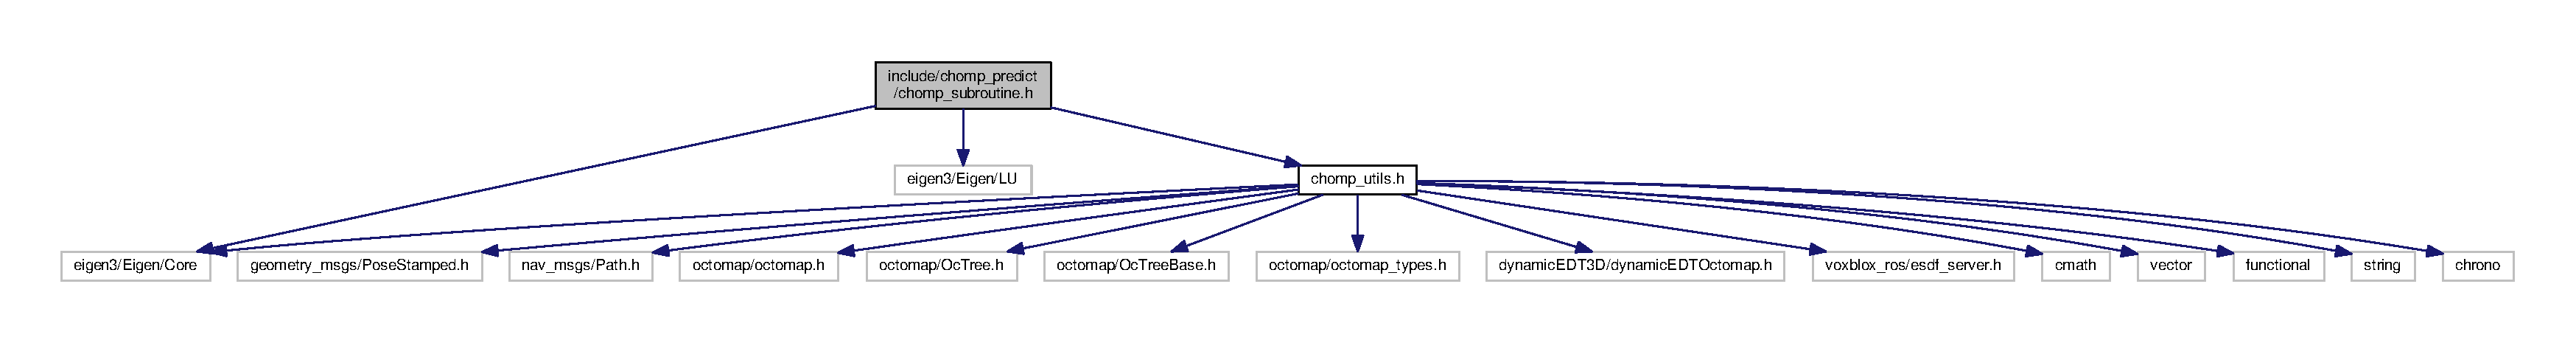
\includegraphics[width=350pt]{chomp__subroutine_8h__incl}
\end{center}
\end{figure}
This graph shows which files directly or indirectly include this file\+:\nopagebreak
\begin{figure}[H]
\begin{center}
\leavevmode
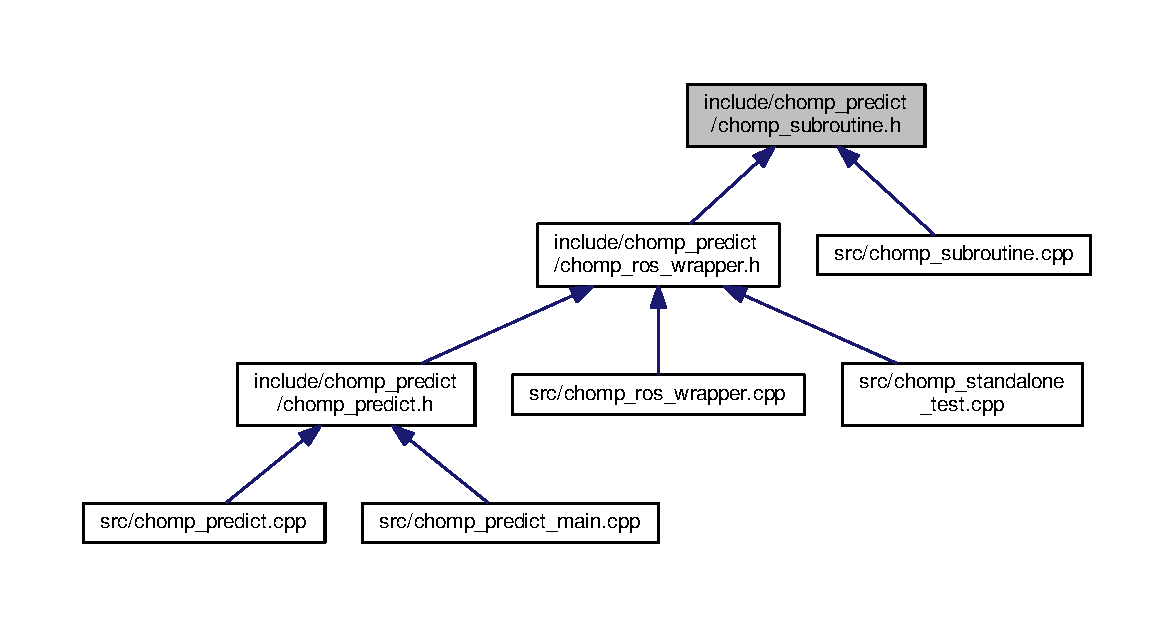
\includegraphics[width=350pt]{chomp__subroutine_8h__dep__incl}
\end{center}
\end{figure}
\subsection*{Classes}
\begin{DoxyCompactItemize}
\item 
class \hyperlink{classshaping__functor}{shaping\+\_\+functor}
\begin{DoxyCompactList}\small\item\em Functor for shaping function from distance\+\_\+raw. \end{DoxyCompactList}\item 
class \hyperlink{classshaping__functor__grad}{shaping\+\_\+functor\+\_\+grad}
\item 
struct \hyperlink{struct_c_h_o_m_p_1_1_cost_param}{C\+H\+O\+M\+P\+::\+Cost\+Param}
\item 
struct \hyperlink{struct_c_h_o_m_p_1_1_optim_param}{C\+H\+O\+M\+P\+::\+Optim\+Param}
\item 
struct \hyperlink{struct_c_h_o_m_p_1_1_optim_info}{C\+H\+O\+M\+P\+::\+Optim\+Info}
\item 
struct \hyperlink{struct_c_h_o_m_p_1_1_optim_result}{C\+H\+O\+M\+P\+::\+Optim\+Result}
\item 
struct \hyperlink{struct_c_h_o_m_p_1_1_optim_grad}{C\+H\+O\+M\+P\+::\+Optim\+Grad}
\begin{DoxyCompactList}\small\item\em gradient containing prior and nonlinear together \end{DoxyCompactList}\item 
class \hyperlink{class_c_h_o_m_p_1_1_solver}{C\+H\+O\+M\+P\+::\+Solver}
\end{DoxyCompactItemize}
\subsection*{Namespaces}
\begin{DoxyCompactItemize}
\item 
 \hyperlink{namespace_c_h_o_m_p}{C\+H\+O\+MP}
\begin{DoxyCompactList}\small\item\em This script solves the \hyperlink{namespace_c_h_o_m_p}{C\+H\+O\+MP} programming \+: 1/2 x\textquotesingle{}Ax + bx + f(x) This requires evaluation function for f(x) and grad\+\_\+f(x) as a function pointer and other parameter. \end{DoxyCompactList}\end{DoxyCompactItemize}
\subsection*{Macros}
\begin{DoxyCompactItemize}
\item 
\#define \hyperlink{chomp__subroutine_8h_af8236cba31aaebf449b6e72a1fd0b7e9}{D\+I\+M\+\_\+\+E\+X\+C\+E\+P\+T\+I\+ON}~0;
\end{DoxyCompactItemize}


\subsection{Macro Definition Documentation}
\index{chomp\+\_\+subroutine.\+h@{chomp\+\_\+subroutine.\+h}!D\+I\+M\+\_\+\+E\+X\+C\+E\+P\+T\+I\+ON@{D\+I\+M\+\_\+\+E\+X\+C\+E\+P\+T\+I\+ON}}
\index{D\+I\+M\+\_\+\+E\+X\+C\+E\+P\+T\+I\+ON@{D\+I\+M\+\_\+\+E\+X\+C\+E\+P\+T\+I\+ON}!chomp\+\_\+subroutine.\+h@{chomp\+\_\+subroutine.\+h}}
\subsubsection[{\texorpdfstring{D\+I\+M\+\_\+\+E\+X\+C\+E\+P\+T\+I\+ON}{DIM_EXCEPTION}}]{\setlength{\rightskip}{0pt plus 5cm}\#define D\+I\+M\+\_\+\+E\+X\+C\+E\+P\+T\+I\+ON~0;}\hypertarget{chomp__subroutine_8h_af8236cba31aaebf449b6e72a1fd0b7e9}{}\label{chomp__subroutine_8h_af8236cba31aaebf449b6e72a1fd0b7e9}


Definition at line 6 of file chomp\+\_\+subroutine.\+h.


\hypertarget{chomp__utils_8h}{}\section{include/chomp\+\_\+utils.h File Reference}
\label{chomp__utils_8h}\index{include/chomp\+\_\+utils.\+h@{include/chomp\+\_\+utils.\+h}}
{\ttfamily \#include $<$eigen3/\+Eigen/\+Core$>$}\\*
{\ttfamily \#include $<$geometry\+\_\+msgs/\+Pose\+Stamped.\+h$>$}\\*
{\ttfamily \#include $<$nav\+\_\+msgs/\+Path.\+h$>$}\\*
{\ttfamily \#include $<$octomap/octomap.\+h$>$}\\*
{\ttfamily \#include $<$octomap/\+Oc\+Tree.\+h$>$}\\*
{\ttfamily \#include $<$octomap/\+Oc\+Tree\+Base.\+h$>$}\\*
{\ttfamily \#include $<$octomap/octomap\+\_\+types.\+h$>$}\\*
{\ttfamily \#include $<$dynamic\+E\+D\+T3\+D/dynamic\+E\+D\+T\+Octomap.\+h$>$}\\*
{\ttfamily \#include $<$voxblox\+\_\+ros/esdf\+\_\+server.\+h$>$}\\*
{\ttfamily \#include $<$cmath$>$}\\*
{\ttfamily \#include $<$vector$>$}\\*
{\ttfamily \#include $<$functional$>$}\\*
{\ttfamily \#include $<$string$>$}\\*
{\ttfamily \#include $<$chrono$>$}\\*
Include dependency graph for chomp\+\_\+utils.\+h\+:\nopagebreak
\begin{figure}[H]
\begin{center}
\leavevmode
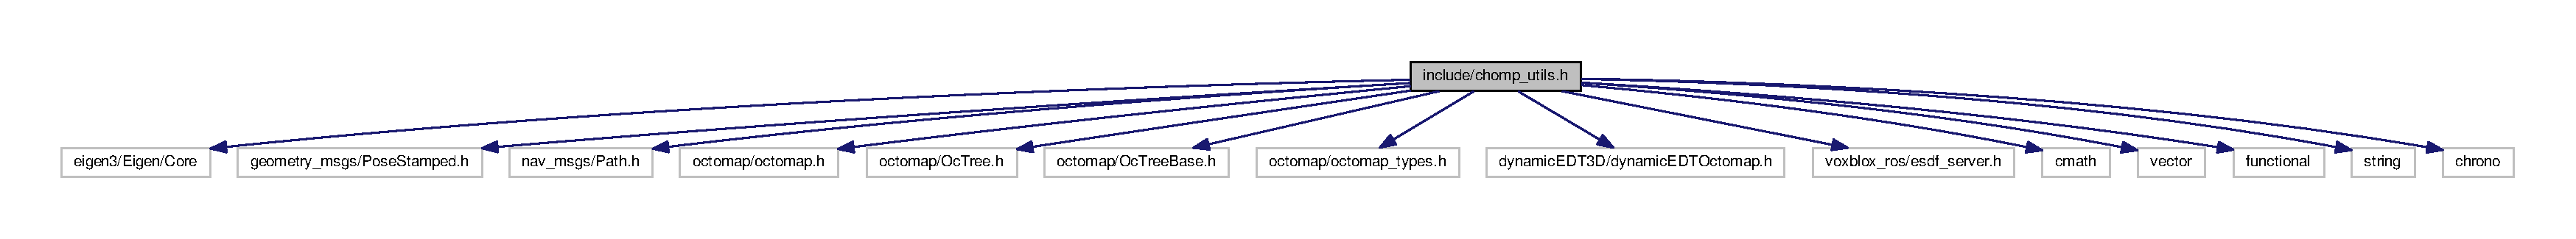
\includegraphics[width=350pt]{chomp__utils_8h__incl}
\end{center}
\end{figure}
This graph shows which files directly or indirectly include this file\+:\nopagebreak
\begin{figure}[H]
\begin{center}
\leavevmode
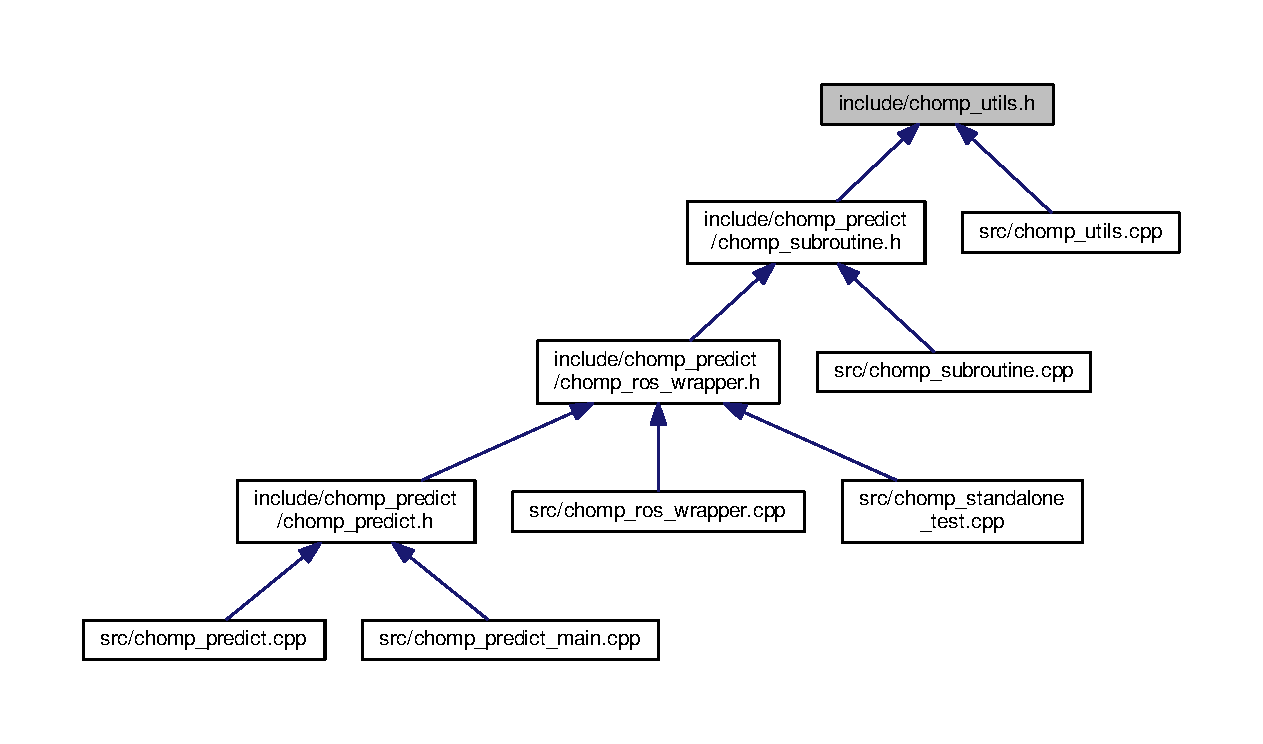
\includegraphics[width=350pt]{chomp__utils_8h__dep__incl}
\end{center}
\end{figure}
\subsection*{Classes}
\begin{DoxyCompactItemize}
\item 
struct \hyperlink{struct_linear_model}{Linear\+Model}
\end{DoxyCompactItemize}
\subsection*{Functions}
\begin{DoxyCompactItemize}
\item 
\hyperlink{struct_linear_model}{Linear\+Model} \hyperlink{chomp__utils_8h_a01e43aa8fc67413d2ad3ee7e840bb66e}{linear\+\_\+regression} (const Eigen\+::\+Vector\+Xd \&ts, const Eigen\+::\+Vector\+Xd \&xs)
\item 
double \hyperlink{chomp__utils_8h_ada013a3d8e591b8122e95dfab24eace1}{model\+\_\+eval} (const \hyperlink{struct_linear_model}{Linear\+Model} \&model, double t)
\item 
void \hyperlink{chomp__utils_8h_a18dbbf76a331741ef17e17e5550585df}{path2vec} (const nav\+\_\+msgs\+::\+Path \&path, std\+::vector$<$ double $>$ \&xs, std\+::vector$<$ double $>$ \&ys, std\+::vector$<$ double $>$ \&zs)
\item 
void \hyperlink{chomp__utils_8h_ad9f1c9686aec6d42004aee2c109bea82}{vec2path} (std\+::vector$<$ double $>$ \&xs, std\+::vector$<$ double $>$ \&ys, std\+::vector$<$ double $>$ \&zs, nav\+\_\+msgs\+::\+Path \&path)
\item 
Eigen\+::\+Vector\+Xd \hyperlink{chomp__utils_8h_a375713c39c1bc5b4ba9357af46a3082e}{get\+\_\+time\+\_\+stamps\+\_\+from\+\_\+nav\+\_\+path} (const nav\+\_\+msgs\+::\+Path \&path)
\item 
double \hyperlink{chomp__utils_8h_a0fa75528fdd2f1dc601c4d4e7da6a6b0}{interpolate} (Eigen\+::\+Vector\+Xd \&x\+Data, Eigen\+::\+Vector\+Xd \&y\+Data, double x, bool extrapolate)
\end{DoxyCompactItemize}


\subsection{Function Documentation}
\index{chomp\+\_\+utils.\+h@{chomp\+\_\+utils.\+h}!get\+\_\+time\+\_\+stamps\+\_\+from\+\_\+nav\+\_\+path@{get\+\_\+time\+\_\+stamps\+\_\+from\+\_\+nav\+\_\+path}}
\index{get\+\_\+time\+\_\+stamps\+\_\+from\+\_\+nav\+\_\+path@{get\+\_\+time\+\_\+stamps\+\_\+from\+\_\+nav\+\_\+path}!chomp\+\_\+utils.\+h@{chomp\+\_\+utils.\+h}}
\subsubsection[{\texorpdfstring{get\+\_\+time\+\_\+stamps\+\_\+from\+\_\+nav\+\_\+path(const nav\+\_\+msgs\+::\+Path \&path)}{get_time_stamps_from_nav_path(const nav_msgs::Path &path)}}]{\setlength{\rightskip}{0pt plus 5cm}Eigen\+::\+Vector\+Xd get\+\_\+time\+\_\+stamps\+\_\+from\+\_\+nav\+\_\+path (
\begin{DoxyParamCaption}
\item[{const nav\+\_\+msgs\+::\+Path \&}]{path}
\end{DoxyParamCaption}
)}\hypertarget{chomp__utils_8h_a375713c39c1bc5b4ba9357af46a3082e}{}\label{chomp__utils_8h_a375713c39c1bc5b4ba9357af46a3082e}


Definition at line 55 of file chomp\+\_\+utils.\+cpp.

\index{chomp\+\_\+utils.\+h@{chomp\+\_\+utils.\+h}!interpolate@{interpolate}}
\index{interpolate@{interpolate}!chomp\+\_\+utils.\+h@{chomp\+\_\+utils.\+h}}
\subsubsection[{\texorpdfstring{interpolate(\+Eigen\+::\+Vector\+Xd \&x\+Data, Eigen\+::\+Vector\+Xd \&y\+Data, double x, bool extrapolate)}{interpolate(Eigen::VectorXd &xData, Eigen::VectorXd &yData, double x, bool extrapolate)}}]{\setlength{\rightskip}{0pt plus 5cm}double interpolate (
\begin{DoxyParamCaption}
\item[{Eigen\+::\+Vector\+Xd \&}]{x\+Data, }
\item[{Eigen\+::\+Vector\+Xd \&}]{y\+Data, }
\item[{double}]{x, }
\item[{bool}]{extrapolate}
\end{DoxyParamCaption}
)}\hypertarget{chomp__utils_8h_a0fa75528fdd2f1dc601c4d4e7da6a6b0}{}\label{chomp__utils_8h_a0fa75528fdd2f1dc601c4d4e7da6a6b0}


Definition at line 66 of file chomp\+\_\+utils.\+cpp.



Here is the caller graph for this function\+:
\nopagebreak
\begin{figure}[H]
\begin{center}
\leavevmode
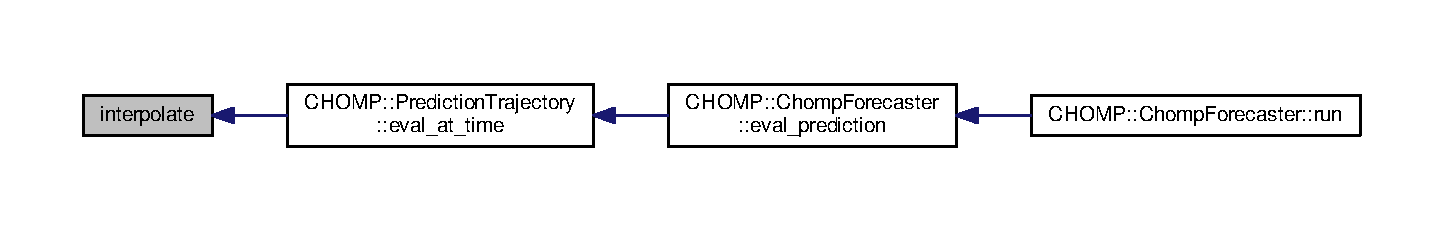
\includegraphics[width=350pt]{chomp__utils_8h_a0fa75528fdd2f1dc601c4d4e7da6a6b0_icgraph}
\end{center}
\end{figure}


\index{chomp\+\_\+utils.\+h@{chomp\+\_\+utils.\+h}!linear\+\_\+regression@{linear\+\_\+regression}}
\index{linear\+\_\+regression@{linear\+\_\+regression}!chomp\+\_\+utils.\+h@{chomp\+\_\+utils.\+h}}
\subsubsection[{\texorpdfstring{linear\+\_\+regression(const Eigen\+::\+Vector\+Xd \&ts, const Eigen\+::\+Vector\+Xd \&xs)}{linear_regression(const Eigen::VectorXd &ts, const Eigen::VectorXd &xs)}}]{\setlength{\rightskip}{0pt plus 5cm}{\bf Linear\+Model} linear\+\_\+regression (
\begin{DoxyParamCaption}
\item[{const Eigen\+::\+Vector\+Xd \&}]{ts, }
\item[{const Eigen\+::\+Vector\+Xd \&}]{xs}
\end{DoxyParamCaption}
)}\hypertarget{chomp__utils_8h_a01e43aa8fc67413d2ad3ee7e840bb66e}{}\label{chomp__utils_8h_a01e43aa8fc67413d2ad3ee7e840bb66e}


Definition at line 3 of file chomp\+\_\+utils.\+cpp.



Here is the caller graph for this function\+:
\nopagebreak
\begin{figure}[H]
\begin{center}
\leavevmode
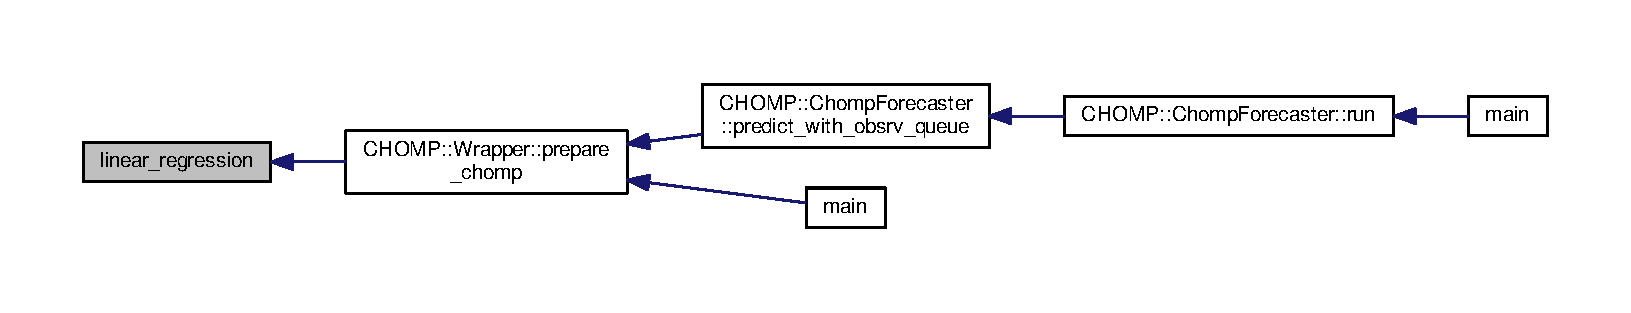
\includegraphics[width=350pt]{chomp__utils_8h_a01e43aa8fc67413d2ad3ee7e840bb66e_icgraph}
\end{center}
\end{figure}


\index{chomp\+\_\+utils.\+h@{chomp\+\_\+utils.\+h}!model\+\_\+eval@{model\+\_\+eval}}
\index{model\+\_\+eval@{model\+\_\+eval}!chomp\+\_\+utils.\+h@{chomp\+\_\+utils.\+h}}
\subsubsection[{\texorpdfstring{model\+\_\+eval(const Linear\+Model \&model, double t)}{model_eval(const LinearModel &model, double t)}}]{\setlength{\rightskip}{0pt plus 5cm}double model\+\_\+eval (
\begin{DoxyParamCaption}
\item[{const {\bf Linear\+Model} \&}]{model, }
\item[{double}]{t}
\end{DoxyParamCaption}
)}\hypertarget{chomp__utils_8h_ada013a3d8e591b8122e95dfab24eace1}{}\label{chomp__utils_8h_ada013a3d8e591b8122e95dfab24eace1}


Definition at line 20 of file chomp\+\_\+utils.\+cpp.



Here is the caller graph for this function\+:
\nopagebreak
\begin{figure}[H]
\begin{center}
\leavevmode
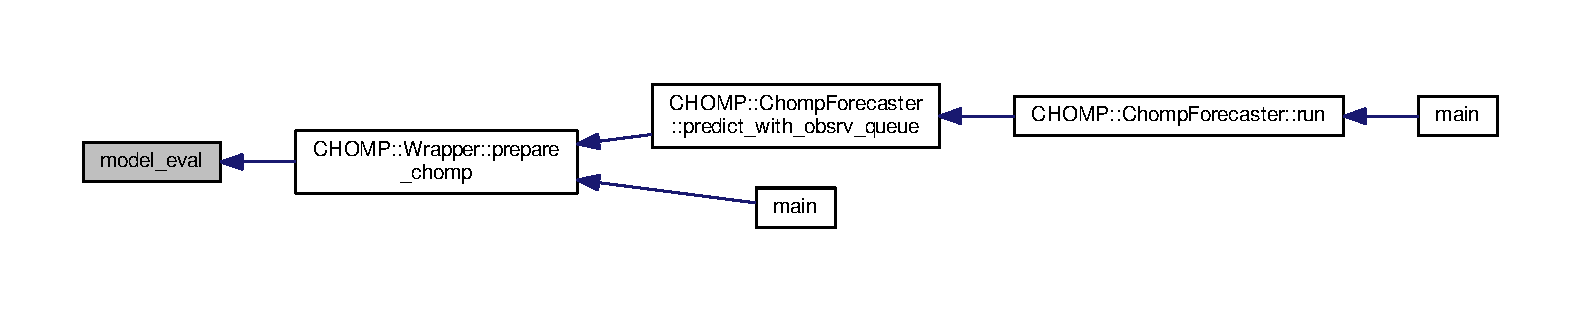
\includegraphics[width=350pt]{chomp__utils_8h_ada013a3d8e591b8122e95dfab24eace1_icgraph}
\end{center}
\end{figure}


\index{chomp\+\_\+utils.\+h@{chomp\+\_\+utils.\+h}!path2vec@{path2vec}}
\index{path2vec@{path2vec}!chomp\+\_\+utils.\+h@{chomp\+\_\+utils.\+h}}
\subsubsection[{\texorpdfstring{path2vec(const nav\+\_\+msgs\+::\+Path \&path, std\+::vector$<$ double $>$ \&xs, std\+::vector$<$ double $>$ \&ys, std\+::vector$<$ double $>$ \&zs)}{path2vec(const nav_msgs::Path &path, std::vector< double > &xs, std::vector< double > &ys, std::vector< double > &zs)}}]{\setlength{\rightskip}{0pt plus 5cm}void path2vec (
\begin{DoxyParamCaption}
\item[{const nav\+\_\+msgs\+::\+Path \&}]{path, }
\item[{std\+::vector$<$ double $>$ \&}]{xs, }
\item[{std\+::vector$<$ double $>$ \&}]{ys, }
\item[{std\+::vector$<$ double $>$ \&}]{zs}
\end{DoxyParamCaption}
)}\hypertarget{chomp__utils_8h_a18dbbf76a331741ef17e17e5550585df}{}\label{chomp__utils_8h_a18dbbf76a331741ef17e17e5550585df}


Definition at line 40 of file chomp\+\_\+utils.\+cpp.



Here is the caller graph for this function\+:
\nopagebreak
\begin{figure}[H]
\begin{center}
\leavevmode
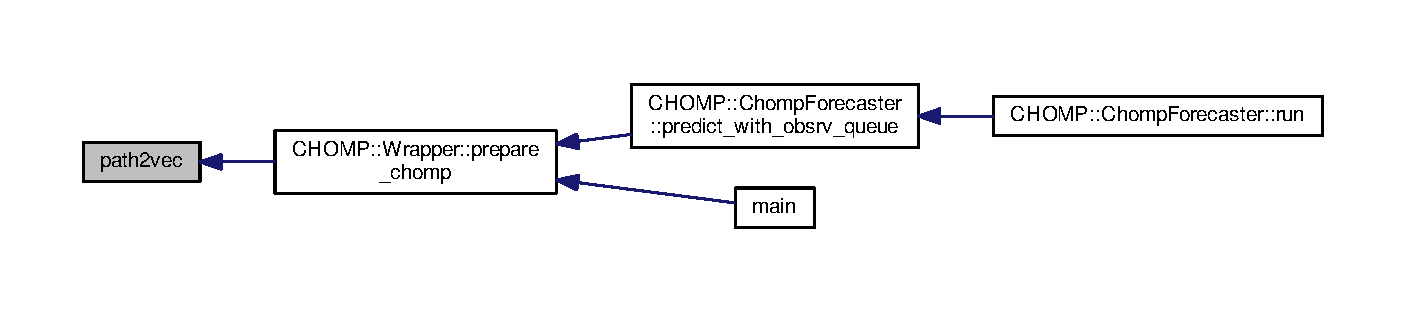
\includegraphics[width=350pt]{chomp__utils_8h_a18dbbf76a331741ef17e17e5550585df_icgraph}
\end{center}
\end{figure}


\index{chomp\+\_\+utils.\+h@{chomp\+\_\+utils.\+h}!vec2path@{vec2path}}
\index{vec2path@{vec2path}!chomp\+\_\+utils.\+h@{chomp\+\_\+utils.\+h}}
\subsubsection[{\texorpdfstring{vec2path(std\+::vector$<$ double $>$ \&xs, std\+::vector$<$ double $>$ \&ys, std\+::vector$<$ double $>$ \&zs, nav\+\_\+msgs\+::\+Path \&path)}{vec2path(std::vector< double > &xs, std::vector< double > &ys, std::vector< double > &zs, nav_msgs::Path &path)}}]{\setlength{\rightskip}{0pt plus 5cm}void vec2path (
\begin{DoxyParamCaption}
\item[{std\+::vector$<$ double $>$ \&}]{xs, }
\item[{std\+::vector$<$ double $>$ \&}]{ys, }
\item[{std\+::vector$<$ double $>$ \&}]{zs, }
\item[{nav\+\_\+msgs\+::\+Path \&}]{path}
\end{DoxyParamCaption}
)}\hypertarget{chomp__utils_8h_ad9f1c9686aec6d42004aee2c109bea82}{}\label{chomp__utils_8h_ad9f1c9686aec6d42004aee2c109bea82}


Definition at line 25 of file chomp\+\_\+utils.\+cpp.


\hypertarget{_r_e_a_d_m_e_8md}{}\section{R\+E\+A\+D\+M\+E.\+md File Reference}
\label{_r_e_a_d_m_e_8md}\index{R\+E\+A\+D\+M\+E.\+md@{R\+E\+A\+D\+M\+E.\+md}}

\hypertarget{chomp__predict_8cpp}{}\section{src/chomp\+\_\+predict.cpp File Reference}
\label{chomp__predict_8cpp}\index{src/chomp\+\_\+predict.\+cpp@{src/chomp\+\_\+predict.\+cpp}}
{\ttfamily \#include $<$chomp\+\_\+predict/chomp\+\_\+predict.\+h$>$}\\*
Include dependency graph for chomp\+\_\+predict.\+cpp\+:\nopagebreak
\begin{figure}[H]
\begin{center}
\leavevmode
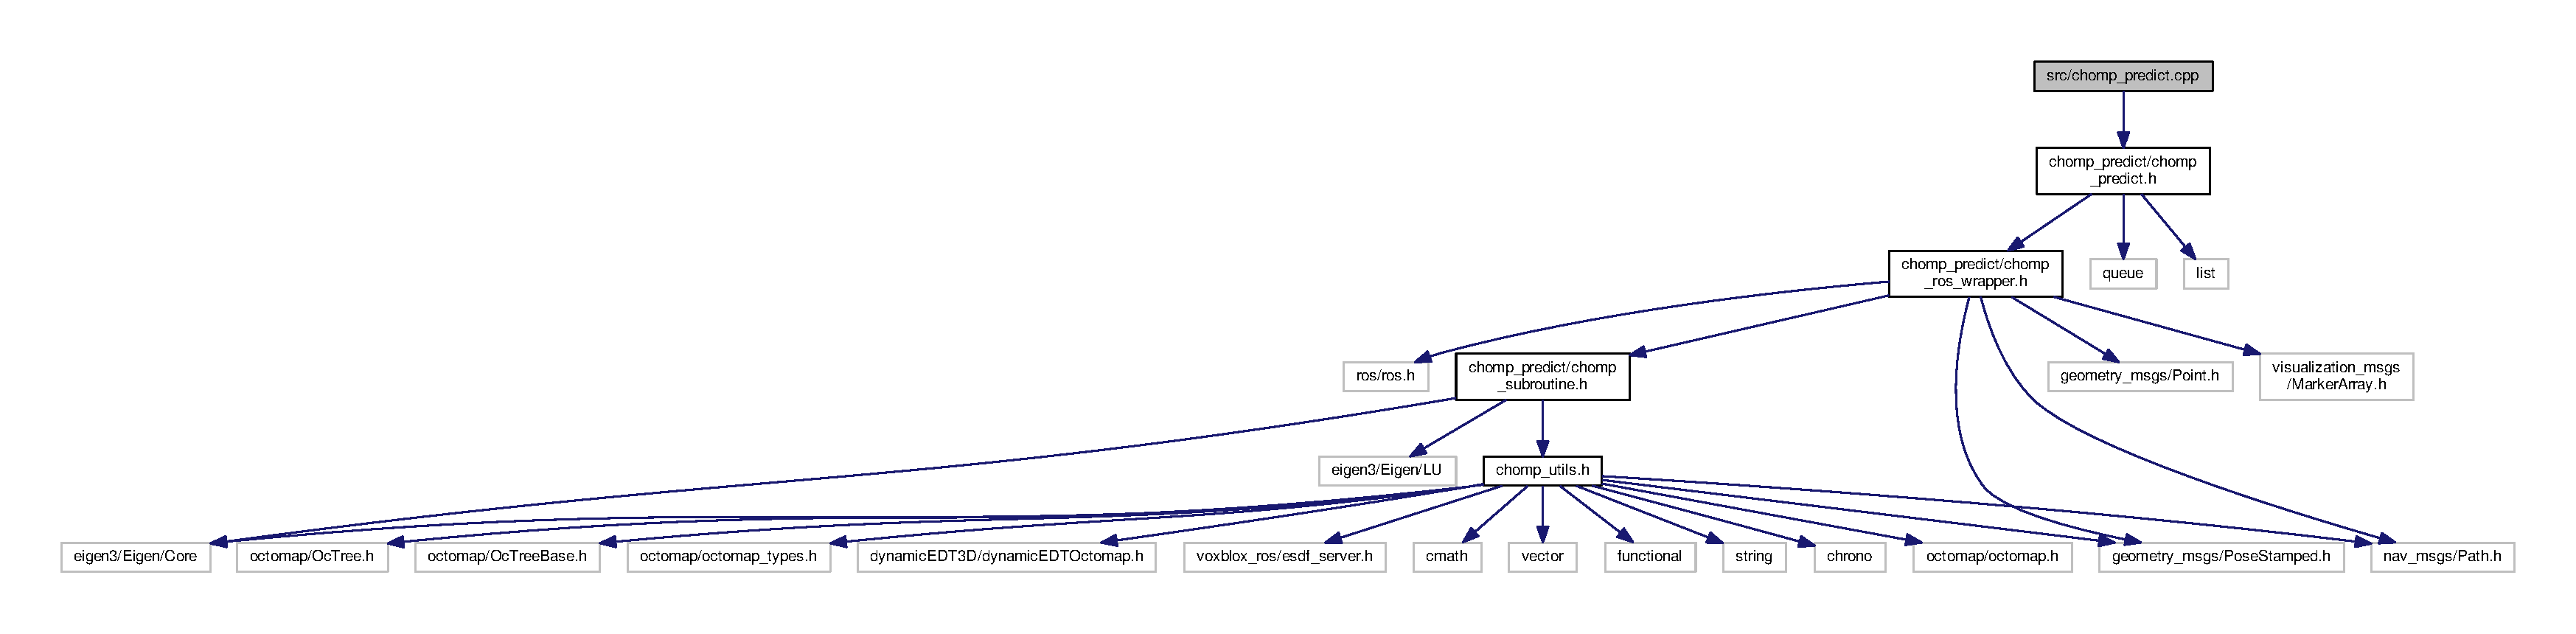
\includegraphics[width=350pt]{chomp__predict_8cpp__incl}
\end{center}
\end{figure}

\hypertarget{chomp__predict__main_8cpp}{}\section{src/chomp\+\_\+predict\+\_\+main.cpp File Reference}
\label{chomp__predict__main_8cpp}\index{src/chomp\+\_\+predict\+\_\+main.\+cpp@{src/chomp\+\_\+predict\+\_\+main.\+cpp}}
{\ttfamily \#include $<$chomp\+\_\+predict/chomp\+\_\+predict.\+h$>$}\\*
Include dependency graph for chomp\+\_\+predict\+\_\+main.\+cpp\+:
\nopagebreak
\begin{figure}[H]
\begin{center}
\leavevmode
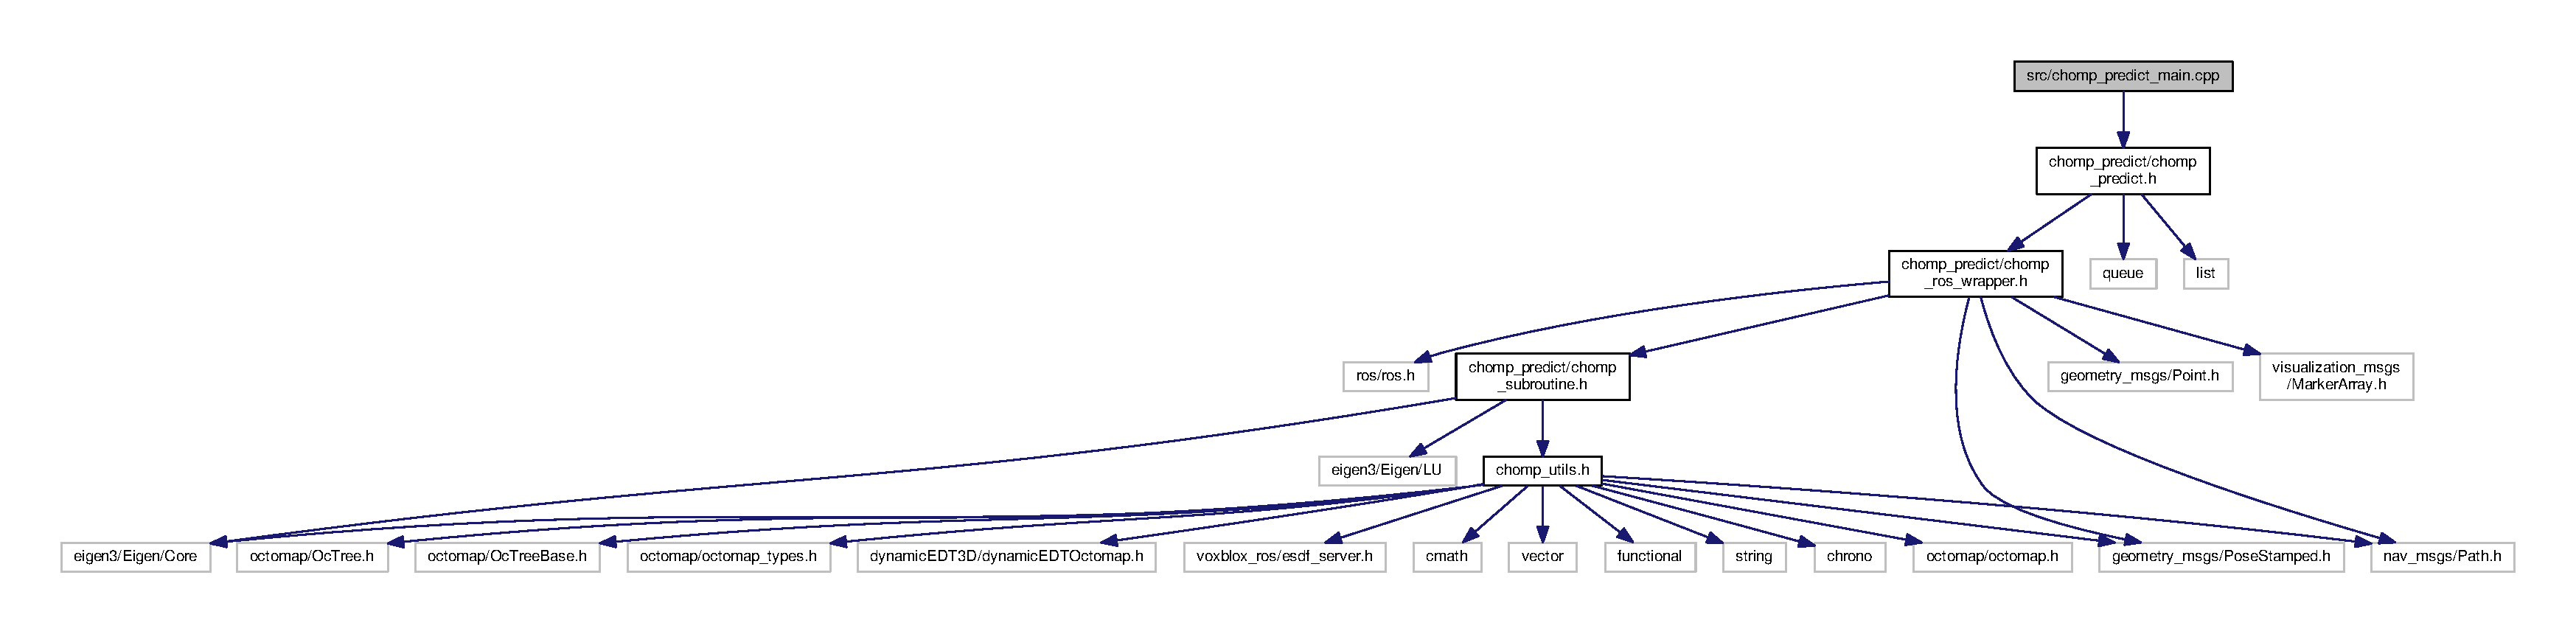
\includegraphics[width=350pt]{chomp__predict__main_8cpp__incl}
\end{center}
\end{figure}
\subsection*{Functions}
\begin{DoxyCompactItemize}
\item 
int \hyperlink{chomp__predict__main_8cpp_a0ddf1224851353fc92bfbff6f499fa97}{main} (int argc, char $\ast$argv\mbox{[}$\,$\mbox{]})
\end{DoxyCompactItemize}


\subsection{Function Documentation}
\index{chomp\+\_\+predict\+\_\+main.\+cpp@{chomp\+\_\+predict\+\_\+main.\+cpp}!main@{main}}
\index{main@{main}!chomp\+\_\+predict\+\_\+main.\+cpp@{chomp\+\_\+predict\+\_\+main.\+cpp}}
\subsubsection[{\texorpdfstring{main(int argc, char $\ast$argv[])}{main(int argc, char *argv[])}}]{\setlength{\rightskip}{0pt plus 5cm}int main (
\begin{DoxyParamCaption}
\item[{int}]{argc, }
\item[{char $\ast$}]{argv\mbox{[}$\,$\mbox{]}}
\end{DoxyParamCaption}
)}\hypertarget{chomp__predict__main_8cpp_a0ddf1224851353fc92bfbff6f499fa97}{}\label{chomp__predict__main_8cpp_a0ddf1224851353fc92bfbff6f499fa97}


Definition at line 3 of file chomp\+\_\+predict\+\_\+main.\+cpp.


\hypertarget{chomp__ros__wrapper_8cpp}{}\section{src/chomp\+\_\+ros\+\_\+wrapper.cpp File Reference}
\label{chomp__ros__wrapper_8cpp}\index{src/chomp\+\_\+ros\+\_\+wrapper.\+cpp@{src/chomp\+\_\+ros\+\_\+wrapper.\+cpp}}
{\ttfamily \#include \char`\"{}chomp\+\_\+predict/chomp\+\_\+ros\+\_\+wrapper.\+h\char`\"{}}\\*
Include dependency graph for chomp\+\_\+ros\+\_\+wrapper.\+cpp\+:\nopagebreak
\begin{figure}[H]
\begin{center}
\leavevmode
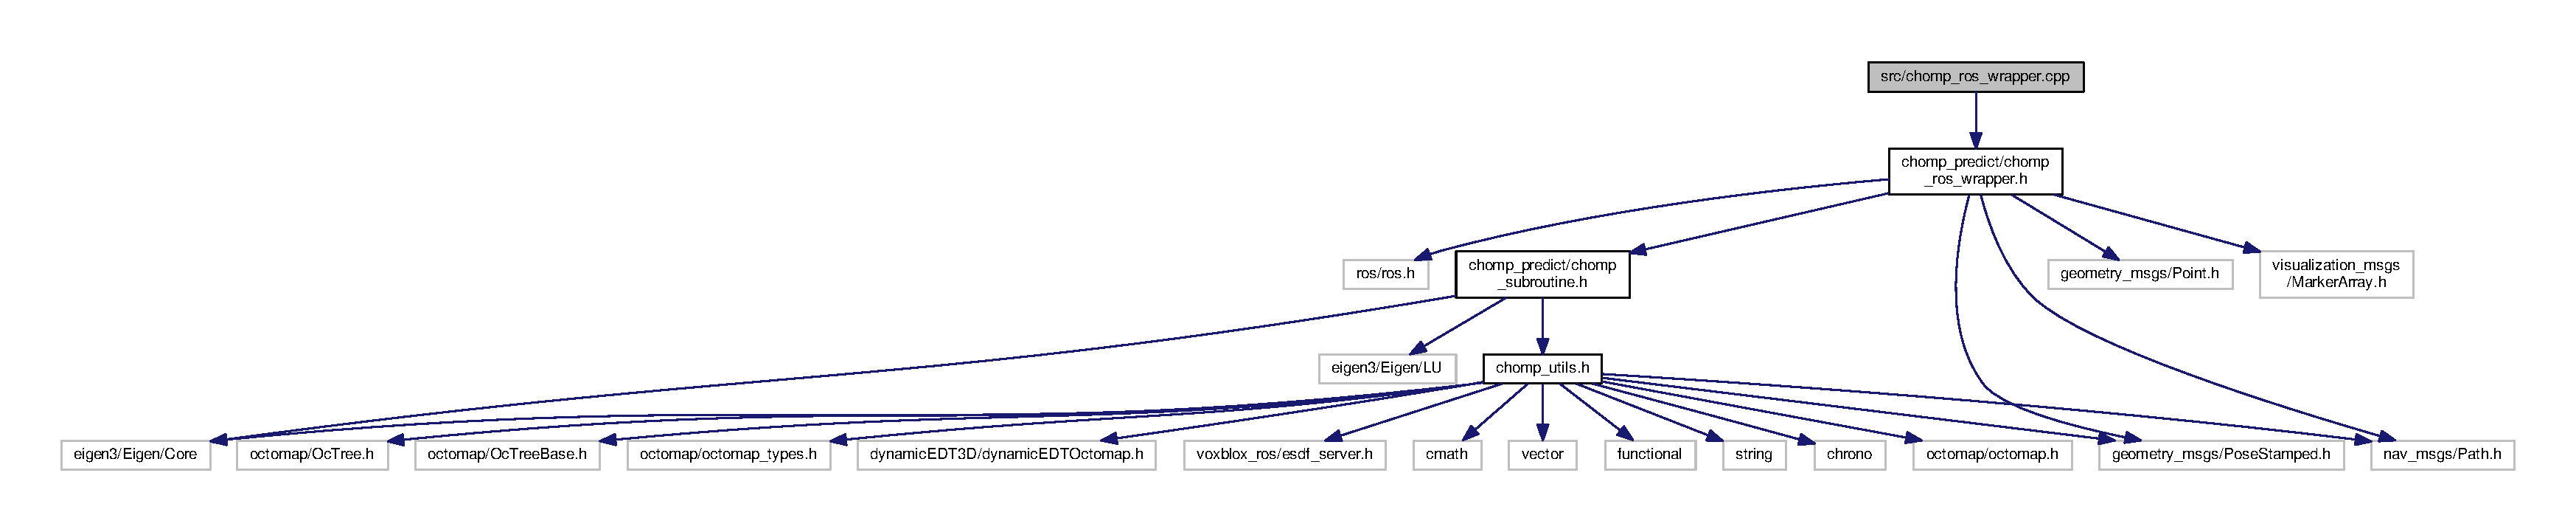
\includegraphics[width=350pt]{chomp__ros__wrapper_8cpp__incl}
\end{center}
\end{figure}

\hypertarget{chomp__standalone__test_8cpp}{}\section{src/chomp\+\_\+standalone\+\_\+test.cpp File Reference}
\label{chomp__standalone__test_8cpp}\index{src/chomp\+\_\+standalone\+\_\+test.\+cpp@{src/chomp\+\_\+standalone\+\_\+test.\+cpp}}
{\ttfamily \#include \char`\"{}chomp\+\_\+predict/chomp\+\_\+ros\+\_\+wrapper.\+h\char`\"{}}\\*
Include dependency graph for chomp\+\_\+standalone\+\_\+test.\+cpp\+:
\nopagebreak
\begin{figure}[H]
\begin{center}
\leavevmode
\includegraphics[width=350pt]{chomp__standalone__test_8cpp__incl}
\end{center}
\end{figure}
\subsection*{Functions}
\begin{DoxyCompactItemize}
\item 
int \hyperlink{chomp__standalone__test_8cpp_a0ddf1224851353fc92bfbff6f499fa97}{main} (int argc, char $\ast$argv\mbox{[}$\,$\mbox{]})
\end{DoxyCompactItemize}


\subsection{Function Documentation}
\index{chomp\+\_\+standalone\+\_\+test.\+cpp@{chomp\+\_\+standalone\+\_\+test.\+cpp}!main@{main}}
\index{main@{main}!chomp\+\_\+standalone\+\_\+test.\+cpp@{chomp\+\_\+standalone\+\_\+test.\+cpp}}
\subsubsection[{\texorpdfstring{main(int argc, char $\ast$argv[])}{main(int argc, char *argv[])}}]{\setlength{\rightskip}{0pt plus 5cm}int main (
\begin{DoxyParamCaption}
\item[{int}]{argc, }
\item[{char $\ast$}]{argv\mbox{[}$\,$\mbox{]}}
\end{DoxyParamCaption}
)}\hypertarget{chomp__standalone__test_8cpp_a0ddf1224851353fc92bfbff6f499fa97}{}\label{chomp__standalone__test_8cpp_a0ddf1224851353fc92bfbff6f499fa97}


Definition at line 6 of file chomp\+\_\+standalone\+\_\+test.\+cpp.



Here is the call graph for this function\+:
\nopagebreak
\begin{figure}[H]
\begin{center}
\leavevmode
\includegraphics[width=350pt]{chomp__standalone__test_8cpp_a0ddf1224851353fc92bfbff6f499fa97_cgraph}
\end{center}
\end{figure}



\hypertarget{chomp__subroutine_8cpp}{}\section{src/chomp\+\_\+subroutine.cpp File Reference}
\label{chomp__subroutine_8cpp}\index{src/chomp\+\_\+subroutine.\+cpp@{src/chomp\+\_\+subroutine.\+cpp}}
{\ttfamily \#include \char`\"{}chomp\+\_\+predict/chomp\+\_\+subroutine.\+h\char`\"{}}\\*
Include dependency graph for chomp\+\_\+subroutine.\+cpp\+:\nopagebreak
\begin{figure}[H]
\begin{center}
\leavevmode
\includegraphics[width=350pt]{chomp__subroutine_8cpp__incl}
\end{center}
\end{figure}

\hypertarget{chomp__utils_8cpp}{}\section{src/chomp\+\_\+utils.cpp File Reference}
\label{chomp__utils_8cpp}\index{src/chomp\+\_\+utils.\+cpp@{src/chomp\+\_\+utils.\+cpp}}
{\ttfamily \#include \char`\"{}chomp\+\_\+utils.\+h\char`\"{}}\\*
Include dependency graph for chomp\+\_\+utils.\+cpp\+:
\nopagebreak
\begin{figure}[H]
\begin{center}
\leavevmode
\includegraphics[width=350pt]{chomp__utils_8cpp__incl}
\end{center}
\end{figure}
\subsection*{Functions}
\begin{DoxyCompactItemize}
\item 
\hyperlink{struct_linear_model}{Linear\+Model} \hyperlink{chomp__utils_8cpp_a01e43aa8fc67413d2ad3ee7e840bb66e}{linear\+\_\+regression} (const Eigen\+::\+Vector\+Xd \&ts, const Eigen\+::\+Vector\+Xd \&xs)
\item 
double \hyperlink{chomp__utils_8cpp_ada013a3d8e591b8122e95dfab24eace1}{model\+\_\+eval} (const \hyperlink{struct_linear_model}{Linear\+Model} \&model, double t)
\item 
void \hyperlink{chomp__utils_8cpp_ad9f1c9686aec6d42004aee2c109bea82}{vec2path} (std\+::vector$<$ double $>$ \&xs, std\+::vector$<$ double $>$ \&ys, std\+::vector$<$ double $>$ \&zs, nav\+\_\+msgs\+::\+Path \&path)
\item 
void \hyperlink{chomp__utils_8cpp_a18dbbf76a331741ef17e17e5550585df}{path2vec} (const nav\+\_\+msgs\+::\+Path \&path, std\+::vector$<$ double $>$ \&xs, std\+::vector$<$ double $>$ \&ys, std\+::vector$<$ double $>$ \&zs)
\item 
Eigen\+::\+Vector\+Xd \hyperlink{chomp__utils_8cpp_a375713c39c1bc5b4ba9357af46a3082e}{get\+\_\+time\+\_\+stamps\+\_\+from\+\_\+nav\+\_\+path} (const nav\+\_\+msgs\+::\+Path \&path)
\item 
double \hyperlink{chomp__utils_8cpp_a0fa75528fdd2f1dc601c4d4e7da6a6b0}{interpolate} (Eigen\+::\+Vector\+Xd \&x\+Data, Eigen\+::\+Vector\+Xd \&y\+Data, double x, bool extrapolate)
\end{DoxyCompactItemize}


\subsection{Function Documentation}
\index{chomp\+\_\+utils.\+cpp@{chomp\+\_\+utils.\+cpp}!get\+\_\+time\+\_\+stamps\+\_\+from\+\_\+nav\+\_\+path@{get\+\_\+time\+\_\+stamps\+\_\+from\+\_\+nav\+\_\+path}}
\index{get\+\_\+time\+\_\+stamps\+\_\+from\+\_\+nav\+\_\+path@{get\+\_\+time\+\_\+stamps\+\_\+from\+\_\+nav\+\_\+path}!chomp\+\_\+utils.\+cpp@{chomp\+\_\+utils.\+cpp}}
\subsubsection[{\texorpdfstring{get\+\_\+time\+\_\+stamps\+\_\+from\+\_\+nav\+\_\+path(const nav\+\_\+msgs\+::\+Path \&path)}{get_time_stamps_from_nav_path(const nav_msgs::Path &path)}}]{\setlength{\rightskip}{0pt plus 5cm}Eigen\+::\+Vector\+Xd get\+\_\+time\+\_\+stamps\+\_\+from\+\_\+nav\+\_\+path (
\begin{DoxyParamCaption}
\item[{const nav\+\_\+msgs\+::\+Path \&}]{path}
\end{DoxyParamCaption}
)}\hypertarget{chomp__utils_8cpp_a375713c39c1bc5b4ba9357af46a3082e}{}\label{chomp__utils_8cpp_a375713c39c1bc5b4ba9357af46a3082e}


Definition at line 55 of file chomp\+\_\+utils.\+cpp.

\index{chomp\+\_\+utils.\+cpp@{chomp\+\_\+utils.\+cpp}!interpolate@{interpolate}}
\index{interpolate@{interpolate}!chomp\+\_\+utils.\+cpp@{chomp\+\_\+utils.\+cpp}}
\subsubsection[{\texorpdfstring{interpolate(\+Eigen\+::\+Vector\+Xd \&x\+Data, Eigen\+::\+Vector\+Xd \&y\+Data, double x, bool extrapolate)}{interpolate(Eigen::VectorXd &xData, Eigen::VectorXd &yData, double x, bool extrapolate)}}]{\setlength{\rightskip}{0pt plus 5cm}double interpolate (
\begin{DoxyParamCaption}
\item[{Eigen\+::\+Vector\+Xd \&}]{x\+Data, }
\item[{Eigen\+::\+Vector\+Xd \&}]{y\+Data, }
\item[{double}]{x, }
\item[{bool}]{extrapolate}
\end{DoxyParamCaption}
)}\hypertarget{chomp__utils_8cpp_a0fa75528fdd2f1dc601c4d4e7da6a6b0}{}\label{chomp__utils_8cpp_a0fa75528fdd2f1dc601c4d4e7da6a6b0}


Definition at line 67 of file chomp\+\_\+utils.\+cpp.



Here is the caller graph for this function\+:
\nopagebreak
\begin{figure}[H]
\begin{center}
\leavevmode
\includegraphics[width=350pt]{chomp__utils_8cpp_a0fa75528fdd2f1dc601c4d4e7da6a6b0_icgraph}
\end{center}
\end{figure}


\index{chomp\+\_\+utils.\+cpp@{chomp\+\_\+utils.\+cpp}!linear\+\_\+regression@{linear\+\_\+regression}}
\index{linear\+\_\+regression@{linear\+\_\+regression}!chomp\+\_\+utils.\+cpp@{chomp\+\_\+utils.\+cpp}}
\subsubsection[{\texorpdfstring{linear\+\_\+regression(const Eigen\+::\+Vector\+Xd \&ts, const Eigen\+::\+Vector\+Xd \&xs)}{linear_regression(const Eigen::VectorXd &ts, const Eigen::VectorXd &xs)}}]{\setlength{\rightskip}{0pt plus 5cm}{\bf Linear\+Model} linear\+\_\+regression (
\begin{DoxyParamCaption}
\item[{const Eigen\+::\+Vector\+Xd \&}]{ts, }
\item[{const Eigen\+::\+Vector\+Xd \&}]{xs}
\end{DoxyParamCaption}
)}\hypertarget{chomp__utils_8cpp_a01e43aa8fc67413d2ad3ee7e840bb66e}{}\label{chomp__utils_8cpp_a01e43aa8fc67413d2ad3ee7e840bb66e}


Definition at line 3 of file chomp\+\_\+utils.\+cpp.



Here is the caller graph for this function\+:
\nopagebreak
\begin{figure}[H]
\begin{center}
\leavevmode
\includegraphics[width=350pt]{chomp__utils_8cpp_a01e43aa8fc67413d2ad3ee7e840bb66e_icgraph}
\end{center}
\end{figure}


\index{chomp\+\_\+utils.\+cpp@{chomp\+\_\+utils.\+cpp}!model\+\_\+eval@{model\+\_\+eval}}
\index{model\+\_\+eval@{model\+\_\+eval}!chomp\+\_\+utils.\+cpp@{chomp\+\_\+utils.\+cpp}}
\subsubsection[{\texorpdfstring{model\+\_\+eval(const Linear\+Model \&model, double t)}{model_eval(const LinearModel &model, double t)}}]{\setlength{\rightskip}{0pt plus 5cm}double model\+\_\+eval (
\begin{DoxyParamCaption}
\item[{const {\bf Linear\+Model} \&}]{model, }
\item[{double}]{t}
\end{DoxyParamCaption}
)}\hypertarget{chomp__utils_8cpp_ada013a3d8e591b8122e95dfab24eace1}{}\label{chomp__utils_8cpp_ada013a3d8e591b8122e95dfab24eace1}


Definition at line 20 of file chomp\+\_\+utils.\+cpp.



Here is the caller graph for this function\+:
\nopagebreak
\begin{figure}[H]
\begin{center}
\leavevmode
\includegraphics[width=350pt]{chomp__utils_8cpp_ada013a3d8e591b8122e95dfab24eace1_icgraph}
\end{center}
\end{figure}


\index{chomp\+\_\+utils.\+cpp@{chomp\+\_\+utils.\+cpp}!path2vec@{path2vec}}
\index{path2vec@{path2vec}!chomp\+\_\+utils.\+cpp@{chomp\+\_\+utils.\+cpp}}
\subsubsection[{\texorpdfstring{path2vec(const nav\+\_\+msgs\+::\+Path \&path, std\+::vector$<$ double $>$ \&xs, std\+::vector$<$ double $>$ \&ys, std\+::vector$<$ double $>$ \&zs)}{path2vec(const nav_msgs::Path &path, std::vector< double > &xs, std::vector< double > &ys, std::vector< double > &zs)}}]{\setlength{\rightskip}{0pt plus 5cm}void path2vec (
\begin{DoxyParamCaption}
\item[{const nav\+\_\+msgs\+::\+Path \&}]{path, }
\item[{std\+::vector$<$ double $>$ \&}]{xs, }
\item[{std\+::vector$<$ double $>$ \&}]{ys, }
\item[{std\+::vector$<$ double $>$ \&}]{zs}
\end{DoxyParamCaption}
)}\hypertarget{chomp__utils_8cpp_a18dbbf76a331741ef17e17e5550585df}{}\label{chomp__utils_8cpp_a18dbbf76a331741ef17e17e5550585df}


Definition at line 40 of file chomp\+\_\+utils.\+cpp.



Here is the caller graph for this function\+:
\nopagebreak
\begin{figure}[H]
\begin{center}
\leavevmode
\includegraphics[width=350pt]{chomp__utils_8cpp_a18dbbf76a331741ef17e17e5550585df_icgraph}
\end{center}
\end{figure}


\index{chomp\+\_\+utils.\+cpp@{chomp\+\_\+utils.\+cpp}!vec2path@{vec2path}}
\index{vec2path@{vec2path}!chomp\+\_\+utils.\+cpp@{chomp\+\_\+utils.\+cpp}}
\subsubsection[{\texorpdfstring{vec2path(std\+::vector$<$ double $>$ \&xs, std\+::vector$<$ double $>$ \&ys, std\+::vector$<$ double $>$ \&zs, nav\+\_\+msgs\+::\+Path \&path)}{vec2path(std::vector< double > &xs, std::vector< double > &ys, std::vector< double > &zs, nav_msgs::Path &path)}}]{\setlength{\rightskip}{0pt plus 5cm}void vec2path (
\begin{DoxyParamCaption}
\item[{std\+::vector$<$ double $>$ \&}]{xs, }
\item[{std\+::vector$<$ double $>$ \&}]{ys, }
\item[{std\+::vector$<$ double $>$ \&}]{zs, }
\item[{nav\+\_\+msgs\+::\+Path \&}]{path}
\end{DoxyParamCaption}
)}\hypertarget{chomp__utils_8cpp_ad9f1c9686aec6d42004aee2c109bea82}{}\label{chomp__utils_8cpp_ad9f1c9686aec6d42004aee2c109bea82}


Definition at line 25 of file chomp\+\_\+utils.\+cpp.


%--- End generated contents ---

% Index
\backmatter
\newpage
\phantomsection
\clearemptydoublepage
\addcontentsline{toc}{chapter}{Index}
\printindex

\end{document}
